%%%%%%%%%%%%%%%%%%%%%%%%%%%%%%%%%%%%%%%%%%%%%%%%%%%%%%%%%%%%%%%%%%%%%%%%%%%%%%%%
%  Zawartość: Główny plik szablonu pracy dyplomowej (magisterskiej/inżynierskiej). 
%  Opracował: Tomasz Kubik <tomasz.kubik@pwr.edu.pl>
%  Data: styczeń 2023
%  Wersja: 0.9
%  Wymagania: kompilator pdflatex
%%%%%%%%%%%%%%%%%%%%%%%%%%%%%%%%%%%%%%%%%%%%%%%%%%%%%%%%%%%%%%%%%%%%%%%%%%%%%%%%

\documentclass[a4paper,onecolumn,oneside,12pt,extrafontsizes]{memoir}
%  W celu przygotowania wydruku do archiwum można:
%  a) przygotować pdf, w którym dwie strony zostaną wstawione na jedną fizyczną stronę i taki dokument wydrukować dwustronnie (podejście zalecane)
%
%   Taki dokument można przygotować poprzez
%   - wydruk z Adobe Acrobat Reader z opcją "Wiele" - sekcja "Rozmiar i obsługa stron"
%   - wykorzystanie narzędzi psutils
%
%      Windows (zakładając, że w dystrybucji MiKTeX jest pakiet miktex-psutils-bin-x64-2.9):
%        "c:\Program Files\MiKTeX 2.9\miktex\bin\x64\pdf2ps.exe" Dyplom.pdf Dyplom.ps
%        "c:\Program Files\MiKTeX 2.9\miktex\bin\x64\psnup.exe" -2 Dyplom.ps Dyplom2.ps
%        "c:\Program Files\MiKTeX 2.9\miktex\bin\x64\ps2pdf.exe" Dyplom2.ps Dyplom2.pdf
%        Del Dyplom2.ps Dyplom.ps
%
%     Linux:
%        pdf2ps Dyplom.pdf - | psnup -2 | ps2pdf - Dyplom2.pdf
%
%  b) przekomplilować dokument zmniejszając czcionkę (podejście niezalecane, bo zmienia formatowanie dokumentu)
%
%    Do tego wystarczy posłużyć się poniższymi komendami (zamiast documentclass z pierwszej linijki):
%   \documentclass[a4paper,onecolumn,twoside,10pt]{memoir} 
%   \renewcommand{\normalsize}{\fontsize{8pt}{10pt}\selectfont}

%\usepackage[cp1250]{inputenc} % Proszę zostawić, jeśli kodowanie edytowanych plików to cp1250 
\usepackage[utf8]{inputenc} % Proszę użyć zamiast powyższego, jeśli kodowanie edytowanych plików to UTF8
\usepackage[T1]{fontenc}
\usepackage[english,polish]{babel} % Tutaj ważna jest kolejność atrybutów (dla pracy po polsku polish powinno być na końcu)
%\DisemulatePackage{setspace}
\usepackage{setspace}
\usepackage{color,calc}
%\usepackage{soul} % pakiet z komendami do podkreślania, przekreślania, podświetlania tekstu (raczej niepotrzebny)
\usepackage{ebgaramond} % pakiet z czcionkami garamond, potrzebny tylko do strony tytułowej, musi wystąpić przed pakietem tgtermes

%% Aby uzyskać polskie literki w pdfie (a nie zlepki) korzystamy z pakietu czcionek tgterms. 
%% W pakiecie tym są zdefiniowane klony czcionek Times o kształtach: normalny, pogrubiony, italic, italic pogrubiony.
%% W pakiecie tym brakuje czcionki o kształcie: slanted (podobny do italic). 
%% Jeśli w dokumencie gdzieś zostanie zastosowana czcionka slanted (np. po użyciu komendy \textsl{}), to
%% latex dokona podstawienia na czcionkę standardową i zgłosi to w ostrzeżeniu (warningu).
%% Ponadto tgtermes to czcionka do tekstu. Wszelkie matematyczne wzory będą sformatowane domyślną czcionką do wzorów.
%% Jeśli wzory mają być sformatowane z wykorzystaniem innych czcionek, trzeba to jawnie zadeklarować.

%% Po zainstalowaniu pakietu tgtermes może będzie trzeba zauktualizować informacje 
%% o dostępnych fontach oraz mapy. Można to zrobić z konsoli (jako administrator)
%% initexmf --admin --update-fndb
%% initexmf --admin --mkmaps

\usepackage{tgtermes}   
\renewcommand*\ttdefault{txtt}


%%%%%%%%%%%%%%%%%%%%%%%%%%%%%%%%%%%%%%%%%%%%%%%%%%%%%%%%%%%%%%%%%%%%%%%%%%%%%%%%
%% Ustawienia odpowiedzialne za sposób łamania dokumentu
%% i ułożenie elementów pływających
%%%%%%%%%%%%%%%%%%%%%%%%%%%%%%%%%%%%%%%%%%%%%%%%%%%%%%%%%%%%%%%%%%%%%%%%%%%%%%%%
%\hyphenpenalty=10000		% nie dziel wyrazów zbyt często
\clubpenalty=10000      % kara za sierotki
\widowpenalty=10000     % nie pozostawiaj wdów
%\brokenpenalty=10000		% nie dziel wyrazów między stronami - trzeba było wyłączyć, bo nie łamały się linie w lstlisting
%\exhyphenpenalty=999999		% nie dziel słów z myślnikiem - trzeba było wyłączyć, bo nie łamały się linie w lstlisting
\righthyphenmin=3			  % dziel minimum 3 litery

%\tolerance=4500
%\pretolerance=250
%\hfuzz=1.5pt
%\hbadness=1450

\renewcommand{\topfraction}{0.95}
\renewcommand{\bottomfraction}{0.95}
\renewcommand{\textfraction}{0.05}
\renewcommand{\floatpagefraction}{0.35}

%%%%%%%%%%%%%%%%%%%%%%%%%%%%%%%%%%%%%%%%%%%%%%%%%%%%%%%%%%%%%%%%%%%%%%%%%%%%%%%%
%%  Ustawienia rozmiarów: tekstu, nagłówka i stopki, marginesów
%%  dla dokumentów klasy memoir 
%%%%%%%%%%%%%%%%%%%%%%%%%%%%%%%%%%%%%%%%%%%%%%%%%%%%%%%%%%%%%%%%%%%%%%%%%%%%%%%%
\setlength{\headsep}{10pt} 
\setlength{\headheight}{13.6pt} % wartość baselineskip dla czcionki 11pt tj. \small wynosi 13.6pt
\setlength{\footskip}{\headsep+\headheight}
\setlength{\uppermargin}{\headheight+\headsep+1cm}
\setlength{\textheight}{\paperheight-\uppermargin-\footskip-1.5cm}
\setlength{\textwidth}{\paperwidth-5cm}
\setlength{\spinemargin}{2.5cm}
\setlength{\foremargin}{2.5cm}
\setlength{\marginparsep}{2mm}
\setlength{\marginparwidth}{2.3mm}
%\settrimmedsize{297mm}{210mm}{*}
%\settrims{0mm}{0mm}	
\checkandfixthelayout[fixed] % konieczne, aby się dobrze wszystko poustawiało
%%%%%%%%%%%%%%%%%%%%%%%%%%%%%%%%%%%%%%%%%%%%%%%%%%%%%%%%%%%%%%%%%%%%%%%%%%%%%%%%
%%  Ustawienia odległości linii, wcięć, odstępów
%%%%%%%%%%%%%%%%%%%%%%%%%%%%%%%%%%%%%%%%%%%%%%%%%%%%%%%%%%%%%%%%%%%%%%%%%%%%%%%%
\linespread{1}
%\linespread{1.241}
\setlength{\parindent}{14.5pt}


\usepackage{multicol} % pakiet umożliwiający stworzenie wielokolumnowego tekstu
%%%%%%%%%%%%%%%%%%%%%%%%%%%%%%%%%%%%%%%%%%%%%%%%%%%%%%%%%%%%%%%%%%%%%%%%%%%%%%%%
%% Pakiety do formatowania tabel
%%%%%%%%%%%%%%%%%%%%%%%%%%%%%%%%%%%%%%%%%%%%%%%%%%%%%%%%%%%%%%%%%%%%%%%%%%%%%%%%
\usepackage{tabularx}
% Proszę używać tylko tabularx. Innych pakietów proszę nie stosować !!!
% Dokument na pewno da się zredagować bez ich użycia.
%\usepackage{longtable}
%\usepackage{ltxtable}
%\usepackage{tabulary}

%%%%%%%%%%%%%%%%%%%%%%%%%%%%%%%%%%%%%%%%%%%%%%%%%%%%%%%%%%%%%%%%%%%%%%%%%%%%%%%%
%% Pakiet do wstawiania fragmentów kodu
%%%%%%%%%%%%%%%%%%%%%%%%%%%%%%%%%%%%%%%%%%%%%%%%%%%%%%%%%%%%%%%%%%%%%%%%%%%%%%%%
\usepackage{listings} 
\usepackage{xpatch}
\makeatletter
\xpatchcmd\l@lstlisting{1.5em}{0em}{}{}
\makeatother
% Pakiet dostarcza otoczenia lstlisting. Jest ono wysoce konfigurowalne. 
% Konfigurować można indywidualnie każdy z listingów lub globalnie, w poleceniu \lstset{}.

% Zalecane jest, by kod źródłowy był wyprowadzany z użyciem czcionki maszynowej \ttfamily
% Ponieważ kod źródłowy, nawet po obcięciu do interesujących fragmentów, bywa obszerny, należy zmniejszyć czcionkę.
% Zalecane jest \small (dla krótkich fragmentów) oraz \footnotesize (dla dłuższych fragmentów).

% Ponadto podczas konfiguracji można zadeklarować sposób numerowania linii. Numerowanie linii zalecane jest jednak 
% tylko w przypadkach, gdy w redagowanym tekście znajdują się jakieś odwołania do konkretnych linii.
% Jeśli takich odwołań nie ma, numerowanie linii jest zbędne. Proszę wtedy go nie stosować.
% Przy włączaniu numerowania linii należy zwrócić uwagę na to, gdzie pojawią się te numery.
% Bez zmiany dodatkowych parametrów pojawiają się one na marginesie strony (co jest niepożądane).

\lstset{
  basicstyle=\small\ttfamily, % lub basicstyle=\footnotesize\ttfamily
  %%columns=fullflexible,
	%%showstringspaces=false,
	%%showspaces=false,
  breaklines=true,
  postbreak=\mbox{\textcolor{red}{$\hookrightarrow$}\space}, 
  %%numbers=left,  % ta i poniższe linie dotyczą ustawienia numerowania i sposobu jego wyprowadzania
  %%firstnumber=1, 
  %%numberfirstline=true, 
	%%xleftmargin=17pt,
  %%framexleftmargin=17pt,
  %%framexrightmargin=5pt,
  %%framexbottommargin=4pt,
	belowskip=.5\baselineskip,
	literate={\_}{{\_\allowbreak}}1 % ta deklaracja przydaje się, jeśli na listingu mają być łamane nazwy zawierające podkreślniki
}

% Jeśli edytowany plik nie jest w kodowaniu cp1250, to jest problem z polskimi znakami występującymi we wstawianym kodzie.
% Dlatego podczas pracy na plikach w kodowaniu UTF8 trzeba zadeklarować mapowanie jak niżej (wystarczy odmarkować).
% Niestety, jak się zastosuje to mapowanie mogą pojawić się problemy z podświetlaniem składni (patrz dalej).
\lstset{literate=%-
{ą}{{\k{a}}}1 {ć}{{\'c}}1 {ę}{{\k{e}}}1 {ł}{{\l{}}}1 {ń}{{\'n}}1 {ó}{{\'o}}1 {ś}{{\'s}}1 {ż}{{\.z}}1 {ź}{{\'z}}1 {Ą}{{\k{A}}}1 {Ć}{{\'C}}1 {Ę}{{\k{E}}}1 {Ł}{{\L{}}}1 {Ń}{{\'N}}1 {Ó}{{\'O}}1 {Ś}{{\'S}}1 {Ż}{{\.Z}}1 {Ź}{{\'Z}}1 
    {Ö}{{\"O}}1
    {Ä}{{\"A}}1
    {Ü}{{\"U}}1
    {ß}{{\ss}}1
    {ü}{{\"u}}1
    {ä}{{\"a}}1
    {ö}{{\"o}}1
    {~}{{\textasciitilde}}1
		{—}{{{\textemdash} }}1
}%{\ \ }{{\ }}1}


%% lstlisting pozwala na ostylowania podświetlania składni wybranych języków.
%% Działa to na zasadzie zdefiniowania słów kluczowych oraz sposobu ich wyświetlania.
%% Ponieważ jest to prosty mechanizm, czasem trudno osiągnąć takie efekty, jakie dają narzędzia IDE. 
%% Jednak w większości przypadku osiągane rezutlaty są zadowalające.


%% lstlisting obsługuje domyślnie kilka najpopularniejszych języków.
%%\lstloadlanguages{% Check Dokumentation for further languages ...
%%C,
%%C++,
%%csh,
%%Java
%%}
%% Inne języki muszą być dodefiniowane. Poniżej podano przykłady definicji języków i styli.

\definecolor{lightgray}{rgb}{.9,.9,.9}
\definecolor{darkgray}{rgb}{.4,.4,.4}
\definecolor{purple}{rgb}{0.65, 0.12, 0.82}
\definecolor{javared}{rgb}{0.6,0,0} % for strings
\definecolor{javagreen}{rgb}{0.25,0.5,0.35} % comments
\definecolor{javapurple}{rgb}{0.5,0,0.35} % keywords
\definecolor{javadocblue}{rgb}{0.25,0.35,0.75} % javadoc
 
\lstdefinelanguage{JavaScript}{ 
	keywords={typeof, new, true, false, catch, function, return, null, catch, switch, var, if, in, while, do, else, case, break},
	keywordstyle=\color{blue}\bfseries,
	ndkeywords={class, export, boolean, throw, implements, import, this},
	ndkeywordstyle=\color{darkgray}\bfseries,
	identifierstyle=\color{black},
	sensitive=false,
	comment=[l]{//},
	morecomment=[s]{/*}{*/},
	commentstyle=\color{purple}\ttfamily,
	stringstyle=\color{red}\ttfamily,
	morestring=[b]',
	morestring=[b]"
}
\lstdefinestyle{JavaScriptStyle}{
	language=JavaScript,
	commentstyle=\color{javagreen}, % niestety, jeśli w linii komentarza pojawią się słowa kluczowe, to zostaną pokolorowane
	backgroundcolor=,%\color{lightgray}, % można ustwić kolor tła, ale jest to niezalecane
	extendedchars=true,
	basicstyle=\footnotesize\ttfamily,
	showstringspaces=false,
	showspaces=false,
	numbers=none,%left,
	numberstyle=\footnotesize,
	numbersep=9pt,
	tabsize=2,
	breaklines=true,
	showtabs=false,
	captionpos=t
}

\lstdefinestyle{JavaStyle}{
basicstyle=\footnotesize\ttfamily,
keywordstyle=\color{javapurple}\bfseries,
stringstyle=\color{javared},
commentstyle=\color{javagreen},
morecomment=[s][\color{javadocblue}]{/**}{*/},
numbers=none,%left,
numberstyle=\tiny\color{black},
stepnumber=2,
numbersep=10pt,
tabsize=4,
showspaces=false,
showstringspaces=false,
captionpos=t
}

\definecolor{pblue}{rgb}{0.13,0.13,1}
\definecolor{pgreen}{rgb}{0,0.5,0}
\definecolor{pred}{rgb}{0.9,0,0}
\definecolor{pgrey}{rgb}{0.46,0.45,0.48}
\definecolor{dark-grey}{rgb}{0.4,0.4,0.4}
% styl json
\newcommand\JSONnumbervaluestyle{\color{blue}}
\newcommand\JSONstringvaluestyle{\color{red}}

\newif\ifcolonfoundonthisline

\makeatletter

\lstdefinestyle{json-style}  
{
	showstringspaces    = false,
	keywords            = {false,true},
	alsoletter          = 0123456789.,
	morestring          = [s]{"}{"},
	stringstyle         = \ifcolonfoundonthisline\JSONstringvaluestyle\fi,
	MoreSelectCharTable =%
	\lst@DefSaveDef{`:}\colon@json{\processColon@json},
	basicstyle          = \footnotesize\ttfamily,
	keywordstyle        = \ttfamily\bfseries,
	numbers				= left, % zakomentować, jeśli numeracja linii jest niepotrzebna
	numberstyle={\footnotesize\ttfamily\color{dark-grey}},
	xleftmargin			= 2em % zakomentować, jeśli numeracja linii jest niepotrzebna
}

\newcommand\processColon@json{%
	\colon@json%
	\ifnum\lst@mode=\lst@Pmode%
	\global\colonfoundonthislinetrue%
	\fi
}

\lst@AddToHook{Output}{%
	\ifcolonfoundonthisline%
	\ifnum\lst@mode=\lst@Pmode%
	\def\lst@thestyle{\JSONnumbervaluestyle}%
	\fi
	\fi
	\lsthk@DetectKeywords% 
}

\lst@AddToHook{EOL}%
{\global\colonfoundonthislinefalse}

\makeatother

%%\definecolor{red}{rgb}{0.6,0,0} % for strings
%%\definecolor{blue}{rgb}{0,0,0.6}
%%\definecolor{green}{rgb}{0,0.8,0}
%%\definecolor{cyan}{rgb}{0.0,0.6,0.6}
%%
%%\lstdefinestyle{sqlstyle}{
%%language=SQL,
%%basicstyle=\footnotesize\ttfamily, 
%%numbers=left, 
%%numberstyle=\tiny, 
%%numbersep=5pt, 
%%tabsize=2, 
%%extendedchars=true, 
%%breaklines=true, 
%%showspaces=false, 
%%showtabs=true, 
%%xleftmargin=17pt,
%%framexleftmargin=17pt,
%%framexrightmargin=5pt,
%%framexbottommargin=4pt,
%%keywordstyle=\color{blue}, 
%%commentstyle=\color{green}, 
%%stringstyle=\color{red}, 
%%}
%%
%%\lstdefinestyle{sharpcstyle}{
%%language=[Sharp]C,
%%basicstyle=\footnotesize\ttfamily, 
%%numbers=left, 
%%numberstyle=\tiny, 
%%numbersep=5pt, 
%%tabsize=2, 
%%extendedchars=true, 
%%breaklines=true, 
%%showspaces=false, 
%%showtabs=true, 
%%xleftmargin=17pt,
%%framexleftmargin=17pt,
%%framexrightmargin=5pt,
%%framexbottommargin=4pt,
%%morecomment=[l]{//}, %use comment-line-style!
%%morecomment=[s]{/*}{*/}, %for multiline comments
%%showstringspaces=false, 
%%morekeywords={  abstract, event, new, struct,
                %%as, explicit, null, switch,
                %%base, extern, object, this,
                %%bool, false, operator, throw,
                %%break, finally, out, true,
                %%byte, fixed, override, try,
                %%case, float, params, typeof,
                %%catch, for, private, uint,
                %%char, foreach, protected, ulong,
                %%checked, goto, public, unchecked,
                %%class, if, readonly, unsafe,
                %%const, implicit, ref, ushort,
                %%continue, in, return, using,
                %%decimal, int, sbyte, virtual,
                %%default, interface, sealed, volatile,
                %%delegate, internal, short, void,
                %%do, is, sizeof, while,
                %%double, lock, stackalloc,
                %%else, long, static,
                %%enum, namespace, string},
%%keywordstyle=\color{cyan},
%%identifierstyle=\color{red},
%%stringstyle=\color{blue}, 
%%commentstyle=\color{green},
%%}



%%%%%%%%%%%%%%%%%%%%%%%%%%%%%%%%%%%%%%%%%%%%%%%%%%%%%%%%%%%%%%%%%%%%%%%%%%%%%%%%
%%  Pakiety i komendy zastosowane tylko do zamieszczenia informacji o użytych komendach i fontach w tym szablonie.
%%  Normalnie nie są one potrzebne. Proszę poniższe deklaracje zamarkować podczas redakcji pracy !!!!
%%%%%%%%%%%%%%%%%%%%%%%%%%%%%%%%%%%%%%%%%%%%%%%%%%%%%%%%%%%%%%%%%%%%%%%%%%%%%%%%
\usepackage{memlays}     % extra layout diagrams, zastosowane w szblonie do 'debuggowania', używa pakietu layouts
%\usepackage{layouts}
\usepackage{printlen} % pakiet do wyświetlania wartości zdefiniowanych długości, stosowany do 'debuggowania'
\usepackage{enumitem} % pakiet do numerowania 1.1 1.2 w sekcji enumrate
\uselengthunit{pt}
\makeatletter
\newcommand{\showFontSize}{\f@size pt} % makro wypisujące wielkość bieżącej czcionki
\makeatother
% do pokazania ramek można byłoby użyć:
%\usepackage{showframe} 

%%%%%%%%%%%%%%%%%%%%%%%%%%%%%%%%%%%%%%%%%%%%%%%%%%%%%%%%%%%%%%%%%%%%%%%%%%%%%%%%
%%  Formatowanie list wyliczeniowych, wypunktowań i własnych otoczeń
%%%%%%%%%%%%%%%%%%%%%%%%%%%%%%%%%%%%%%%%%%%%%%%%%%%%%%%%%%%%%%%%%%%%%%%%%%%%%%%%

% Domyślnie wypunktowania mają zadeklarowane znaki, które nie występują w tgtermes
% Aby latex nie podstawiał w ich miejsca znaków z czcionki standardowej można zrobić podstawienie:
%    \DeclareTextCommandDefault{\textbullet}{\ensuremath{\bullet}}
%    \DeclareTextCommandDefault{\textasteriskcentered}{\ensuremath{\ast}}
%    \DeclareTextCommandDefault{\textperiodcentered}{\ensuremath{\cdot}}
% Jednak jeszcze lepszym pomysłem jest zdefiniowanie otoczeń z wykorzystaniem enumitem
\usepackage{enumitem} % pakiet pozwalający zarządzać formatowaniem list wyliczeniowych
\setlist{noitemsep,topsep=4pt,parsep=0pt,partopsep=4pt,leftmargin=*} % zadeklarowane parametry pozwalają uzyskać 'zwartą' postać wypunktowania bądź wyliczenia
\setenumerate{labelindent=0pt,itemindent=0pt,leftmargin=!,label=\arabic*.} % można zmienić \arabic na \alph, jeśli wyliczenia mają być z literkami
\setlistdepth{4} % definiujemy głębokość zagnieżdżenia list wyliczeniowych do 4 poziomów
\setlist[itemize,1]{label=$\bullet$}  % definiujemy, jaki symbol ma być użyty w wyliczeniu na danym poziomie
\setlist[itemize,2]{label=\normalfont\bfseries\textendash}
\setlist[itemize,3]{label=$\ast$}
\setlist[itemize,4]{label=$\cdot$}
\renewlist{itemize}{itemize}{4}

%%%http://tex.stackexchange.com/questions/29322/how-to-make-enumerate-items-align-at-left-margin
%\renewenvironment{enumerate}
%{
%\begin{list}{\arabic{enumi}.}
%{
%\usecounter{enumi}
%%\setlength{\itemindent}{0pt}
%%\setlength{\leftmargin}{1.8em}%{2zw} % 
%%\setlength{\rightmargin}{0zw} %
%%\setlength{\labelsep}{1zw} %
%%\setlength{\labelwidth}{3zw} % 
%\setlength{\topsep}{6pt}%
%\setlength{\partopsep}{0pt}%
%\setlength{\parskip}{0pt}%
%\setlength{\parsep}{0em} % 
%\setlength{\itemsep}{0em} % 
%%\setlength{\listparindent}{1zw} % 
%}
%}{
%\end{list}
%}

\makeatletter
\renewenvironment{quote}{
	\begin{list}{}
	{
	\setlength{\leftmargin}{1em}
	\setlength{\topsep}{0pt}%
	\setlength{\partopsep}{0pt}%
	\setlength{\parskip}{0pt}%
	\setlength{\parsep}{0pt}%
	\setlength{\itemsep}{0pt}
	}
	}{
	\end{list}}
\makeatother

%%%%%%%%%%%%%%%%%%%%%%%%%%%%%%%%%%%%%%%%%%%%%%%%%%%%%%%%%%%%%%%%%%%%%%%%%%%%%%%%
%%  Pakiet i komendy do generowania indeksu 
%% (ważne, by pojawiły się przed pakietem hyperref)
%%%%%%%%%%%%%%%%%%%%%%%%%%%%%%%%%%%%%%%%%%%%%%%%%%%%%%%%%%%%%%%%%%%%%%%%%%%%%%%%
% pdftex jest w stanie wygenerować indeks (czyli spis haseł z referencjami do stron, na których te hasła się pojawiły).
% Generalnie z indeksem jest sporo problemów, zwłaszcza, gdy pojawiają się polskie literki.
% Trzeba wtedy korzystać z xindy.
% Zwykle w pracach dyplomowych indeksy nie są wykorzystywane. Dlatego są zamarkowane.
%\DisemulatePackage{imakeidx}
%\usepackage[makeindex,noautomatic]{imakeidx} % tutaj mówimy, żeby indeks nie generował się automatycznie, 
%\makeindex
%
%\makeatletter
%%%%\renewenvironment{theindex}
							 %%%%{\vskip 10pt\@makeschapterhead{\indexname}\vskip -3pt%
								%%%%\@mkboth{\MakeUppercase\indexname}%
												%%%%{\MakeUppercase\indexname}%
								%%%%\vspace{-3.2mm}\parindent\z@%
								%%%%\renewcommand\subitem{\par\hangindent 16\p@ \hspace*{0\p@}}%%
								%%%%\phantomsection%
								%%%%\begin{multicols}{2}
								%%%%%\thispagestyle{plain}
								%%%%\parindent\z@                
								%%%%%\parskip\z@ \@plus .3\p@\relax
								%%%%\let\item\@idxitem}
							 %%%%{\end{multicols}\clearpage}
%%%%
%\makeatother




%%%%%%%%%%%%%%%%%%%%%%%%%%%%%%%%%%%%%%%%%%%%%%%%%%%%%%%%%%%%%%%%%%%%%%%%%%%%%%%%
%%  Sprawy metadanych w wynikowym pdf, hyperlinków itp.
%%%%%%%%%%%%%%%%%%%%%%%%%%%%%%%%%%%%%%%%%%%%%%%%%%%%%%%%%%%%%%%%%%%%%%%%%%%%%%%%
% Szablon przygotowano głównie dla pdflatex. Specyficzne komendy dla pdf-owej kompilacj wstawiono 
% w instrukcję warunkową dostarczaną przez pakiet ifpdf 
% Jeśli metadane zawierają przecinki lub średniki, domyślnie metadane te otaczane są apostrofami.
% Piszą o tym na stronie: https://tex.stackexchange.com/questions/3708/hyperref-enquotes-metadata
% Aby pozbyć się tych apostrofów użyto pakietu hyperxmp (ładującego kilka innych pakietów)
\usepackage{hyperxmp}
\usepackage{ifpdf}
%\newif\ifpdf \ifx\pdfoutput\undefined
%\pdffalse % we are not running PDFLaTeX
%\else
%\pdfoutput=1 % we are running PDFLaTeX
%\pdftrue \fi
\ifpdf
 \usepackage{datetime2} % INFO: pakiet potrzeby do uzyskania i sformatowania daty 
 \usepackage[pdftex,bookmarks,breaklinks,unicode]{hyperref}
 \usepackage[pdftex]{graphicx}
 \DeclareGraphicsExtensions{.pdf,.jpg,.mps,.png} % po zadeklarowaniu rozszerzeń można będzie wstawiać pliki z grafiką bez konieczności podawania tych rozszerzeń w ich nazwach
\pdfcompresslevel=9
\pdfoutput=1

% Dobrze przygotowany dokument pdf to taki, który zawiera metadane.
% Poniżej zadeklarowano pola metadanych, jakie będą włączone do dokumentu pdf.
% Można je zmodyfikować w zależności od potrzeb
\makeatletter
\AtBeginDocument{  
  \hypersetup{
	pdfinfo={
    Title = {\@title},
    Author = {\@author},
    Subject={Praca dyplomowa \ifMaster magisterska\else inżynierska\fi},  
    Keywords={\@kvpl}, 
		Producer={}, 
	  CreationDate= {}, % należy wstawiać zgodnie ze składnią: {D:yyyymmddhhmmss}, np. D:20210208175600
    ModDate={\pdfcreationdate},   % data modyfikacji będzie datą kompilacji
		Creator={pdftex},
	}}
}
\pdftrailerid{} %Remove ID
\pdfsuppressptexinfo15 %Suppress PTEX.Fullbanner and info of imported PDFs
\makeatother
\else             % jeśli kompilacja jest inna niż pdflatex
\usepackage{graphicx}
\DeclareGraphicsExtensions{.eps,.ps,.jpg,.mps,.png}
\fi
\sloppy

% INFO: dodane by lepiej łamać urle 
\def\UrlBreaks{\do\/\do-\do_} 
% INFO: choć można zadeklarować foldery, w jakich pojawiać się mają pliki z grafiką, zaleca się jednak, by tego nie robić
%\graphicspath{{rys01/}{rys02/}}  


%%%%%%%%%%%%%%%%%%%%%%%%%%%%%%%%%%%%%%%%%%%%%%%%%%%%%%%%%%%%%%%%%%%%%%%%%%%%%%%%
%%  Formatowanie dokumentu
%%%%%%%%%%%%%%%%%%%%%%%%%%%%%%%%%%%%%%%%%%%%%%%%%%%%%%%%%%%%%%%%%%%%%%%%%%%%%%%%
% INFO: Deklaracja głębokościu numeracji
\setcounter{secnumdepth}{2}
\setcounter{tocdepth}{2}
\setsecnumdepth{subsection} 
% INFO: Dodanie kropek po numerach sekcji
\makeatletter
\def\@seccntformat#1{\csname the#1\endcsname.\quad}
\def\numberline#1{\hb@xt@\@tempdima{#1\if&#1&\else.\fi\hfil}}
\makeatother
% INFO: Numeracja rozdziałów i separatory
\renewcommand{\chapternumberline}[1]{#1.\quad}
\renewcommand{\cftchapterdotsep}{\cftdotsep}


%\usepackage{etoolbox} % odstępy w spisie treści (jeden ze sposobów ustawiania)
%%\makeatletter
%%\pretocmd{\chapter}{\addtocontents{toc}{\protect\addvspace{-1\p@}}}{}{}
%%\pretocmd{\section}{\addtocontents{toc}{\protect\addvspace{-1\p@}}}{}{}
%%\pretocmd{\subsection}{\addtocontents{toc}{\protect\addvspace{-1\p@}}}{}{}
%%\makeatother

\makeatletter % odstępy w spisie pomiędzy rozdziałami
\renewcommand*{\insertchapterspace}{%
  \addtocontents{lof}{\protect\addvspace{3pt}}%
  \addtocontents{lot}{\protect\addvspace{3pt}}%
	\addtocontents{toc}{\protect\addvspace{3pt}} %
  \addtocontents{lol}{\protect\addvspace{3pt}}}
\makeatother 


\setlength{\cftbeforechapterskip}{0pt} % odstępy w spisie treści przed rozdziałem, działa w korelacji z:
\renewcommand{\aftertoctitle}{\afterchaptertitle\vspace{-4pt}} % 
% https://stackoverflow.com/questions/3029271/latex-make-listoffigures-look-like-listoftables-or-lstlistoflistings
%\renewcommand{\memchapinfo}[4]{%
%  \addtocontents{lol}{\protect\addvspace{10pt}}
%}

%\cftsetindents{section}{1.5em}{2.3em}

%\setbeforesecskip{10pt plus 0.5ex}%{-3.5ex \@plus -1ex \@minus -.2ex}
%\setaftersecskip{10pt plus 0.5ex}%\onelineskip}
%\setbeforesubsecskip{8pt plus 0.5ex}%{-3.5ex \@plus -1ex \@minus -.2ex}
%\setaftersubsecskip{8pt plus 0.5ex}%\onelineskip}
%\setlength\floatsep{6pt plus 2pt minus 2pt} 
%\setlength\intextsep{12pt plus 2pt minus 2pt} 
%\setlength\textfloatsep{12pt plus 2pt minus 2pt} 

% Ustawienie odstępu od góry w nienumerowanych rozdziałach oraz wykazach:
% Spis treści, Spis tabel, Spis rysunków, Indeks rzeczowy
%\newlength{\linespace}
%\setlength{\linespace}{-\beforechapskip-\topskip+\headheight+\topsep}
%%%\makechapterstyle{noNumbered}{%
%%%\renewcommand\chapterheadstart{\vspace*{\linespace}}
%%%}
%% powyższa komenda załatwia to, co robią komendy poniższe dla spisów
%\renewcommand*{\tocheadstart}{\vspace*{\linespace}}
%\renewcommand*{\lotheadstart}{\vspace*{\linespace}}
%\renewcommand*{\lofheadstart}{\vspace*{\linespace}}


% INFO: Czcionka do podpisów tabel, rysunków, listingów
\captionnamefont{\small}
\captiontitlefont{\small}


% INFO: Sformatowanie podpisu nad dwukolumnowym listingiem
\newcommand{\listingcaption}[1]
{%
\vspace*{\abovecaptionskip}\small 
\refstepcounter{lstlisting}\hfill%
Listing \thelstlisting: #1\hfill%\hfill%
\addcontentsline{lol}{lstlisting}{\protect\numberline{\thelstlisting}#1}
}%



% INFO: Pomocnicze marko do wyróżniania tekstu w języku angielskim
\newcommand{\eng}[1]{(ang.~\emph{#1})}
% IFNO: Pomocnicze makro do dołączania podpisów do rysunków ze wskazaniem źródła (bez wypisywania tego źródła w spisie rysunków)
\newcommand*{\captionsource}[2]{%
  \caption[{#1}]{%
    #1 \emph{Źródło:} #2%
  }%
}


% INFO: Makro pozwalające zmienić sposób wypisywania rozdziału (proszę z niego nie korzystać)
%\def\printchaptertitle##1{\fonttitle \space \thechapter.\space ##1} 

% INFO: definicje etykiet i tytułów spisów

%\AtBeginDocument{% 
        \addto\captionspolish{% 
        \renewcommand{\tablename}{Tab.}%% INFO: Przedefiniowanie etykiet w podpisach tabel 
}%} 

%\AtBeginDocument{% 
%        \addto\captionspolish{% 
%        \renewcommand{\chaptername}{Rozdział}% INFO: Przedefiniowanie nazwy rozdziału, niepotrzebne, bo przy polskich ustawieniach językowych jest 'Rozdział'
%}} 

% Przedefiniowanie etykiet oraz nazw wykazu literatury, spisów, indeksu
%\AtBeginDocument{% 
        \addto\captionspolish{% 
        \renewcommand{\figurename}{Rys.}%% INFO: Przedefiniowanie etykiet w podpisach rysunków 
}%}

%\AtBeginDocument{% 
        \addto\captionspolish{% 
        \renewcommand{\lstlistlistingname}{Spis listingów}%% INFO: Przedefiniowanie nazwy spisu listingów
}%} 
\newlistof{lstlistoflistings}{lol}{\lstlistlistingname}


%\AtBeginDocument{% 
        \addto\captionspolish{% 
        \renewcommand{\bibname}{Literatura}%% INFO: Przedefiniowanie nazwy wykazu literatury 
}%}

%\AtBeginDocument{% 
        \addto\captionspolish{% 
        \renewcommand{\listfigurename}{Spis rysunków}%% INFO: Przedefiniowanie nazwy spisu rysunków 
}%}

%\AtBeginDocument{% 
        \addto\captionspolish{% 
        \renewcommand{\listtablename}{Spis tabel}%% INFO: Przedefiniowanie nazwy spisu tabel 
}%}

%\AtBeginDocument{% 
        \addto\captionspolish{% 
\renewcommand\indexname{Indeks rzeczowy}%% INFO: Przedefiniowanie nazwy indeksu 
}%}

%\AtBeginDocument{% 
%    \addto\captionspolish{
%\renewcommand\abstractname{Streszczenie}%% INFO: Przedefiniowanie nazwy strzeszczenia, niepotrzebne, bo przy polskich ustawieniach językowych jest 'Streszczenie'
%}%}

%\AtBeginDocument{% 
%    \addto\captionsenglish{
%\renewcommand\abstractname{Abstract} 
%}%}

\renewcommand{\abstractnamefont}{\normalfont\Large\bfseries}
\renewcommand{\abstracttextfont}{\normalfont}


%%%%%%%%%%%%%%%%%%%%%%%%%%%%%%%%%%%%%%%%%%%%%%%%%%%%%%%%%%%%%%%%%%%%%%%%%%%%%%%%
%% Definicje stopek i nagłówków
%%%%%%%%%%%%%%%%%%%%%%%%%%%%%%%%%%%%%%%%%%%%%%%%%%%%%%%%%%%%%%%%%%%%%%%%%%%%%%%%
\addtopsmarks{headings}{%
\nouppercaseheads % added at the beginning
}{%
\createmark{chapter}{both}{shownumber}{}{. \space}
%\createmark{chapter}{left}{shownumber}{}{. \space}
\createmark{section}{right}{shownumber}{}{. \space}
}%use the new settings

\makeatletter
\copypagestyle{outer}{headings}
\makeoddhead{outer}{}{}{\small\itshape\rightmark}
\makeevenhead{outer}{\small\itshape\leftmark}{}{}
\makeoddfoot{outer}{\small\@author:~\@titleShort}{}{\small\thepage}
\makeevenfoot{outer}{\small\thepage}{}{\small\@author:~\@title}
\makeheadrule{outer}{\linewidth}{\normalrulethickness}
\makefootrule{outer}{\linewidth}{\normalrulethickness}{2pt}
\makeatother

% fix plain
\copypagestyle{plain}{headings} % overwrite plain with outer
\makeoddhead{plain}{}{}{} % remove right header
\makeevenhead{plain}{}{}{} % remove left header
\makeevenfoot{plain}{}{}{}
\makeoddfoot{plain}{}{}{}

\copypagestyle{empty}{headings} % overwrite plain with outer
\makeoddhead{empty}{}{}{} % remove right header
\makeevenhead{empty}{}{}{} % remove left header
\makeevenfoot{empty}{}{}{}
\makeoddfoot{empty}{}{}{}

% INFO: deklaracja zmiennej logicznej wykorzystywanej do rozróżnienia pracy inżynierskiej i magisterskiej
\newif\ifMaster% domyślnie false (czyli domyślnie mamy pracę inżynierską)

%%%%%%%%%%%%%%%%%%%%%%%%%%%%%%%%%%%%%%%%%%%%%%%%%%%%%%%%%%%%%%%%%%%%%%%%%%%%%%%%
%% Definicja strony tytułowej 
%%%%%%%%%%%%%%%%%%%%%%%%%%%%%%%%%%%%%%%%%%%%%%%%%%%%%%%%%%%%%%%%%%%%%%%%%%%%%%%%
\makeatletter
%Uczelnia
\newcommand\uczelnia[1]{\renewcommand\@uczelnia{#1}}
\newcommand\@uczelnia{}
%Wydział
\newcommand\wydzial[1]{\renewcommand\@wydzial{#1}}
\newcommand\@wydzial{}
%Kierunek
\newcommand\kierunek[1]{\renewcommand\@kierunek{#1}}
\newcommand\@kierunek{}
%Specjalność
\newcommand\specjalnosc[1]{\renewcommand\@specjalnosc{#1}}
\newcommand\@specjalnosc{}
%Tytuł po angielsku
\newcommand\titleEN[1]{\renewcommand\@titleEN{#1}}
\newcommand\@titleEN{}
%Tytuł krótki
\newcommand\titleShort[1]{\renewcommand\@titleShort{#1}}
\newcommand\@titleShort{}
%Promotor
\newcommand\promotor[1]{\renewcommand\@promotor{#1}}
\newcommand\@promotor{}
%Słowa kluczowe
\newcommand\kvpl[1]{\renewcommand\@kvpl{#1}}
\newcommand\@kvpl{}
\newcommand\kven[1]{\renewcommand\@kven{#1}}
\newcommand\@kven{}
%Komenda wykorzystywana w streszczeniu
\newcommand\mykeywords{\hspace{\absleftindent}%
\parbox{\linewidth-2.0\absleftindent}{
       \iflanguage{polish}{\textbf{Słowa kluczowe:} \@kvpl}{%
			 \iflanguage{english}{\textbf{Keywords:} \@kven}}{}}
				}

\def\maketitle{%
  \pagestyle{empty}%
%%\garamond 
	\fontfamily{\ebgaramond@family}\selectfont % na stronie tytułowej czcionka garamond
%%%%%%%%%%%%%%%%%%%%%%%%%%%%%%%%%%%%%%%%%%%%%%%%%%%%%%%%%%%%%%%%%%%%%%%%%%%%%%	
%% Poniżej, w otoczniu picture, wstawiono tytuł i autora. 
%% Tytuł (z autorem) musi znaleźć się w obszarze 
%% odpowiadającym okienku 110mmx75mm, którego lewy górny róg 
%% jest w położeniu 77mm od lewej i 111mm od górnej  krawędzi strony 
%% (tak wynika z wycięcia na okładce). 
%% Poniższy kod musi być użyty dokładnie w miejscu gdzie jest.
%% Jeśli tytuł nie mieści się w okienku, to należy tak pozmieniać 
%% parametry użytych komend, aby ten przydługi tytuł jednak 
%% upakować do okienka.
%%
%% Sama okładka (kolorowa strona z wycięciem, kiedyś była do pobrania z dydaktyki) 
%% powinna być przycięta o 3mm od każdej z krawędzi.
%% Te 3mm pewnie zostawiono na ewentualne spady czy też specjalną oprawę.
%%%%%%%%%%%%%%%%%%%%%%%%%%%%%%%%%%%%%%%%%%%%%%%%%%%%%%%%%%%%%%%%%%%%%%%%%%%%%%
\newlength{\tmpfboxrule}
\setlength{\tmpfboxrule}{\fboxrule}
\setlength{\fboxsep}{2mm}
\setlength{\fboxrule}{0mm} 
%\setlength{\fboxrule}{0.1mm} %% INFO: Jeśli chcemy zobaczyć ramkę, wystarczy odmarkować tę linijkę
\setlength{\unitlength}{1mm}
\begin{picture}(0,0)
%\put(26,-124){\fbox{% ustawienie do "wyciętego okienka"
\put(20,-124){\fbox{% ustawienie na środku
\parbox[c][71mm][c]{104mm}{\centering%\lineskip=34pt 
{\fontsize{18pt}{20pt}\bfseries\selectfont \@title}\\[5mm]
{\fontsize{18pt}{20pt}\bfseries\selectfont \@titleEN}\\[10mm] % INFO: wstawiono tytuł w języku angielskim, choć w obecnych oficjalnych zaleceniach tego nie ma
%\fontsize{16pt}{18pt}\selectfont AUTOR:\\[2mm]
{\fontsize{16pt}{18pt}\selectfont \@author}}
}
}
\end{picture}
\setlength{\fboxrule}{\tmpfboxrule} 
%%%%%%%%%%%%%%%%%%%%%%%%%%%%%%%%%%%%%%%%%%%%%%%%%%%%%%%%%%%%%%%%%%%%%%%%%%%%%%
%% Reszta strony z nazwą uczelni, wydziału, kierunkiem, specjalnością
%% promotorem, oceną pracy (zakomentowane), miastem i rokiem
	{\vskip 9pt\centering
		{\fontsize{20pt}{22pt}\bfseries\selectfont \@uczelnia}\\[5pt]
		{\fontsize{16pt}{18pt}\bfseries\selectfont \@wydzial}\\[1pt]
		  \hrule
	}
{\vskip 24pt\raggedright\fontsize{14pt}{16pt}\selectfont%
\begin{tabular}{@{}ll}
Kierunek: & {\bfseries \@kierunek}\\
Specjalność: & {\bfseries \@specjalnosc}\\
\end{tabular}\\[1.3cm]
}
{\vskip 29pt\centering{\fontsize{24pt}{26pt}\selectfont%
{\fontsize{26pt}{28pt}\selectfont P}RACA {\fontsize{26pt}{24pt}\selectfont D}YPLOMOWA\\[7pt]
\ifMaster \selectfont{\fontsize{26pt}{28pt}\selectfont M}AGISTERSKA\\[2.5cm]%
\else \selectfont{\fontsize{26pt}{28pt}\selectfont I}NŻYNIERSKA\\[2.5cm]\fi
}}
	\vfill
{\centering
		{\fontsize{14pt}{16pt}\selectfont Opiekun pracy}\\[2mm] 
		{\fontsize{14pt}{16pt}\bfseries\selectfont \@promotor}\\[10mm]%INFO: tutaj wstawiane ejst nazwisko promotora
%		&{\fontsize{16pt}{18pt}\selectfont OCENA PRACY:}\\[20mm] 
% INFO: linię powyższą zakomentowano, gdyż od czasu pandemii COVID-19 prace mogą być dostarczane bez podpisu promotora
}
\vspace{4cm}\noindent
{\fontsize{12pt}{14pt}\selectfont Słowa kluczowe: \@kvpl}% INFO: na stronę tytułową trafiają tylko słowa kluczowe w języku polskim (w jakim napisana jest praca)
\vspace{1.3cm}
\hrule\vspace*{0.3cm}
{\centering
{\fontsize{14pt}{16pt}\selectfont \@date}\\[0cm]
}
%\ungaramond
\normalfont
 \cleardoublepage
}
\makeatother

%\AtBeginDocument{\addtocontents{toc}{\protect\thispagestyle{empty}}}

%%%%%%%%%%%%%%%%%%%%%%%%%%%%%%%%%%%%%%%%%%%%%%%%%%%%%%%%%%%%%%%%%%%%%%%%%%%%%%%%%%
%%%%%%%%%%%%%%%%%%%%%%%%%%%%%%%%%%%%%%%%%%%%%%%%%%%%%%%%%%%%%%%%%%%%%%%%%%%%%%%%%%
%   Początek strefy do nanoszenia zmian 
%%%%%%%%%%%%%%%%%%%%%%%%%%%%%%%%%%%%%%%%%%%%%%%%%%%%%%%%%%%%%%%%%%%%%%%%%%%%%%%%%%

%%%%%%%%%%%%%%%%%%%%%%%%%%%%%%%%%%%%%%%%%%%%%%%%%%%%%%%%%%%%%%%%%%%%%%%%%%%%%%%%%%
%%%%%%%%%%%%%%%%%%%%%%%%%%%%%%%%%%%%%%%%%%%%%%%%%%%%%%%%%%%%%%%%%%%%%%%%%%%%%%%%%%
%%
%%  Metadane dokumentu
%%  - tutaj należy wstawić własne dane
%%
%%%%%%%%%%%%%%%%%%%%%%%%%%%%%%%%%%%%%%%%%%%%%%%%%%%%%%%%%%%%%%%%%%%%%%%%%%%%%%%%%%

%%%%%%%%%%%%%%%%%%%%%%%%%%%%%%%%%%%%%%%%%%%%%%%%%%%%%%%%%%%%%%%%%%%%%%%%%%%%%%%%%%
%\Mastertrue % INFO: odkomentuj, jeśli to praca magisterska
\title{Szablon pracy dyplomowej inżynierskiej/magisterskiej, wersja 0.9} % INFO: tytuł pracy w języku polskim 
\titleShort{Szablon pracy dyplomowej ...}  % INFO: krótki tytuł pracy (do zamieszczenia w stopce, sklejony z imieniem i nazwiskiem autora nie powinien zająć więcej niż jedną linijkę)
\titleEN{Engineering/master thesis template, version 0.9} % INFO: tytuł pracy w języku angielskim
\author{Imię Nazwisko}  % INFO: imię i nazwisko autora
\uczelnia{Politechnika Wrocławska} % INFO: nazwa uczelni
\wydzial{Wydział Informatyki i Telekomunikacji} % INFO: nazwa wydziału
\kierunek{Informatyka techniczna (ITE)} % IFO: nazwa kierunku
\specjalnosc{Inżynieria systemów informatycznych (INS)} % INFO: nazwa specjalności
\promotor{tytuł/stopień naukowy, Imię Nazwisko} % INFO: dane promotora 
\kvpl{raz, dwa, trzy} % INFO: słowa kluczowe po polsku
\kven{one, two, three} % INFO: słowa kluczowe po angielsku
\date{WROCŁAW, 2022} % INFO: miejscowość, rok złożenia pracy dyplomowej

%%%%%%%%%%%%%%%%%%%%%%%%%%%%%%%%%%%%%%%%%%%%%%%%%%%%%%%%%%%%%%%%%%%%%%%%%%%%%%%%%%
%%
%%  Struktura dokumentu
%%  - tutaj należy wstawić własne rozdziały
%%
%%%%%%%%%%%%%%%%%%%%%%%%%%%%%%%%%%%%%%%%%%%%%%%%%%%%%%%%%%%%%%%%%%%%%%%%%%%%%%%%%%

%%%%%%%%%%%%%%%%%%%%%%%%%%%%%%%%%%%%%%%%%%%%%%%%%%%%%%%%%%%%%%%%%%%%%%%%%%%%%%%%%%
% INFO: Za pomocą polecenia \includeonly{} można dokonać selekcji  
%       tych części (plików z latexowym kodem), które mają być kompilowane. 
%       Przydaje się to szczególnie podczas pracy nad dużymi dokumentami. 
%       Bo im mniej części zostanie wyselekcjonowanych, tym szybsza będzie kompilacja.
%       Proszę nie mylić tej komendy z poleceniem \include{}, którą używa się 
%       do zadeklarowania pełnej struktury dokumentu (plików z latexowym kodem).
%\includeonly{skroty,rozdzial01}  

\begin{document}
% Komendami poniżej można przełączyć odstęp między liniami. Proszę jednak tego nie robić !!!
%\SingleSpacing
%\OnehalfSpacing
%\DoubleSpacing

%\settypeoutlayoutunit{cm} % do debugowania
%\typeoutstandardlayout    % wypisuje na stdout informacje o ustawieniach

%\frontmatter
\pdfbookmark[0]{Tytuł}{Tytul.1}
\maketitle
\clearpage
% INFO: Strona z licencją CC zdefiniowana poniżej dotyczy tylko zredagowanej treści. 
%       Z samego szablon można korzystywać bez konieczności cytowania jego autora.
%       Podczas pisania pracy dyplomowej stronę tę można usunąć (a nawet należy).
\thispagestyle{empty}
\mbox{}\vfill
\noindent\begin{tabular}{@{}ll} Opracował: & Tomasz Kubik \texttt{<tomasz.kubik@pwr.edu.pl>}\\
 Data: & styczeń 2023 
 \end{tabular}\\[15mm]
\noindent
\includegraphics[width=3cm]{by-nc-sa}\newline
{\normalfont 
Tekst zawarty w niniejszym szablonie jest udostępniany na licencji Creative Commons: \emph{Uznanie autorstwa -- Użycie niekomercyjne -- Na tych samych warunkach, 3.0 Polska}, Wrocław 2023. \\[2pt]
Oznacza to, że wszystkie przekazane treści można kopiować i  wykorzystywać do celów niekomercyjnych, a także tworzyć na ich podstawie utwory zależne pod warunkiem podania autora i~nazwy licencjodawcy oraz udzielania na utwory zależne takiej samej licencji. Tekst licencji jest dostępny pod adresem: \url{http://creativecommons.org/licenses/by-nc-sa/3.0/pl/}.\\[2pt]
Licencja nie dotyczy latexowego kodu szablonu. Sam szablon (tj.\ zbiór przygotowanych komend formatujących dokument) można wykorzystywać bez wzmiankowania o jego autorze. Dlatego podczas redakcji pracy dyplomowej niniejszą stronę można usunąć. 
}
\clearpage

% Kolejne części dokumentu: streszczenie, spisy, skróty, rozdziały, dodatki
%\chapterstyle{noNumbered}
% STRESZCZENIE (proszę zajrzeć do środka na zakomentowane komendy)
\pdfbookmark[0]{Streszczenie}{streszczenie.1}
%\phantomsection
%\addcontentsline{toc}{chapter}{Streszczenie}
%%% Poniższe zostało niewykorzystane (tj. zrezygnowano z utworzenia nienumerowanego rozdziału na abstrakt)
%%%\begingroup
%%%\setlength\beforechapskip{48pt} % z jakiegoś powodu była maleńka różnica w położeniu nagłówka rozdziału numerowanego i nienumerowanego
%%%\chapter*{\centering Abstrakt}
%%%\endgroup
%%%\label{sec:abstrakt}
%%%Lorem ipsum dolor sit amet eleifend et, congue arcu. Morbi tellus sit amet, massa. Vivamus est id risus. Sed sit amet, libero. Aenean ac ipsum. Mauris vel lectus. 
%%%
%%%Nam id nulla a adipiscing tortor, dictum ut, lobortis urna. Donec non dui. Cras tempus orci ipsum, molestie quis, lacinia varius nunc, rhoncus purus, consectetuer congue risus. 
%\mbox{}\vspace{2cm} % można przesunąć, w zależności od długości streszczenia
\begin{abstract}
Streszczenie w języku polskim powinno zmieścić się na połowie strony. Drugą połowę powinno zająć streszczenie w języku angielskim. Zwykle w streszczeniu krótko nawiązuje się do tematu pracy, potem przybliża zawartość pracy oraz osiągnięte wyniki. Czasem w streszczeniu zamieszczana jest notka o wykorzystanym stosie technologii. 
Styl wypowiedzi powinien być odpowiedni (język formalny, styl akademicki). Należy pamiętać, że w języku polskim i angielskim obowiązują inne zasady. Pomijając użycie czasów do określenia czynności wykonywanych lub planowanych zazwyczaj polski tekst naukowy redagowany jest w trybie dokonanym, w~formie bezosobowej. Natomiast zasady dotyczące manuskryptów w języku angielskim zakładają: głos czynny, forma osobowa. Należy pamiętać, że treść obu abstraktów prawdopodobnie nie będą zgadzać się 1:1.

W streszczeniu nie stosuje się zaawansowanego formatowania (list wyliczeniowych, wyróżnień, tabel itp.). Można jednak je zredagować w formie kilku (dwóch, może trzech) akapitów.  Pierwszy może przybliżać temat pracy, drugi może dotyczyć przebiegu pracy i jej zawartości. Oczywiście redagowanie pracy jest procesem twórczym i trudno tu narzucać jakieś sztywne reguły. Ujmując rzecz ogólnie, streszczenie powinno umożliwić czytelnikowi zapoznanie się z istotą i zawartością pracy.
\end{abstract}
\mykeywords

{
\selectlanguage{english}
\begin{abstract}
The abstract in Polish should fit on half a page. The other half should be taken up by an abstract in English. Usually the abstract briefly refers to the thesis topic, then introduces the scope of the work and the results achieved. Sometimes the abstract includes a note about the technology stack used. The writing style should be appropriate (formal language, academic style). Note that Polish and English have different rules. Leaving aside the use of tenses indicating actions performed or planned, the Polish scientific text is generally edited in the accomplished mode and in impersonal form. The rules for English manuscripts are: active voice, personal form. Note that the content of the two abstracts will probably not match 1:1.

Any advanced formatting (enumeration lists, highlights, tables, etc.) is not allowed here. But the abstract might consist of a couple of paragraphs (two, maybe three). The first can introduce the topic of the paper; the second can be about the course of the work and the thesis' content. Of course, writing is a creative process, and it is difficult to impose any rigid rules here. Generally speaking, the abstract should allow the reader to get an idea of the essence and content of the thesis.
\end{abstract}
\mykeywords
}

\pagestyle{outer}
\clearpage
% SPIS TREŚCI (zostanie wygenerowany automatycznie)
\pdfbookmark[0]{Spis treści}{spisTresci.1}%
%%\phantomsection
%%\addcontentsline{toc}{chapter}{Spis treści}
\tableofcontents* 
\clearpage
% SPIS RYSUNKÓW (zostanie wygenerowany automatycznie)
\pdfbookmark[0]{Spis rysunków}{spisRysunkow.1} % jeśli chcemy mieć w spisie treści, to zamarkować tę linię, a odmarkować linie poniższe
%%\phantomsection
%%\addcontentsline{toc}{chapter}{Spis rysunków}
\listoffigures*
\clearpage
% SPIS TABEL (zostanie wygenerowany automatycznie)
\pdfbookmark[0]{Spis tabel}{spisTabel.1} %
%%\phantomsection
%%\addcontentsline{toc}{chapter}{Spis tabel}
\listoftables*
\clearpage
% SPIS LISTINGÓW (zostanie wygenerowany automatycznie)
\pdfbookmark[0]{Spis listingów}{spisListingow.1} %
%%\phantomsection
%%\addcontentsline{toc}{chapter}{Spis listingów}
\lstlistoflistings*
\clearpage
% SKRÓTY (to opcjonalna część pracy)
\pdfbookmark[0]{Skróty}{skroty.1}
\chapter*{Skróty}
\label{sec:skroty}
\noindent\vspace{-\topsep-\partopsep-\parsep} % Jeśli zaczyna się od otoczenia description, to otoczenie to ląduje lekko niżej niż wylądowałby zwykły tekst, dlatego wstawiano przesunięcie w pionie
\begin{description}[labelwidth=*]
  \item [ISO] (ang.\ \emph{International Standards Organization})
\end{description}
 
% ROZDZIAŁY (kolejne rozdziały dołączane są z kolejnych plików)
\chapterstyle{default}
\chapter{Wstęp}
\section{Wprowadzenie}
Niniejszy dokument powstał z myślą o ujednoliceniu sposobu redagowania prac dyplomowych magisterskich i inżynierskich. Cel ten starano się osiągnąć poprzez sformułowanie reguł redakcyjnych oraz dostarczenie gotowego do wykorzystania kodu źródłowego, przygotowanego do kompilacji w systemie \LaTeX{}. W dokumencie zebrano więc zalecenia i uwagi o charakterze technicznym (dotyczące takich zagadnień, jak na przykład: formatowanie tekstu, załączanie rysunków, układ strony) oraz redakcyjnym (odnoszące się do stylu wypowiedzi, sposobów tworzenia referencji itp.). Ponadto skomentowano stworzony kod źródłowy, by na podstawie przekazanych wskazówek lepiej można było zrozumieć znaczenie użytych komend. W efekcie prezentowany dokument (a raczej zestaw dokumentów wchodzących w skład \LaTeX{}-owego projektu) pełnić może rolę szablonu, w którym wystarczy zmienić treść, aby po kompilacji uzyskać dobrze sformatowaną pracę dyplomową w~postaci dokumentu \texttt{pdf}.  



Szablon przygotowano do kompilacji narzędziem \texttt{pdflatex} należącym do dystrybucji systemu \LaTeX. Aby skorzystać z szablonu należy wcześniej zainstalować ten system  bądź też skorzystać z usług kompilacji \LaTeX-owych źródeł dostępnych on-line (jak \texttt{OverLeaf}). Na pierwszy rzut oka kod źródłowy szablonu (w szczególności głównego dokumentu \texttt{Dyplom.tex}) może wydać się nieco skomplikowany. Zdecydowano bowiem, by zamiast tworzyć osobną klasę dokumentu lepiej będzie wykorzystać jakąś istniejącą klasę, oferującą zestaw komend ułatwiających składanie tekstu. Wybór padł na klasę \texttt{memoir}. W efekcie szablon utworzono jako sparametryzowaną instancję tej klasy. 
Samo zaś użycie szablonu jest dość proste. Wystarczy podmienić wartości atrybutów komend użytych do zdefiniowania zawartości strony tytułowej (metadane dokumentu: tytuł, autor, promotor, kierunek, specjalność, słowa kluczowe), a później zadbać o~właściwą strukturę reszty dokumentu. 

W szablonie zamieszczono komendy zapewniające dołączenie  do wynikowego dokumentu \texttt{pdf} metadanych z podstawowymi informacjami (tytuł, autor, temat, słowa kluczowe, data). Metadane te będą widoczne we właściwościach dokumentu, gdy zacznie się go przeglądać w jakiejś przeglądarce \texttt{pdf} (np.~\texttt{SumatraPD}F lub \texttt{Acrobat Reader}). Niestety, system \LaTeX{} nie wspiera tworzenia dostępnych plików \texttt{pdf} (zgodnych ze standardami PDF/UA, WCAG 2.0/2.1/2.2).

Szablon pracy dyplomowej nie wiąże się bezpośrednio z tzw.\ ,,Kartą tematu pracy dyplomowej''. Karty tematów są syntetycznymi opisami, które podlegają oficjalnej procedurze zgłaszania, zatwierdzania i wybierania (finalizowanej dokonaniem wpisu studenta na kurs ,,Praca dyplomowa''). Formalnie zawartość kart tematów prac dyplomowych regulowana jest zarządzeniami odpowiedniego Dziekana. Przystępując do redakcji pracy dyplomowej z wykorzystaniem niniejszego szablonu należy pamiętać o obowiązku zachowania zgodności prezentowanych treści z zawartością odpowiedniej karty tematu (merytorycznie musi się wszystko zgadzać).

Zasadniczo tematy prac inżynierskich wiążą się z wykonaniem jakiegoś konkretnego dzieła (produktu). Formułując cel używa się zwrotów:
budowa, implementacja, projekt, przeprowadzenia itp. Rolą dyplomanta (na kierunku informatyka) jest dostarczenie dzieła (przynajmniej w~formie prototypu, spełniającego podstawowe wymagania funkcjonalne). Niniejszy szablon pozwolić ma na opisanie tego dzieła.

Nieco inaczej jest w przypadku tematów prac magisterskich. Tutaj temat wraz z opisem celu i zakresu wyznaczać mają jakiś kierunek badań czy analiz. Od razu nie wiadomo przecież, do czego się dojdzie. A jeśli byłoby wiadomo, to nie byłoby sensu robić badań.  Na tym właśnie polega "piękno" pracy badawczej. 
Zwykle więc podczas formułowania tematów i opisów tego typu prac stosuje się słowa: badanie, analiza, przegląd, charakterystyka itp. Rolą magistranta jest eksploracja wyznaczonego kierunku, dobre uwarunkowanie analizowanych problemów, przeprowadzenie badań, dostarczenie odpowiedzi. Niniejszy szablon w tym przypadku posłużyć ma za ramy, dzięki którym praca może przyjąć formę dokumentu naukowego.

Po kompilacji wynikowy dokument \texttt{Dyplom.pdf} należy załadować do systemu APD USOS (\url{https://apd.usos.pwr.edu.pl/}) celem weryfikacji antyplagiatowej i dalszego procesowania. System ten zmienia nazwę załadowanemu plikowi na taką, w której ukryty jest kod wydziału, kod kierunku, typ pracy i jeszcze parę innych danych. Nazwa ta przyjmuje, przykładowo, następującą postać: \texttt{W4N\_\#\#\#\#\#\#\_W04-ITE-INZ\_W04-ITEP-000P-OSIW7.pdf}, gdzie \texttt{\#\#\#\#\#\#} to miejsce na numer indeksu dyplomanta. Z tej racji trudno przewidzieć, jak ostatecznie należy się odwoływać do pliku zarejestrowanego w systemie. Jest to o tyle istotne, iż podczas składania prac dyplomowych wciąż stosowaną praktyką jest dołączanie płyty CD/DVD z jej wynikami (zawierającej dokumentem \texttt{pdf} z tekstem pracy, jak również kodami źródłowymi stworzonego dzieła, instalatorami itp.). Proszę zajrzeć do dodatku \ref{chap:opis-plyty} po dodatkowe wyjaśnienia.

\section{Układ dokumentu}
W rozdziale pierwszym przedstawiono w zarysie czym jest i czego dotyczy niniejszy dokument (jest to szablon, który można zastosować podczas redagowania pracy dyplomowej inżynierskiej bądź magisterskiej). W rozdziale drugim opisano sposób pracy z szablonem. W kolejnym, trzecim rozdziale, przedstawiono zalecenia dotyczące formatowania dokumentu. Rozdział ten pełni rolę czysto informacyjną (dostarczony szablon zapewnia uzyskanie opisanego tam formatowania).
W rozdziale czwartym zwrócono uwagę na redakcję pracy dyplomowej (od strony edytorskiej i merytorycznej).
Rozdział piąty poświęcono na uwagi techniczne. Ostatni, szósty rozdział, przeznaczono na kilka słów podsumowania oraz ,,lorem ipsum'' -- wygenerowany tekst, pełniący rolę ,,wypełniacza'', wykorzystany w celach poglądowych (jak dzielić dokument na sekcje).
Pracy towarzyszy przykładowy wykaz literatury oraz przykładowe dwa dodatki. 


\chapter{Praca z szablonem}
\section{Środowisko}
Szablon powinien dać się skompilować w dowolnym środowisku, w którym zainstalowano system \LaTeX. 
Zalecaną konfiguracją, która działa w systemie Windows, jest: \texttt{MiKTeX} (windowsowa dystrybucja latexa) + \texttt{TeXnicCenter} (środowisko do edycji i kompilacji projektów latexowych) + \texttt{SumatraPDF} (przeglądarka pdfów z nawigacją zwrotną) + \texttt{JabRef} (opcjonalny edytor bazy danych bibliograficznych). Narzędzia te można pobrać ze stron internetowych, których adresy zamieszczono w tabeli~\ref{tab:narzedzia}. 
\begin{table}[htb] \small
\centering
\caption{Wykaz zalecanych narzędzi do pracy z wykorzystaniem szablonu (na dzień 09.02.2021)}
\label{tab:narzedzia}
\begin{tabularx}{\linewidth}{|c|c|X|p{5.5cm}|} \hline\
Narzędzie & Wersja & Opis & Adres \\ \hline\hline
\texttt{MiKTeX} & 22.12 & Zalecana jest instalacja \texttt{Basic MiKTeX} 32 lub 64 bitowa. Brakujące pakiety będą się doinstalowywać podczas kompilacji projektu &
\url{http://miktex.org/download} \\ \hline
\texttt{TeXnicCenter} & 2.02 &  Można pobrać 32 lub 64 bitową wersję & \url{http://www.texniccenter.org/download/} \\ \hline
\texttt{SumatraPDF} & 3.4.6 & Można pobrać 32 lub 64 bitową wersję & \url{http://www.sumatrapdfreader.org/download-free-pdf-viewer.html} \\ \hline
\texttt{JabRef} & 5.7	 & Rozwijane w JDK 15, ma własny instalator i wersję przenośną & \url{http://www.fosshub.com/JabRef.html} \\ \hline
\end{tabularx}
\end{table}

Wspomniana nawigacja między \texttt{TeXnicCenter} a \texttt{SumatraPDF} polega na przełączaniu się pomiędzy tymi narzędziami z zachowaniem kontekstu położenia kursora. Czyli edytując tekst w \texttt{TeXnicCenter} po kliku na ikonce podglądu można przeskoczyć do odpowiedniego miejsca w pdfie wyświetlanym przez \texttt{SumatraPDF}. Podwójne kliknięcie zaś w pdfie widocznym w \texttt{SumatraPDF} ustawi kursor we właściwym akapicie w edytorze tekstu \texttt{TeXnicCenter}. O konfiguracji obu narzędzi do takiej współpracy napisano na stronie \url{http://tex.stackexchange.com/questions/116981/how-to-configure-texniccenter-2-0-with-sumatra-2013-2014-2015-version} (w sieci można znaleźć również inne materiały na ten temat).

Szablon można również kompilować za pomocą innych narzędzi i środowisk (np.\ za pomocą multiplatformowego \texttt{TexStudio} oraz różnych dystrybucji systemu \LaTeX). Może to jednak czasem wymagać zmiany sposobu kodowania plików i korekty deklaracji kodowania znaków w dokumencie głównym (co opisano dalej). 
Można go też zaadoptować do wymogów \LaTeX-owych edytorów i kompilatorów działających w trybie on-line, oferowanych na przykład w usłudze \texttt{Overleaf} (\url{https://www.overleaf.com/}). 

Choć usługa \texttt{Overleaf} ma niewątpliwie wiele zalet (pozwala na edycję kodu przez wielu użytkowników jednocześnie), to podczas pracy nad długimi dokumentami przegrywa ona ze wspomnianymi zintegrowanymi środowiskami \texttt{TeXnicCenter} czy \texttt{TexStudio}. W \texttt{Overleaf} nie można wyświetlić struktury całego projektu (a jedynie listę plików projektowych oraz strukturę bieżąco edytowanego dokumentu), nie można uruchomić wyszukiwania we wszystkich plikach projektowych (nie ma opcji  \texttt{Find in Files ...}, która bardzo się przydaje, gdy nie wiadomo, w~którym pliku jest wyszukiwany tekst). 

\texttt{Overleaf} wymaga użycia kodowania UTF8. Czyli aby dało się wczytać niniejszy szablon pracy dyplomowej do tego środowiska, pliki szablonu muszą być przekodowane, muszą też być zmienione opcje pakietu \texttt{inputenc} oraz odpowiednio zadeklarowane \texttt{literate} (aby dało się używać polskich znaków na listingach). Aby sprawę uprościć przygotowano dwie wersje szablonu: w kodowaniu ANSI oraz UTF8.

Choć w \texttt{Overleaf} istnieje możliwość skorzystania z wersjonowania (system ten integruje się z repozytorium \texttt{git}), to wersjonowanie to nie działa perfekcyjnie. Dlatego \textbf{zaleca się korzystanie ze środowisk zintegrowanych zainstalowanych lokalnie, czemu towarzyszyć ma wersjonowanie z pomocą wybranego zdalnego repozytorium (\texttt{gitlab}, \texttt{github}, \texttt{bitbucket})}.

\section{Struktura projektu}
Pisząc pracę w systemie \LaTeX zwykle przyjmuje się jakąś konwencję co do nazewnictwa tworzonych plików, ich położenia oraz powiązań. Przygotowując niniejszy szablon założono, że projekt będzie się składał z pliku głównego, plików z kodem kolejnych rozdziałów i dodatków (włączanych do kompilacji w dokumencie głównym), katalogów z plikami grafik (o nazwach wskazujących na rozdziały, w których grafiki te zostaną wstawione), pliku ze skrótami (opcjonalny), pliku z danymi bibliograficznymi (plik \texttt{dokumentacja.bib}). Taki ,,układ'' zapewnia porządek oraz pozwala na selektywną kompilację rozdziałów. 

Przyjętą konwencję da się opisać jak następuje:
\begin{itemize}
\item Plikiem głównym jest plik \texttt{Dyplom.tex}. To w nim znajdują się deklaracje wszystkich używanych styli, definicje makr oraz ustawień, jak również polecenie \verb+\begin{document}+. W~nim też należy ustawić metadane, które pojawią się na stronie tytułowej (oraz w stopkach).
\item Teksty redagowane są w osobnych plikach. Pliki te zamieszczone są w katalogu głównym (tym samym, co plik \texttt{Dyplom.tex}).
\item W pliku \texttt{streszczenie.tex} powinien pojawić się tekst streszczenia ze słowami kluczowymi (tekst ten oraz słowa kluczowe będzie można wykorzystać do wypełnienia formularzy pojawiających się podczas wysyłania pracy do analizy antyplagiatowej w systemie ASAP)
\item Plik \texttt{skroty.tex} powinien zawierać wykaz użytych skrótów. Można z tego pliku zrezygnować, jeśli liczba stosowanych skrótów jest nieznaczna. 
\item Tekst kolejnych rozdziałów powinien pojawić się w plikach o nazwach zawierających numery tych rozdziałów. Według przyjętej konwencji \texttt{rozdzial01.tex} to plik pierwszego rozdziału, \texttt{rozdzial02.tex} to plik z treścią drugiego rozdziału itd. 
\item Teksty dodatków mają być zapisywane w osobnych plikach o nazwach zawierających literę dodatku. Pliki te, podobnie do plików z tekstem rozdziałów, zamieszczane są w katalogu głównym. I~tak \texttt{dodatekA.tex} oraz \texttt{dodatekB.tex} to, odpowiednio, pliki z treścią dodatku A oraz dodatku B.
\item Każdemu rozdziałowi i dodatkowi towarzyszy katalog przeznaczony do składowania dołączanych grafik. I tak \texttt{rys01} to katalog na pliki z grafikami dołączanymi do rozdziału pierwszego, \texttt{rys02} to katalog na pliki z grafikami dołączanymi do rozdziału drugiego itd.
Podobnie \texttt{rysA} to katalog na pliki z grafikami dołączanymi w dodatku A itd.
\item W katalogu głównym zamieszczany jest plik \texttt{dokumentacja.bib} zawierający bazę danych bibliograficznych.
\item Jeśli praca nad dokumentem odbywa się w \texttt{TeXnicCenter}, to zgodnie z wymogami tego narzędzia powinien istnieć jeszcze dodatkowy plik projektu. Plik ten pełni podobną rolę jak plik solucji wykorzystywany w zintegrowanych środowiskach programowania. Co prawda plik projektu nie jest wymagany do \LaTeX-owej kompilacji (wystarczy kompilować plik główny), niemniej pozwala zapamiętać ustawienia środowiska (w tym ustawienia językowe potrzebne do sprawdzania poprawności wyrazów -- patrz następny podrozdział).  Plik projektu dostarczony w szablonie ma nazwę \texttt{Dyplom.tcp}. 
\end{itemize}

\begin{table}[htb]
\centering\small
\caption{Pliki źródłowe szablonu oraz wyniki kompilacji}
\label{tab:szablon}
\begin{tabularx}{\linewidth}{|p{.55\linewidth}|X|}\hline
Źródła & Wyniki kompilacji \\ \hline\hline
\verb?Dokument.tex? - dokument główny\newline
\verb?Dokument.tcp? -- plik projektu \verb+TeXnicCenter+\newline
\verb?streszczenie.tex? -- plik streszczenia\newline
\verb?skroty.tex? -- plik ze skrótami\newline
\verb?rozdzial01.tex? -- plik rozdziału \texttt{01}\newline
\verb?...?\newline
\verb?dodatekA.tex? -- plik dodatku \texttt{A}\newline
\verb?...?\newline
\verb?rys01? -- katalog na rysunki do rozdziału \texttt{01}\newline
\verb?   |- fig01.png? -- plik grafiki\newline
\verb?   |- ...?\newline
\verb?...?\newline
\verb?rysA? -- katalog na rysunki do dodatku \texttt{A}\newline
\verb?   |- fig01.png? -- plik grafiki\newline
\verb?   |- ...?\newline
\verb?...?\newline
\verb?dokumentacja.bib? -- plik danych bibliograficznych\newline
\verb?Dyplom.ist? -- plik ze stylem indeksu\newline
\verb?by-nc-sa.png? -- plik z ikonami CC\newline
 &
\verb?Dyplom.bbl?\newline
\verb?Dyplom.blg?\newline
\verb?Dyplom.ind?\newline
\verb?Dyplom.idx?\newline
\verb?Dyplom.lof?\newline
\verb?Dyplom.log?\newline
\verb?Dyplom.lot?\newline
\verb?Dyplom.out?\newline
\verb?Dyplom.pdf? -- dokument wynikowy\newline
\verb?Dyplom.syntex?\newline
\verb?Dyplom.toc?\newline
\verb?Dyplom.tps?\newline
\verb?*.aux?\newline 
\verb?Dyplom.synctex?\newline\\
\hline
\end{tabularx}
\end{table}

\section{Kodowanie znaków}
System \LaTeX obsługuje wielojęzyczność. Można tworzyć w nim dokumenty z tekstem zawierającym różne znaki diakrytyczne. 
Należy jednak zdawać sobie sprawę, w jaki sposób znaki te są obsługiwane. Na kodowanie znaków należy patrzeć z dwóch perspektyw: perspektywy edytowania kodu źródłowego oraz perspektywy kodowania dokumentu wynikowego i użytych czcionek.

Kod latexowy może być edytowany w dowolnym edytorze tekstów. Zastosowane kodowanie znaków w tym edytorze musi być znane \LaTeX-owi, inaczej kompilacja tego kodu się nie powiedzie. Informację o tym kodowaniu przekazuje się w opcjach pakietu \texttt{inputenc}. Niniejszy szablon przygotowano w systemie Windows, a \LaTeX-owe źródła umieszczono w plikach ANSI z użyciem strony kodowej cp1250. Dlatego w poleceniu \verb+\usepackage[cp1250]{inputenc}+ jako opcję wpisano \texttt{cp1250}.


Szablon można wykorzystać również przy innych kodowaniach i w innych systemach. Jednak wtedy konieczna będzie korekta dokumentu \texttt{Dyplom.tex} odpowiednio do wybranego przypadku. Korekta ta polegać ma na zamianie polecenia \verb+\usepackage[cp1250]{inputenc}+  na polecenie \verb+\usepackage[utf8]{inputenc}+ oraz konwersji znaków i zmiany kodowania istniejących plików ze źródłem latexowego kodu (plików o rozszerzeniu \texttt{*.tex} oraz \texttt{*.bib}).

Kodowanie znaków jest istotne również przy edytowaniu bazy danych bibliograficznych (pliku \texttt{dokumentacja.bib}). Aby \texttt{bibtex} poprawnie interpretował polskie znaki plik \texttt{dokumentacja.bib} powinien być zakodowany w ANSI, CR+LF (dla ustawień jak w szablonie). 
W szczególności, jeśli ominąć chce się problem kodowania, polskie znaki w bazie danych bibliograficznych można zastąpić odpowiednią notacją: \verb|\k{a}| \verb|\'c| \verb|\k{e}| \verb|\l{}| \verb|\'n| \verb|\'o| \verb|\'s| \verb|\'z| \verb|\.z| \verb|\k{A}| \verb|\'C| \verb|\k{E}| \verb|\L{}| \verb|\'N| \verb|\'O| \verb|\'S| \verb|\'Z| \verb|\.Z|. 

Samo kodowanie plików może być źródłem paru problemów. Chodzi o to, że użytkownicy pracujący z edytorami tekstów pod linuxem mogą generować pliki zakodowane w UTF8 bez BOM (lub z BOM -- co nie jest zalecane), a pod windowsem -- pliki ANSI ze znakami ze strony kodewej \texttt{cp1250}. Z takimi plikami różne edytory różnie sobie radzą. W szczególności edytor \texttt{TeXnicCenter} podczas otwierania plików może potraktować jego zawartość jako UTF8 lub ANSI -- prawdopodobnie interpretuje z jakim kodowaniem ma do czynienia na podstawie obecności w pliku znaków specjalnych. Bywa, że choć wszystko w \texttt{TeXnicCenter} wygląda na poprawne, to jednak kompilacja \LaTeX-owa ,,nie idzie''. Problemem mogą być właśnie pierwsze bajty, których nie widać w edytorze. 

Do konwersji kodowania można użyć edytor \texttt{Notepad++} (jest tam opcja ,,konwertuj'' -- nie mylić z~opcją ,,koduj'', która przekodowuje znaki, jednak nie zmienia sposobu kodowania pliku).

Jeśli chodzi o drugą perspektywę, tj.\ kodowanie znaków w dokumencie wynikowym, to sprawa jest bardziej skomplikowana. Wiąże się z nią zarządzanie czcionkami, definiowanie mapowania itp. 
\textbf{Szablon przygotowano tak, by wynikowy dokument zawierał polskie znaki diakrytyczne, które nie są zlepkami literki i ogonka.}

\section{Kompilacja szablonu}
Kompilację szablonu można uruchamiać na kilka różnych sposobów. Wszystko zależy od używanego systemu operacyjnego, zainstalowanej na nim dystrybucji \LaTeX-a oraz dostępnych narzędzi. Zazwyczaj kompilację rozpoczyna się wydając polecenie z linii komend lub uruchamia się ją za pomocą narzędzi zintegrowanych środowisk.

Kompilacja z linii komend polega na uruchomieniu w katalogu, w którym rozpakowano źródła szablonu, następującego polecenia:
\begin{lstlisting}[basicstyle=\ttfamily]
> pdflatex Dyplom.tex
\end{lstlisting}
gdzie \texttt{pdflatex} to nazwa kompilatora, zaś \texttt{Dyplom.tex} to nazwa głównego pliku redagowanej pracy. 
W przypadku korzystania ze środowiska \texttt{TeXnicCenter} należy otworzyć dostarczony w~szablonie plik projektu \texttt{Dyplom.tcp}, a następnie uruchomić kompilację narzędziami dostępnymi w pasku narzędziowym.

Aby poprawnie wygenerowały się wszystkie referencje (spis treści, odwołania do tabel, rysunków, pozycji literaturowych, równań itd.) kompilację \texttt{pdflatex} należy wykonać dwukrotnie, a~czasem nawet trzykrotnie. Wynika to z konieczności zapamiętywania pośrednich wyników kompilacji i ich wykorzystywania w kolejnych przebiegach. Tak dzieje się przy generowaniu odwołań do pozycji literaturowych oraz tworzeniu ich wykazu). 

Wygenerowanie danych bibliograficznych zapewnia kompilacja \texttt{bibtex} uruchamiana po kompilacji \texttt{pdfltex}. Można to zrobić z linii komend:
\begin{lstlisting}[basicstyle=\ttfamily]
> bibtex Dyplom
\end{lstlisting}
lub wybierając odpowiednią pozycję z paska narzędziowego wykorzystywanego środowiska. Po kompilacji za pomocą \texttt{bibtex} na dysku pojawi się plik \texttt{Dyplom.bbl}. Dopiero po kolejnych dwóch kompilacjach \texttt{pdflatex} dane z tego pliku zostaną odpowiednio przetworzone i zrenderowane w wygenerowanym dokumencie. Tak więc po każdym wstawieniu nowego cytowania w kodzie dokumentu uzyskanie poprawnego formatowania dokumentu wynikowego wymaga powtórzenia następującej sekwencji kroków kompilacji:
\begin{lstlisting}[basicstyle=\ttfamily]
> pdflatex Document.tex
> bibtex Document
> latex Document.tex
> latex Document.tex
\end{lstlisting}
Szczegóły dotyczące przygotowania danych bibliograficznych oraz zastosowania cytowań przedstawiono w podrozdziale \ref{sec:literatura}.

W głównym pliku zamieszczono polecenia pozwalające sterować procesem kompilacji poprzez włączanie bądź wyłączanie kodu źródłowego poszczególnych rozdziałów. Włączanie kodu do kompilacji zapewniają instrukcje \verb+\include+ oraz \verb+\includeonly+. Pierwsza z nich pozwala włączyć do kompilacji kod wskazanego pliku (np.\ kodu źródłowego pierwszego rozdziału \verb+\chapter{Wstęp}
\section{Wprowadzenie}
Niniejszy dokument powstał z myślą o ujednoliceniu sposobu redagowania prac dyplomowych magisterskich i inżynierskich. Cel ten starano się osiągnąć poprzez sformułowanie reguł redakcyjnych oraz dostarczenie gotowego do wykorzystania kodu źródłowego, przygotowanego do kompilacji w systemie \LaTeX{}. W dokumencie zebrano więc zalecenia i uwagi o charakterze technicznym (dotyczące takich zagadnień, jak na przykład: formatowanie tekstu, załączanie rysunków, układ strony) oraz redakcyjnym (odnoszące się do stylu wypowiedzi, sposobów tworzenia referencji itp.). Ponadto skomentowano stworzony kod źródłowy, by na podstawie przekazanych wskazówek lepiej można było zrozumieć znaczenie użytych komend. W efekcie prezentowany dokument (a raczej zestaw dokumentów wchodzących w skład \LaTeX{}-owego projektu) pełnić może rolę szablonu, w którym wystarczy zmienić treść, aby po kompilacji uzyskać dobrze sformatowaną pracę dyplomową w~postaci dokumentu \texttt{pdf}.  



Szablon przygotowano do kompilacji narzędziem \texttt{pdflatex} należącym do dystrybucji systemu \LaTeX. Aby skorzystać z szablonu należy wcześniej zainstalować ten system  bądź też skorzystać z usług kompilacji \LaTeX-owych źródeł dostępnych on-line (jak \texttt{OverLeaf}). Na pierwszy rzut oka kod źródłowy szablonu (w szczególności głównego dokumentu \texttt{Dyplom.tex}) może wydać się nieco skomplikowany. Zdecydowano bowiem, by zamiast tworzyć osobną klasę dokumentu lepiej będzie wykorzystać jakąś istniejącą klasę, oferującą zestaw komend ułatwiających składanie tekstu. Wybór padł na klasę \texttt{memoir}. W efekcie szablon utworzono jako sparametryzowaną instancję tej klasy. 
Samo zaś użycie szablonu jest dość proste. Wystarczy podmienić wartości atrybutów komend użytych do zdefiniowania zawartości strony tytułowej (metadane dokumentu: tytuł, autor, promotor, kierunek, specjalność, słowa kluczowe), a później zadbać o~właściwą strukturę reszty dokumentu. 

W szablonie zamieszczono komendy zapewniające dołączenie  do wynikowego dokumentu \texttt{pdf} metadanych z podstawowymi informacjami (tytuł, autor, temat, słowa kluczowe, data). Metadane te będą widoczne we właściwościach dokumentu, gdy zacznie się go przeglądać w jakiejś przeglądarce \texttt{pdf} (np.~\texttt{SumatraPD}F lub \texttt{Acrobat Reader}). Niestety, system \LaTeX{} nie wspiera tworzenia dostępnych plików \texttt{pdf} (zgodnych ze standardami PDF/UA, WCAG 2.0/2.1/2.2).

Szablon pracy dyplomowej nie wiąże się bezpośrednio z tzw.\ ,,Kartą tematu pracy dyplomowej''. Karty tematów są syntetycznymi opisami, które podlegają oficjalnej procedurze zgłaszania, zatwierdzania i wybierania (finalizowanej dokonaniem wpisu studenta na kurs ,,Praca dyplomowa''). Formalnie zawartość kart tematów prac dyplomowych regulowana jest zarządzeniami odpowiedniego Dziekana. Przystępując do redakcji pracy dyplomowej z wykorzystaniem niniejszego szablonu należy pamiętać o obowiązku zachowania zgodności prezentowanych treści z zawartością odpowiedniej karty tematu (merytorycznie musi się wszystko zgadzać).

Zasadniczo tematy prac inżynierskich wiążą się z wykonaniem jakiegoś konkretnego dzieła (produktu). Formułując cel używa się zwrotów:
budowa, implementacja, projekt, przeprowadzenia itp. Rolą dyplomanta (na kierunku informatyka) jest dostarczenie dzieła (przynajmniej w~formie prototypu, spełniającego podstawowe wymagania funkcjonalne). Niniejszy szablon pozwolić ma na opisanie tego dzieła.

Nieco inaczej jest w przypadku tematów prac magisterskich. Tutaj temat wraz z opisem celu i zakresu wyznaczać mają jakiś kierunek badań czy analiz. Od razu nie wiadomo przecież, do czego się dojdzie. A jeśli byłoby wiadomo, to nie byłoby sensu robić badań.  Na tym właśnie polega "piękno" pracy badawczej. 
Zwykle więc podczas formułowania tematów i opisów tego typu prac stosuje się słowa: badanie, analiza, przegląd, charakterystyka itp. Rolą magistranta jest eksploracja wyznaczonego kierunku, dobre uwarunkowanie analizowanych problemów, przeprowadzenie badań, dostarczenie odpowiedzi. Niniejszy szablon w tym przypadku posłużyć ma za ramy, dzięki którym praca może przyjąć formę dokumentu naukowego.

Po kompilacji wynikowy dokument \texttt{Dyplom.pdf} należy załadować do systemu APD USOS (\url{https://apd.usos.pwr.edu.pl/}) celem weryfikacji antyplagiatowej i dalszego procesowania. System ten zmienia nazwę załadowanemu plikowi na taką, w której ukryty jest kod wydziału, kod kierunku, typ pracy i jeszcze parę innych danych. Nazwa ta przyjmuje, przykładowo, następującą postać: \texttt{W4N\_\#\#\#\#\#\#\_W04-ITE-INZ\_W04-ITEP-000P-OSIW7.pdf}, gdzie \texttt{\#\#\#\#\#\#} to miejsce na numer indeksu dyplomanta. Z tej racji trudno przewidzieć, jak ostatecznie należy się odwoływać do pliku zarejestrowanego w systemie. Jest to o tyle istotne, iż podczas składania prac dyplomowych wciąż stosowaną praktyką jest dołączanie płyty CD/DVD z jej wynikami (zawierającej dokumentem \texttt{pdf} z tekstem pracy, jak również kodami źródłowymi stworzonego dzieła, instalatorami itp.). Proszę zajrzeć do dodatku \ref{chap:opis-plyty} po dodatkowe wyjaśnienia.

\section{Układ dokumentu}
W rozdziale pierwszym przedstawiono w zarysie czym jest i czego dotyczy niniejszy dokument (jest to szablon, który można zastosować podczas redagowania pracy dyplomowej inżynierskiej bądź magisterskiej). W rozdziale drugim opisano sposób pracy z szablonem. W kolejnym, trzecim rozdziale, przedstawiono zalecenia dotyczące formatowania dokumentu. Rozdział ten pełni rolę czysto informacyjną (dostarczony szablon zapewnia uzyskanie opisanego tam formatowania).
W rozdziale czwartym zwrócono uwagę na redakcję pracy dyplomowej (od strony edytorskiej i merytorycznej).
Rozdział piąty poświęcono na uwagi techniczne. Ostatni, szósty rozdział, przeznaczono na kilka słów podsumowania oraz ,,lorem ipsum'' -- wygenerowany tekst, pełniący rolę ,,wypełniacza'', wykorzystany w celach poglądowych (jak dzielić dokument na sekcje).
Pracy towarzyszy przykładowy wykaz literatury oraz przykładowe dwa dodatki. 

+). Druga, jeśli zostanie zastosowana, pozwala określić, które z~plików zostaną skompilowane w całości (na przykład kod źródłowy pierwszego i drugiego rozdziału \verb+\includeonly{rozdzial01.tex,rozdzial02.tex}+). Brak nazwy pliku na liście w poleceniu \verb+\includeonly+ przy jednoczesnym wystąpieniu jego nazwy w poleceniu \verb+\include+ oznacza, że w kompilacji zostaną uwzględnione referencje wygenerowane dla tego pliku wcześniej, sam zaś kod źródłowy pliku nie będzie kompilowany. 

W szablonie wykorzystano klasę dokumentu \texttt{memoir} oraz wybrane pakiety. Podczas kompilacji szablonu w \texttt{MikTeXu} wszelkie potrzebne pakiety zostaną zainstalowane automatycznie (jeśli \texttt{MikTeX} zainstalowano z opcją dynamicznej instalacji brakujących pakietów). W przypadku innych dystrybucji \LaTeX-a może okazać się, że pakiety te trzeba doinstalować ręcznie (np.\ pod linuxem z \texttt{TeXLive} trzeba doinstalować dodatkową zbiorczą paczkę, a jeśli ma się menadżera pakietów \LaTeX-owych, to pakiety te można instalować indywidualnie).

Jeśli w szablonie będzie wykorzystany indeks rzeczowy, kompilację źródeł trzeba będzie rozszerzyć o kroki potrzebne na wygenerowanie plików pośrednich \texttt{Dokument.idx} oraz \texttt{Dokument.ind} oraz dołączenia ich do finalnego dokumentu (podobnie jak to ma miejsce przy generowaniu wykazu literatury).
Szczegóły dotyczące generowania indeksu rzeczowego opisano w podrozdziale~\ref{sec:indeks}.

\section{Sprawdzanie poprawności tekstu}
Większość środowisk ułatwiających pisanie \LaTeX-owych dokumentów wspiera sprawdzenie poprawności tekstu (ang.~\emph{spell checking}). Wystarczy odpowiednio je skonfigurować. Niestety, proponowana przez narzędzia korekta nie jest genialna. Bazuje ona na prostym porównywaniu wyrazów (z końcówkami). Nie wbudowano w nią żadnej większej inteligencji. Tak więc proszę nie porównywać jej z korektą oferowaną w narzędziach MS Office (tam jest ona dużo bardziej zaawansowana).

\texttt{TeXnicCenter} korzysta ze słowników do pobrania ze strony \texttt{openoffice} (\url{https://extensions.openoffice.org/}).
Aby sprawę uprościć słowniki dla języka polskiego (pliki \texttt{pl\_PL.aff} oraz \texttt{pl\_PL.dic}) dołączono do szablonu (są w katalogu \texttt{Dictionaries}). Pliki te należy umieścić w katalogu \texttt{C:\textbackslash{}Program Files\textbackslash{}TeXnicCenter\textbackslash{}Dictionaries}, a w konfiguracji projektu (\texttt{Tools/Options/Spelling}) należy wybrać \texttt{Language: pl}, \texttt{Dialect: PL}. Jeśli główny tekst pracy pisany jest w innym języku, to trzeba zmienić słownik.

Zaskakujące może jest to, że \emph{spell checker} w \texttt{TeXnicCenter} działa zarówno przy pracy na plikach UTF8, jak i na plikach ANSI. Jeśli byłyby jakieś problemy ze słownikiem wynikające z~kodowania znaków, wtedy słownik trzeba przekodować. To powinno pomóc.

\section{Wersjonowanie}
W trakcie edytowania pracy w systemie latex dobrą praktyką jest wersjonowanie tworzonego kodu. Do wersjonowania zaleca się wykorzystać system \texttt{git}. Opis sposobu pracy z tym systemem opisano w licznych tutorialach dostępnych w sieci. Szczególnie godnym polecenia zasobem jest strona domowa projektu \url{https://git-scm.com/}.

Zwykle pracę z systemem wersjonowania rozpoczyna się od utworzenia repozytorium zdalnego i lokalnego. Lokalne służy do bieżącej pracy, zdalne -- do współpracy z innymi użytkownikami (z promotorem). 

Po utworzeniu repozytorium lokalnego i roboczej gałęzi (czy będzie to \texttt{master} czy inna gałąź -- ustalają to sami zainteresowani) należy skopiować do niego wszystkie pliki dostarczone w szablonie, a po ich wstępnym przeredagowaniu należy je zaznaczyć do wersjonowania. Potem należy wysłać zmiany na repozytorium zdalne (możliwa jest też ścieżka odwrotna, można zacząć od zmian na repozytorium zdalnym, które pobrane będą do repozytorium lokalnego).

Podczas kompilowania projektu będą powstawały pliki pomocnicze. Plików tych nie należy wersjonować (zabierają niepotrzebnie miejsce, a przecież zawsze można je odtworzyć uruchamiając kompilację na źródłach). \texttt{git} posiada mechanizm automatycznego odrzucania plików niepodlegających wersjonowaniu. Mechanizm ten bazuje na wykorzystaniu pliku konfiguracyjnego \texttt{.gitignore} zamieszczonego w katalogu głównym repozytorium. O szczegółach \texttt{.gitignore} można poczytać  na stronie \url{https://git-scm.com/docs/gitignore}. 

W sieci można znaleźć liczne propozycje plików konfiguracyjnych \texttt{.gitignore} dopasowanych do potrzeb latexowej kompilacji. Nie trzeba ich jednak szukać. W~szablonie zamieszczono przykładowy taki plik. Zawiera on, między innymi, wpis zabraniający wersjonowania pliku wynikowego \texttt{Dyplom.pdf}. 


Plik \texttt{.gitignore} należy umieścić w repozytorium zaraz po jego utworzeniu. Jeśli w repozytorium pojawiły się już jakieś zmiany zanim pojawił się tam \texttt{.gitignore}, to wtedy należy wykonać kroki opisane na stronie: \url{https://stackoverflow.com/questions/38450276/force-git-to-update-gitignore/38451183}

\begin{lstlisting}[basicstyle=\small\ttfamily]
> > > > You will have to clear the existing git cache first.
    git rm -r --cached .
> > > > Once you clear the existing cache, adds/stages all of the files in the current directory and commit
    git add .
    git commit -m "Suitable Message"
> > > > 
\end{lstlisting}


Zalecany schemat współpracy dyplomanta z promotorem polega na wykonywaniu w kolejnych iteracjach następujących kroków:
\begin{itemize}
\item dyplomant edytuje wybraną część pracy, a po skończeniu edycji wrzuca zmiany do zdalnego repozytorium,
\item dyplomant informuje promotora o zakończeniu etapu prac,
\item dyplomant może zacząć edycję kolejnego fragmentu pracy, a w tym czasie promotor może dokonać oceny/korekty zmian pobranych ze zdalnego repozytorium,
\item promotor wrzuca dokonane przez siebie zmiany do zdalnego repozytorium, informując o tym dyplomanta.
\end{itemize}
Główna zasada tego schematu polega na niedoprowadzaniu do konfliktów (nadpisywania zmian). Jeśli jednak takie konflikty nastąpią, można je niwelować poprzez odpowiednie scalanie zmian (merdżowanie). Swoją drogą, niezłym narzędziem do porównywania zawartości plików i~usuwania niezgodności jest \texttt{WinMerge} (\url{https://winmerge.org/}).


Do wzajemnych powiadomień można wykorzystać pocztę elektroniczną. Można też spróbować wdrożyć mechanizm zatwierdzania zmian (ang.~\emph{merge requests}). Można też umówić się na sprawdzanie zawartości repozytorium zgodnie z jakimś przyjętym harmonogramem. Ważne, by wiadomo było obu stronom, na jakim schemacie współpracy mają bazować.

Dobrą praktyką jest też wstawianie w kod komentarzy. Przyjętą powszechnie konwencją jest rozpoczynanie komentarzy od:
\begin{itemize}
\item \verb|% TO DO: tekst zalecenia| 
-- jeśli jest to jakieś zalecenie promotora, czy też 
\item \verb|% DONE: tekst wyjaśnienia| 
-- jeśli jakieś zalecenie zostało wykonane przez dyplomanta. 
\end{itemize}

Jako zdalne repozytorium można wykorzystać: \texttt{github}, \texttt{bitbucket}, \texttt{gitlab} (są to serwisy, które pozwalają zarządzać repozytoriami \texttt{git}).
Dobrą praktyką jest też uruchomienie klientów git oferujących graficzny interfejs (jak \texttt{SourceTree}, \texttt{GitCracken} itp.). W narzędziach tych można zobaczyć natychmiast na czym polegały wprowadzone w repozytorium zmiany. 
\chapter{Zalecenia dotyczące formatowania}
Większa część niniejszego rozdziału ma charakter informacyjny. Treści w nim zawarte mają uzmysłowić czytelnikowi, jak wiele jest parametrów do ustawienia, by zredagowany dokument wyglądał ,,ładnie''. Parametry te poustawiano w szablonie. Wystarczy z niego skorzystać.

\section{Rozmiar i układ treści na stronach dokumentu}
Praca dyplomowa powinna być przygotowana do wydruku na papierze formatu A4 w orientacji pionowej.
Marginesy na stronach parzystych i nieparzystych powinny być jednakowe i mieć następujące wartości:
lewy = 25mm, prawy = 25mm, górny = 10mm, dolny = 15mm. Wielkość marginesów w szablonie sterowana jest parametrami przedstawionymi na rysunku~\ref{fig:pageLayout}. Margines dolny powinien być mierzony do linii bazowej tekstu stopki.
%\begin{figure}[htb]
	%\centering
	%\includegraphics[width=.7\linewidth]{rys03/pageLayout2}
	%\caption{Kontrola marginesów i odstępów elementów na stronie} \label{fig:pageLayout}
%\end{figure}
\begin{figure}[htb]
\setlayoutscale{0.43}
\currentpage
\drawparameterstrue
%\drawpage
\oddpagelayoutfalse
\drawstock
\caption{Układ strony nieparzystej dla dokumentu klasy \texttt{memoir}} \label{fig:pageLayout}
\end{figure}

Rzeczywisty układ strony zastosowany w niniejszym dokumencie przedstawiono na rysunku~\ref{fig:currentPageLayout}. Lewy i prawy margines są takie same, więc strony parzyste i nieparzyste wyglądają podobnie, z dokładnością do umiejscowienia notatek marginesowych. Taki rezultat zapewniło zastosowanie poniższych komend. 
\begin{figure}[t]
\setlayoutscale{0.43}
\currentstock
\oddpagelayouttrue
\twocolumnlayoutfalse
\drawmarginparstrue
\drawparametersfalse
\drawstock
\caption{Rzeczywisty układ strony nieparzystej w tym dokumencie} \label{fig:currentPageLayout}
\end{figure}

\begin{lstlisting}[basicstyle=\footnotesize\ttfamily]
\setlength{\headsep}{10pt} 
\setlength{\headheight}{13.6pt} 
\setlength{\footskip}{\headsep+\headheight}
\setlength{\uppermargin}{\headheight+\headsep+1cm}
\setlength{\textheight}{\paperheight-\uppermargin-\footskip-1.5cm}
\setlength{\textwidth}{\paperwidth-5cm}
\setlength{\spinemargin}{2.5cm}
\setlength{\foremargin}{2.5cm}
\setlength{\marginparsep}{2mm}
\setlength{\marginparwidth}{2.3mm}
\checkandfixthelayout[fixed] 
\linespread{1}
\setlength{\parindent}{14.5pt}
\end{lstlisting}


\section{Strona tytułowa}
Stronę tytułową przygotowano starając się wypełnić zalecenia zamieszczone na stronie Wydziału Informatyki i Teleinformatyki (\url{https://wit.pwr.edu.pl/studenci/dyplomanci/praca-dyplomowa}, [dostęp dnia 16.12.2022]). Zastosowano więc pakiet \texttt{ebgaramond}. Dostarcza on klonu wymaganej czcionki \texttt{garamond}, jednak bez kształtu \texttt{slanted} i z pewnymi brakami. Na przykład zamiast literki ,,ł'' w zbiorze \texttt{EBGaramond08 Italic} renderuje się samo ,,l'' (braku tego nie ma zbiór \texttt{EBGaramond12}).  Zaletą pakietu  w porównaniu do innych jest to, że generalnie dobrze obsługiwane są w nim polskie znaki oraz że pakiet ten można znaleźć w różnych dystrybucjach latexa (\texttt{MikTeX} instaluje go automatycznie).

Wielkości znaków użytych do wypełnienia strony tytułowej treścią są następujące:
\begin{lstlisting}[basicstyle=\footnotesize\ttfamily]
Politechnika Wrocławska (Garamond Bold 20pt 22pt)
Wydział Informatyki i Teleinformatyki (Garamond Bold 16pt 18pt)
Kierunek: Jakiś kierunek (Garamond 14pt 16pt, Garamond Bold 14pt 16pt)
Specjalność: Jakaś specjalność (Garamond 14pt 16pt, Garamond Bold 14pt 16pt)
{P}RACA {D}YPLOMOWA (Garamond 26pt 28pt, Garamond 24pt 26pt)
{I}NŻYNIERSKA (Garamond 26pt 28pt, Garamond 24pt 26pt)
Tytuł pracy w języku polskim (Garamond Bold 18pt 20pt)
Title in English (Garamond Bold 18pt 20pt)
% AUTOR: (Garamond 16pt 18pt) - zamarkowane
Imię Nazwisko (Garamond Bold 16pt 18pt)
Opiekun pracy (Garamond 14pt 16pt)
tytuł/stopień naukowy, Imię Nazwisko (Garamond 14pt 16pt)
%OCENA PRACY: (Garamond 16pt 18pt) - zamarkowane
WROCŁAW, 2021 (Garamond 14pt 16pt)
\end{lstlisting}


\section{Główny tekst}
Główny tekst pracy powinien być zredagowany z wykorzystaniem czcionki \texttt{Times}, typ normalny, o wysokości 12pt, z odstępem między liniami równym 14.5pt. Istnieje możliwość zmiany odstępu między liniami za pomocą komendy \verb?\linespread?, jednak zaleca się pozostawienie tego odstępu jak w niniejszym dokumencie (\verb?\linespread{1}?). Wymagania odnośnie kroju pisma pozostałych elementów (nagłówków, stopek itp.) zamieszczono w tabeli~\ref{tab:secfonts}.

W szablonie zastosowano czcionkę \texttt{texgyre-termes} (dostarcza ją pakiet \texttt{tgtermes}). Czcionka ta jest klonem czcionki \texttt{Times}, w którym obsługiwane jest środkowoeuropejskie kodowanie znaków (podobnie jak w przypadku czcionki \texttt{ebgaramond}, dzięki czemu polskie literki nie są zlepkami dwóch znaków lecz pojedynczymi znakami).  

Wszelkie przykłady źródeł kodu (fragmenty programów, komendy linii poleceń), nazwy plików i uruchamianych programów powinny być pisane czcionką maszynową. W szablonie czcionką maszynową jest \texttt{t1xtt}. Czcionka ta obsługuje polskie znaki. Dostarcza ją pakiet \texttt{txfonts}, który należy wcześniej zainstalować (MiKTeX zainstaluje go automatycznie podczas pierwszej kompilacji szablonu).   

% https://en.wikibooks.org/wiki/LaTeX/Lengths
% there are two different point sizes.  A pdf point is 1/72 inch.  A LaTeX point is 1/72.27 inch.  Thus,
% the LaTeX point is slightly smaller than a pdf point. 

%\texttt{baselineskip}: \printlength{\baselineskip}\\
%\texttt{beforesecskip}: \printlength{\beforesecskip}\\
%\texttt{aftersecskip}: \printlength{\aftersecskip}\\
%\texttt{topskip}: \printlength{\topskip}\\
%\texttt{fontsize}: \showFontSize\\

\begin{table}[htb]
\centering
\caption{Zestawienie czcionek elementów podziału dokumentu, tekstu wiodącego, nagłówka i stopki oraz podpisów (Rozm. -- rozmiar czcionki, Odst. -- \texttt{baselineskip})}
\label{tab:secfonts}\small
\begin{tabularx}{\linewidth}{|ll@{\hskip 5pt}l@{\hskip 5pt}lX|} \hline
Element & Przykład & Czcionka & Rozm. & Odst. \\ \hline\hline
Nr rozdziału & {\huge\bfseries Rozdział 1 } & \verb?\huge\bfseries? & 25pt & 30pt \\
Tytuł rozdziału & {\Huge\bfseries Wstęp } & \verb?\Huge\bfseries? & 30pt & 37pt\\
Nr i tytuł sekcji & {\Large\bfseries 1.1. Wprowadzenie } & \verb?\Large\bfseries? & 17pt & 22pt \\
Nr i tytuł podsekcji & {\large\bfseries 1.1.1. Cel szczegółowy } & \verb?\large\bfseries? &14.5pt & 18pt\\
Tytuł podpodsekcji  & {\normalsize\bfseries Założenia } & \verb?\normalsize\bfseries? & 12pt & 14.5pt\\
Tytuł paragrafu & {\normalsize\bfseries  Podstawy } Opis ... &  \verb?\normalsize\bfseries? & 12pt & 14.5pt\\
Tekst wiodący & {\normalsize Niniejszy dokument ... } & \verb?\normalsize? & 12pt & 14.5pt\\
Nagłówek strony & {\small\itshape 3.2. Czcionka wiodąca ...} & \verb?\small\itshape? & 11pt & 13.6pt \\
Stopka strony & {\small Imię Nazwisko: ...} & \verb?\small? & 11pt & 13.6pt\\
Podpisy tabel & {\small Tab.~3.1: Zestawienie ...} & \verb?\small? & 11pt & 13.6pt \\
Podpisy rysunków & {\small Rys.~3.1: Oficjalny ...} & \verb?\small? & 11pt & 13.6pt\\\hline
\end{tabularx}
\end{table}
%\texttt{fontsize}: \showFontSize

Jeśli w pracy zostaną użyte otoczenia matematyczne, to w dokumencie wynikowym pojawią się dodatkowe czcionki (domyślne latexowe czcionki do wyrażeń matematycznych). Dzięki zastosowaniu opcji \texttt{extrafontsizes} w klasie \texttt{memoir} nie dość, że otrzymuje się większe czcionki (30pt), to jeszcze zamiast \texttt{Computer Modern} do wzorów matematycznych jest stosowana czcionka \texttt{Latin Modern} (wywodząca się z \texttt{Computer Modern}).
Stąd lista wszystkich użytych czcionek może być następująca:
\begin{lstlisting}[basicstyle=\footnotesize\ttfamily]
EBGaramond12-Regular
GaramondNo8-Reg-Norml
TeXGyreTermes-Regular-Normalna
TeXGyreTermes-Bold-Pogrubiona
TeXGyreTermes-Italic-Normalna
t1xtt-Nomal
LMMathItalic12-Regular
LMMathSymbols10-Regular
LMMathExtension10-Regular
LMRoman8-Regular
\end{lstlisting}

Aby wykorzystać te czcionki poza systemem LaTeX, wystarczy pobrać je spod adresów (ważnych na dzień
1.04.2016): 
\url{https://www.ctan.org/tex-archive/fonts/cm/ps-type1/bakoma/ttf/?lang=en}, \url{http://www.gust.org.pl/projects/e-foundry/latin-modern}, \url{http://www.gust.org.pl/projects/e-foundry/tex-gyre}, \url{https://bitbucket.org/georgd/eb-garamond/downloads},
a następnie zainstalować w systemie. Dzięki temu można będzie np.~edytować rysunki używając dokładnie tej samej czcionki, co czcionka użyta w dokumencie.

\section{Formatowanie bloków tekstu}
Każdy rozdział pracy powinien rozpoczynać się od nowej strony. Jej wygląd powinien być kontrolowany parametrami pokazanymi na rysunku~\ref{fig:LayChap}.
\begin{figure}[t]
\setlayoutscale{0.6}
\centering
\chapterdiagram
\caption{Parametry sterujące wielkościami odstępów na stronie z tytułem rozdziału} 
\label{fig:LayChap}
\end{figure}
W niniejszym szablonie (dokument klasy \texttt{memoir} z opcją \texttt{[12pt]}) przyjęto następujące wartości tych parametrów:
\begin{itemize}
\item \verb?\beforechapskip? (\printlength{\beforechapskip}) + \verb?\baselineskip? of \verb+\huge+ (30pt) + \verb+\topskip+ (\printlength{\topskip}) = 92pt (3.246cm)
\item \verb?\midchapskip? (\printlength{\midchapskip}) + \verb?\baselineskip? of \verb+\Huge+ (37pt) = 57 pt (2.011cm)
\item \verb?\afterchapskip? (\printlength{\afterchapskip}) + \verb+\baselineskip+ of \verb+\normalsize+ (14.5pt) = 54.5pt (1.923cm)
\end{itemize}

Nieco kłopotów może sprawić dobre ustawienie na stronie tytułów nienumerowanych rozdziałów oraz list generowanych automatycznie (Skróty, Spis treści, Spis rysunków, Spis tabel, Indeks rzeczowy). W szablonie w tym celu zdefiniowano nowy styl rozdziału komendami jak niżej (w szablonie są to komendy zamarkowane)
\begin{lstlisting}[basicstyle=\footnotesize\ttfamily]
\newlength{\linespace}
\setlength{\linespace}{-\beforechapskip-\topskip+\headheight+\topsep}
\makechapterstyle{noNumbered}{%
\renewcommand\chapterheadstart{\vspace*{\linespace}}
}
\end{lstlisting}
oraz dokonano przełączenia stylów rozdziałów komendami \verb?\chapterstyle{nonumbered}? oraz \verb?\chapterstyle{default}? podczas dołączania do dokumentu wymienionych nienumerowanych rozdziałów i list. Aby ,,podnieść do góry'' tytuły nienumerowanych rozdziałów (gdy jest to rzeczywiście konieczne) wystarczy odmarkować wspomniane komendy.

Tytuły rozdziałów, sekcji, podsekcji itd.\ nie powinny kończyć się kropką. Odległości pomiędzy tekstem wiodącym a tytułem sekcji powinien być regulowany parametrami pokazanymi na rysunku~\ref{fig:LaySec}. 
\begin{figure}[t]
%\setlayoutscale{1}
\runinheadfalse
\drawparameterstrue
\drawheading{\Large\bfseries}
\caption{Kontrola ustawień odległości w tytułach kolejnych sekcji} 
\label{fig:LaySec}
\end{figure}
Rozmiar \verb?\baselineskip? zależy od rozmiaru czcionki (zobacz tabela~\ref{tab:secfonts}), zaś \texttt{beforeskip} i \texttt{secskip} od poziomu sekcji. W niniejszym szablonie przyjęto następujące wartości tych parametrów (są to wartości dobierane elastycznie podczas kompilacji):
\begin{itemize}
\item \texttt{indent = 14.5pt}
\item \texttt{parskip = \printlength{\parskip}}
\item \texttt{beforesecskip = \printlength{\beforesecskip}}
\item \texttt{aftersecskip = \printlength{\aftersecskip}}
\item \texttt{beforesubsecskip = \printlength{\beforesubsecskip}}
\item \texttt{aftersubsecskip = \printlength{\aftersubsecskip}}
\item \texttt{beforesubsubsecskip = \printlength{\beforesubsecskip}}
\item \texttt{aftersubsubsecskip = \printlength{\aftersubsecskip}}
\end{itemize}

W szablonie obowiązują również następujące wartości parametrów odpowiedzialnych za odstępy pomiędzy pływającymi figurami, tekstami oraz tekstem i figurą:
\begin{itemize}
\item \texttt{floatsep = \printlength{\floatsep}}
\item \texttt{intextsep = \printlength{\intextsep}}
\item \texttt{textfloatsep = \printlength{\textfloatsep}}
\end{itemize}

Pierwsza linia pierwszego akapitu w bloku (po tytule rozdziału, sekcji, podsekcji, podpodsekcji) nie może mieć wcięcia. Pierwsze linie w kolejnych akapitach już powinny mieć wcięcie równe \texttt{14.5pt}. Tekst w akapitach powinien być wyrównany z obu stron. 


Strony powinny być numerowane numeracją ciągłą (sekwencja arabskich cyfr). Numery stron powinny być umieszczone w ich stopkach (tj.\ tak jak w niniejszym dokumencie). Wyjątkiem są tutaj pierwsze strony rozdziałów oraz strona tytułowa -- na nich numery nie powinny się pojawić.

\section{Opisy tabel i rysunków}
Podpisy powinny być umieszczane pod rysunkami lub nad tabelami wraz z etykietą składającą się ze skrótu Rys.\ lub Tab.\ oraz numeru. Podpisy te nie powinny mieć końcowej kropki. Numery występujący w podpisach powinny zaczynać się numerem rozdziału, po którym następuje kolejny numer rysunku lub tabeli w obrębie rozdziału. Etykieta powinna kończyć się dwukropkiem, po którym następuje tekst podpisu. Numer rozdziału powinien być rozdzielony kropką od kolejnego numeru w rysunku bądź tabeli w rozdziale (liczniki tabel i rysunków są rozłączne). Należy pamiętać o tym, żeby w całej pracy tabele miały podobny wygląd (rodzaj czcionki, ewentualne pogrubienia w nagłówku itp.). %Źródła należy podawać pod tabelą.

\section{Przypisy dolne}
Istnieje możliwość zamieszczania przypisów na dole strony, choć nie jest to zalecane (przykładowo~\footnote{Tekst przypisu}). Sposób parametryzowania ich wyglądu pokazano na rysunku~\ref{fig:fp}. W szablonie wykorzystano następujące, domyślne wartości tych parametrów:
\begin{lstlisting}[basicstyle=\footnotesize\ttfamily]
\footins = 12pt \footnotesep = 8pt
\baselineskip = 10pt note separation = 40pt
rule thickness = 0.4pt
rule length = 0.25 times the \textwidth
\end{lstlisting}
\begin{figure}[htb]
\setlayoutscale{0.3}
\drawfootnote
\caption{Parametry sterujące przypisami dolnymi} \label{fig:fp}
\end{figure}
%\tryfootins
%\tryfootnotesep
%\tryfootnotebaseline
%\tryfootruleheight
%\tryfootrulefrac

%\footins = 12pt \footnotesep = 8pt
%\baselineskip = 10pt note separation = 40pt
%rule thickness = 0.4pt
%rule length = 0.25 times the \textwidth

\section{Formatowanie spisu treści}
W klasie \texttt{memoir} istnieją komendy pozwalające dość dobrze zarządzać wyglądem spisu treści. Na rysunku~\ref{fig:ltoc} pokazano, za pomocą jakich parametrów można wpływać na finalną jego postać. W szablonie wykorzystano następujące, domyślne ich wartości:
\begin{lstlisting}[basicstyle=\footnotesize\ttfamily]
indent = 18pt 
numwidth = 28pt
\@tocrmarg = 31pt 
\@pnumwidth = 19pt
\@dotsep = 4.5
\end{lstlisting}

\begin{figure}[h]
\setlayoutscale{0.5}
\drawtoc
\caption{Parametryzacja wyglądu spisu treści} \label{fig:ltoc}
\end{figure}

%\begin{figure}
%\setlayoutscale{0.8}
%\currenttoc
%\drawparametersfalse
%\drawtoc
%\caption{Parametry definiujące postać spisu treści w niniejszym szablonie} \label{fig:thistoc}
%\end{figure}

\section{Formatowanie list wyliczeniowych i wypunktowań}
Standardowo sposób formatowania list można parametryzować jak pokazano na rysunku~\ref{fig:listlay}. Jednak czasem trudno poradzić sobie z niektórymi rzeczami, jak np.~znakami wypunktowania. Dlatego w szablonie wykorzystano pakiet \texttt{enumi}. Pozwala on na łatwe zarządzanie wyglądem list. W szablonie zastosowano następujące globalne ustawienia dla tego pakietu:
\begin{lstlisting}[basicstyle=\footnotesize\ttfamily]
\usepackage{enumitem} 
\setlist{noitemsep,topsep=4pt,parsep=0pt,partopsep=4pt,leftmargin=*} 
\setenumerate{labelindent=0pt,itemindent=0pt,leftmargin=!,label=\arabic*.} 
\setlistdepth{4} 
\setlist[itemize,1]{label=$\bullet$} 
\setlist[itemize,2]{label=\normalfont\bfseries\textendash}
\setlist[itemize,3]{label=$\ast$}
\setlist[itemize,4]{label=$\cdot$}
\renewlist{itemize}{itemize}{4}
\end{lstlisting}
\begin{figure}[h]
\centering
\setlayoutscale{0.4}
\drawparameterstrue
\drawlist
\caption{Parametryzacja list wyliczeniowych i wypunktowań}\label{fig:listlay}
\end{figure}

W~podrozdziale~\ref{sec:Styl} pokazano przykład wykorzystania możliwości komend oferowanych w~pakiecie \texttt{enumi}.

\section{Wzory matematyczne}
Wzory matematyczne, jeśli mają być osobnymi formułami, powinny być wycentrowane, z~numeracją umieszczoną na końcu linii i ujętą w okrągłe nawiasy (zobacz równanie (\ref{eq:xdx})). Numery równań powinny zawierać numer rozdziału oraz kolejny numer równania w obrębie rozdziału (podobnie jak przy numerowaniu rysunków i tabel). Spełnienie tych warunków zapewnia otoczenie \verb?equation?. Nie wszystkie formuły trzeba numerować (nienumerowane wzory można osiągnąć stosując otoczenie \verb?\equation*?). Właściwie należy numerować tylko te, do których tworzy się jakieś odniesienia w tekście. Jeśli wzory umieszczane są w linijce tekstu, to można zastosować otoczenie matematyczne inline, jak w~przykładzie $\int_{0}^{10\nu\sum i}{x dx}$ (wyprodukowanym komendą \verb?$\int_{0}^{10\nu\sum i}{x dx}$?). Tylko że wtedy może dojść do rozszerzenia odstępów pomiędzy liniami tekstu (aby zmieścił się wzór).
\begin{equation}\label{eq:xdx}
\int_{0}^{10\nu\sum i}{x dx}
\end{equation}
\chapter{Redakcja pracy dyplomowej}
\section{Układ pracy dyplomowej}
Istnieje wiele sposobów organizacji prac dyplomowych. W dokumentacji klasy \texttt{memoir} (\url{http://tug.ctan.org/tex-archive/macros/latex/contrib/memoir/memman.pdf}) zamieszczono zalecenia odnoszące się do edytorskiej strony amerykańskich prac dyplomowych. Na stronie 363 można przeczytać, że część początkowa pracy może zawierać:
\emph{\setlength\multicolsep{0pt}%
\begin{multicols}{2}
\begin{enumerate}[topsep=0pt,labelwidth=1.5em]
\item Title page
\item Approval page
\item Abstract
\item Dedication (optional)
\item Acknowledgements (optional)
\item Table of contents
\item List of tables (if there are any tables)
\item List of figures (if there are any figures)
\item Other lists (e.g., nomenclature, definitions, glossary of terms, etc.)
\item Preface (optional but must be less than ten pages)
\item Under special circumstances further sections may be allowed
\end{enumerate}
\end{multicols}}
\noindent
Po części początkowej powinna pojawić się główna część pracy, złożona z kolejnych rozdziałów. Po niej powinna pojawić się część końcowa, na którą zwykle składają się:
\emph{\setlength\multicolsep{0pt}%
\begin{multicols}{2}
\begin{enumerate}[topsep=0pt,labelwidth=1.5em]
\item Notes (if you are using endnotes and grouping them at the end)
\item References (AKA ‘Bibliography’ or ‘Works Cited’)
\item Appendices
\item Biographical sketch (optional)
\end{enumerate}
\end{multicols}}


Prace dyplomowe powstające na Wydziale Informatyki i Teleinformatyki Politechniki Wrocławskiej standardowo redaguje się w następującym układzie:
\emph{\setlength\multicolsep{0pt}%
\begin{multicols}{2}
\begin{quote}
\item Strona tytułowa
\item Streszczenie 
\item Strona z dedykacją (opcjonalna)
\item Spis treści  
\item Spis rysunków (opcjonalny)
\item Spis tabel (opcjonalny)
\item Spis listingów (opcjonalny)
\item Skróty (wykaz opcjonalny)
\item Abstrakt 
\item 1. Wstęp 
\begin{quote}
\item 1.1 Wprowadzenie 
\item 1.2 Cel i zakres pracy 
\item 1.3 Układ pracy 
\end{quote}
\item 2. Kolejny rozdział
\begin{quote}
\item 2.1 Sekcja
\begin{quote}
\item 2.1.1 Podsekcja
\begin{quote}
\item Nienumerowana podpodsekcja
\begin{quote}
\item Paragraf
\end{quote}
\end{quote}
\end{quote}
\end{quote}
\item $\ldots$
\item \#. Podsumowanie i wnioski
\item Literatura
\item A. Dodatek
\begin{quote}
\item A.1 Sekcja w dodatku
\end{quote}
\item $\ldots$
\item \$. Instrukcja wdrożeniowa
\item \$. Zawartość płyty CD/DVD
\item Indeks rzeczowy (opcjonalny)
\end{quote}
\end{multicols}}
Poniżej zamieszczono opis poszczególnych elementów tego układu.
\begin{description}[font=\normalfont\itshape,leftmargin=1.em,itemindent=1.em,labelwidth=1.5em]
\item[Streszczenie] -- syntetyczny opis zawartości pracy, zwykle po pół strony w~języku polskim i języku angielskim (podczas wysyłania pracy do analizy antyplagiatowej należy skopiować tekst z tej sekcji do odpowiedniego pola formularza).
\item[Spis treści] -- powinien być generowany automatycznie, z podaniem tytułów rozdziałów i podrozdziałów wraz numerami stron. Typ czcionki oraz wielkość liter spisu treści powinny być takie same jak w niniejszym wzorcu. Powinna też być zachowana zadeklarowana głębokość numeracji (patrz ustawienia w kodzie źródłowym szablonu poprzedzone komentarzem \texttt{\% INFO: Deklaracja głębokości numeracji}).
\item[Spis rysunków, Spis tabel, Spis listingów] -- powinny być generowane automatycznie (podobnie jak \emph{Spis treści}). Elementy te są opcjonalne, nie zawsze trzeba je deklarować. Na przykład robienie osobnego spisu tabel zawierającego jedną lub dwie pozycje specjalnie nie ma sensu (taki spis raziłby pustą przestrzenią na stronie).
\item[Skróty] -- jeśli w pracy występują liczne skróty, to w tej części należy podać ich rozwinięcia.
\item[Wstęp] -- pierwszy rozdział, w którego pierwszej sekcji \emph{Wprowadzenie} powinien znaleźć się opis dziedziny, w jakiej osadzona jest praca, oraz wyjaśnienie motywacji do podjęcia tematu. W~drugiej sekcji \emph{Cel i zakres} powinien znaleźć się opis celu oraz zadań do wykonania, zaś w~trzeciej sekcji \emph{Układ pracy} -- opis zawartości kolejnych rozdziałów.

\item[Rozdział] -- logicznie wyróżniona część pracy. Tytuły kolejnych rozdziałów mogą być różne w~zależności od charakteru pracy. Inne będą dla pracy o charakterze analityczno-przeglądowym, inne dla pracy o charakterze projektowym. Niemniej zawartość i objętość rozdziałów powinny być dobrze wyważone. W pracy dyplomowej inżynierskiej kolejnymi rozdziałami mogą być: \emph{Założenia projektowe}, \emph{Analiza wymagań}, \emph{Szczegóły implementacji}, \emph{Testy}. W pracy dyplomowej magisterskiej mniej więcej jej połowę powinno poświęcić się na część badawczą (analityczną). Zwykle w tego typu pracy zaczyna się od przeglądu literatury (w wyniku czego powstać ma opis bieżących osiągnięć w danej dziedzinie, ang.~\emph{state of the art}). Potem sprecyzować można problemy badawcze, rozwiązywaniem których zajęto się w pracy. Kolejne rozdziały mogą dotyczyć opracowanego rozwiązania, przeprowadzonych eksperymentów i analiz ich wyników itd. Zwykle aspekt praktyczny (inżynierski) w pracy magisterskiej nie jest głównym celem, a raczej środkiem, z pomocą którego dąży się do zrealizowania celu badań (czyli podpiera się nim aspekt badawczy). 
\item[Podsumowanie] -- w rozdziale tym powinny być zamieszczone: podsumowanie uzyskanych efektów oraz wnioski końcowe wynikające z realizacji celu pracy dyplomowej.
\item[Literatura] -- wykaz źródeł wykorzystanych w pracy (do każdego źródła musi istnieć odpowiednie cytowanie w tekście). Wykaz ten powinien być generowany automatycznie.
\item[Dodatek] -- miejsce na informacje dodatkowe, jak: \emph{Instrukcja wdrożeniowa}, \emph{Instrukcja uruchomieniowa}, \emph{Podręcznik użytkownika} itp.
Osobny dodatek powinien być przeznaczony na opis zawartości dołączonej płyty CD/DVD. Założono, że będzie to zawsze ostatni dodatek.
\item[Indeks rzeczowy] -- lista referencji do istotnych fraz, do których czytelnik będzie chciał sięgnąć. Indeks powinien być generowany automatycznie. Jego załączanie jest opcjonalne.
\end{description}

\section{Styl}
\label{sec:Styl}
Pisząc tekst pracy dyplomowej należy zadbać o poprawność językową. Praca powinna być napisana językiem formalnym, w stylu akademickim. W liście wyliczeniowej zamieszczonej poniżej zebrano wybrane reguły odnoszące się do zalecanego stylu wypowiedzi. Lista ta nie jest zamknięta. Może ona być rozszerzona o kolejne zalecenia. 
(przy okazji proszę zauważyć, że tworząc tę listę wykorzystano mechanizm wyrównania wpisów zależnie od długości najdłuższej etykiety, szczegóły widać w kodzie źródłowym szablonu):
\begin{enumerate}[labelwidth=\widthof{\ref{last-item}},label=\arabic*.]
\item Praca dyplomowa powinna być napisana w  formie bezosobowej. Co więcej, używane zwroty dobrze jest pisać w formie zwartej. Czyli zamiast ,,w pracy zostało pokazane ...'' lepiej napisać ,,w pracy pokazano ...''. Wynikowy tekst będzie wtedy krótszy oraz czytelniejszy. Taki styl wypowiedzi przyjęto na uczelniach w naszym kraju, choć w krajach anglosaskich preferuje się redagowanie treści w pierwszej osobie.
\item W tekście pracy można odwołać się do myśli autora, ale nie w pierwszej osobie, tylko poprzez wyrażenia typu: ,,autor wykazał, że ...''. 
\item Odwołując się do rysunków i tabel należy używać zwrotów typu: ,,na rysunku ... pokazano ...'', ,,w tabeli ... zamieszczono ...''.  Tabela i rysunek to twory nieżywotne, więc nie mogą ,,pokazywać''. Dlatego też zwroty typu ,,rysunek pokazuje'' uznawane są za niepoprawne.
\item Praca powinna być napisana językiem formalnym, bez wyrażeń żargonowych (,,sejwowanie'' i ,,downloadowanie''), nieformalnych czy zbyt ozdobnych (,,najznamienitszym przykładem tego niebywałego postępu ...'')
\item Pisząc pracę należy dbać o poprawność stylistyczną wypowiedzi, a więc: trzeba pamiętać, do czego stosuje się ,,liczba'', a do czego ,,ilość'', zamiast ,,szereg elementów'' powinno się pisać ,,wiele elementów''.
\item W tekstach dotyczących technologii informacyjnych często dochodzi do zapożyczeń z~języka angielskiego. Zapożyczenia te mocno zakotwiczają się w języku, stając się częścią tzw.\ języka branżowego. I trudno zatrzymać ten proces, szczególnie gdy w~języku polskim brakuje odpowiedników. Jednak gdy takie odpowiedniki istnieją, stosowanie zapożyczeń uważane jest za błąd. Podczas redakcji pracy w języku polskim należy unikać kalek językowych. Przykładem niepoprawnie stosowanej kalki językowej jest termin ,,funkcjonalność''. Zaczęto go używać w odniesieniu do rzeczy policzalnych (mówiąc o~,,wielu funkcjonalnościach'' czy też o ,,wybranej funkcjonalności'') podczas gdy według oficjalnych norm językowych ,,funkcjonalność'' odnosi się do rzeczy, które ,,dobrze spełniający swoją funkcję'' (coś jest ,,funkcjonalne'' jeśli dobrze działa, w przeciwieństwie do czegoś ,,niefunkcjonalnego'', czego nie da się używać). Mówiąc więc o cechach systemów informatycznych powinno się robić odniesienia do ich ,,funkcji'', a nie ,,funkcjonalności''. 
\item Redagowane zdania nie powinny być zbyt długie, by czytelnik był w stanie je zapamiętać i zrozumieć. Dlatego lepiej podzielić zdanie wielokrotnie złożone na pojedyncze zdania.
\item Zawartość rozdziałów powinna być dobrze wyważona. Nie wolno więc generować sekcji i podsekcji, które mają zbyt mało tekstu lub znacząco różnią się objętością. Zbyt krótkie podrozdziały można zaobserwować w przykładowym rozdziale~\ref{chap:podsumowanie}.
\item Niedopuszczalne jest pozostawienie w pracy błędów ortograficznych czy tzw.\ literówek -- można je przecież znaleźć i skorygować automatycznie. \addtocounter{enumi}{1000} 
\item  Tutaj pokazano, jak można zarządzać marginesem w otoczeniu \texttt{enumerate} (proszę zajrzeć do źródeł latexowego kodu tego rozdziału). \label{last-item}
\end{enumerate}

\section{Prowadzenie badań}
Od prac magisterskich oczekuje się wyraźnie wyróżnionego aspektu badawczego. Dlatego podczas redakcji pracy należy zadbać o wykorzystanie odpowiedniego warsztatu naukowego. Poniżej zamieszczono referencje do wybranych materiałów pomocniczych odnoszących się do tej kwestii. 
\begin{description}
\item[Stawianie hipotez badawczych] -- krótkie wprowadzenia do pojęcia hipotezy badawczej i problemów badawczych można znaleźć pod adresami: 
\url{https://panstatystyk.pl/2022/10/11/ogarniamy_hipotezy_i_pytania_badawcze_w_pracy_magisterskiej/}, \url{https://obliczeniastatystyczne.pl/hipoteza-badawcza/}.
Godny szczególnego polecenia, gdyż podejmuje się temat hipotez badawczych dla badań eksperymentalnych oraz teoretycznych z punktu widzenia informatyki, jest materiał:
\url{https://troja.uksw.edu.pl/zasoby/praca-dyplomowa.pdf}

\item[Opracowywanie uzyskanych wyników] -- podczas prowadzenia badań ważne jest zapewnienie ich obiektywności. Na przykład podczas porównywania działania różnych algorytmów (badań eksperymentalnych) dobrze jest stosować uznane metody statystyczne i metryki. Przykładowe metryki zbierane podczas porównywania algorytmów ewolucyjnych oraz sposoby statystycznego opracowywania uzyskanych wyników znaleźć można w prezentacji Eksperymenty obliczeniowe z algorytmami
ewolucyjnymi i porównania algorytmów (\url{http://aragorn.pb.bialystok.pl/~wkwedlo/EA9.pdf}).

Ciekawym materiałem zawierającym ogólne wprowadzenie do testów statystycznych jest: \url{https://panstatystyk.pl/2022/10/27/jaki-test-statystyczny-wybrac-cz-i-czyli-ogarniamy-algorytm-wyboru-testu-statystycznego/}. Warto też spojrzeć na darmowe narzędzie do obliczania parametrów wybranych rozkładów: \texttt{EasyFit} (\url{https://easyfit.soft32.com/}).

W celu wielokryterialnego porównywania rozwiązań systemów informatycznych można zastosować: \emph{Analityczny Proces Hierarchiczny}, \emph{Wnioskowanie rozmyte}, inne metody \emph{Wielokryterialnego podejmowania decyzji}. Więcej materiałów o statystyczny opracowaniu wyników można znaleźć w literaturze (lub w Internecie) pod hasłem \texttt{testowanie hipotez statystycznych}.
\end{description}

\chapter{Uwagi techniczne}% 
\section{Zasady redakcji}
W pracy należy dbać o poprawność redakcyjną zgodnie z zaleceniami:
\begin{itemize}
\item nie zostawiać znaku spacji przed znakami interpunkcji (zamiast ,,powiedziano , że ...'' powinno być ,,powiedziano, że ...''),
\item kropki po skrótach, które nie są jednocześnie kropkami kończącymi zdanie sklejać z kolejnym wyrazem znakiem tyldy, np.~jak tutaj (\verb?np.~jak tutaj?) lub wstawiać za nimi ukośnik, np.\ jak tutaj (\verb?np.\ jak tutaj?),
\item nie zapominać o formatowaniu wyliczenia (należy zaczynać małymi literami lub dużymi oraz kończyć przecinkami, średnikami i kropkami -- w zależności od kontekstu danego wyliczenia),
\item nie zostawiać samotnych literek na końcach linii  (można je ,,skleić'' z wyrazem następnym stosując znaczek tyldy, jak \verb+w~przykładzie+),
\item nie zostawiać pojedynczych wierszy na końcu lub początku strony (należy kontrolować ,,sieroty'' i ,,wdowy''),
\item nie zostawiać odstępu pomiędzy tekstem a nawiasami czy znakami cudzysłowów (znaki te powinny przylegać do tekstu, który obejmują ,,jak w tym przykładzie''),
\item wyrazy obcojęzyczne powinny być pisane czcionką pochyłą (preferowane \verb|\emph{}|) wraz ze skrótem oznaczającym język, w szczególności ma to zastosowanie przy rozwijaniu skrótów, np.~OGC (ang.~\emph{Open Geospatial Consortium}) (w kodzie latexowym wygląda to tak: \verb|np.~OGC (ang.~\emph{Open Geospatial Consortium})|),
\item każdy zastosowany skrót powinien zostać rozwinięty podczas pierwszego użycia, później może już występować bez rozwinięcia (skrót i jego rozwinięcie powinny trafić również do wykazu \emph{Skróty}, jeśli taki wykaz jest dołączany do dokumentu),
\item nie wolno zostawiać zbyt dużo białej przestrzeni bez żadnego uzasadnienia. 
\end{itemize}

Odnosząc się do ostatniej zasady, to przekłada się ona na gospodarowanie białą przestrzenią. Poniżej przedstawiono przykład złego użycia listy wyliczeniowej. Jeśli bowiem elementy na liście są reprezentowane przez krótki tekst, to wtedy powstaje biała plama. Widać to szczególnie przy długich listach.
\begin{quotation}
	\noindent Moje ulubione kolory to:
	\begin{itemize}
	\item biały,
	\item niebieski,
	\item czerwony.
	\end{itemize}
\end{quotation}

Dużo lepiej w takim przypadku albo po prostu wyliczyć wartości po przecinkach:
\begin{quotation}
	\noindent Moje ulubione kolory to: biały, niebieski, czerwony.
\end{quotation}
albo wypisać listę w kilku kolumnach:
\begin{quotation}
	\noindent Moje ulubione kolory to:
\begin{multicols}{3}
	\begin{itemize}
	\item biały,
	\item niebieski,
	\item czerwony.
	\end{itemize}
\end{multicols}
\end{quotation}



\section{Rysunki}
W niniejszym szablonie numeracja rysunków odbywa się automatycznie według następujących reguł: rysunki powinny mieć numerację ciągłą w obrębie danego rozdziału, sam zaś numer powinien składać się z dwóch liczb rozdzielonych kropką. Pierwsza liczbą ma być numer rozdziału, drugą -- kolejny numer rysunku w rozdziale. Przykładowo: pierwszy rysunek w rozdziale 1 powinien mieć numer 1.1, drugi -- numer 1.2 itd., pierwszy rysunek w rozdziale 2 powinien mieć numer 2.1, drugi -- numer 1.2 itd. Wszystko to załatwia szablon. 

Rysunki powinny być wyśrodkowane na stronie wraz z podpisem umieszczonym na dole. Podpisy nie powinny kończyć się kropką. Czcionka podpisu powinna być mniejsza od czcionki tekstu wiodącego o 1 lub 2 pkt (w szablonie jest to czcionka rozmiaru \texttt{small}). Ponadto należy zachowywać odpowiedni odstęp między rysunkiem, podpisem rysunku a tekstem rozdziału. Przykłady, jak to zrobić, zamieszczono w szablonie.

W~przypadku korzystania z szablon odstępy te regulowane są automatycznie. Podpis i grafika muszą stanowić jeden obiekt. Chodzi o to, że w edytorach tekstu typu Office podpis nie scala się z grafiką i czasem trafia na następną stronę, osieracając grafikę. Korzystającym z niniejszego szablonu i otoczenia \verb?\figure? takie osierocenie nigdy się nie zdarzy.  

Do każdego rysunku musi istnieć odwołanie w tekście (inaczej mówiąc: niedopuszczalne jest wstawienie do pracy rysunku bez opisu). Odwołania do rysunków powinny mieć postać: ,,Na rysunku~3.3 przedstawiono...'' lub ,,... co ujęto na odpowiednim schemacie (rys.~1.7)''. 

Jeśli odwołanie stanowi część zdania, to wtedy wyraz ,,rysunek'' powinien pojawić się w całości. Jeśli zaś odwołanie jest ujęte w nawias (jak w przykładzie), wtedy należy zastosować skrót ,,rys.''. Jeśli do stworzenia obrazka wykorzystano jakieś źródła, to powinny one być zacytowane w podpisie tegoż rysunku. 

Należy pamiętać o tym, że ,,rysunki'' to twory nieżywotne. W związku z tym nie mogą ''pokazywać''. Dlatego ,,rysunek~1.1 pokazuje ...'' jest stylistycznie niepoprawne. Zamiast tego zwrotu trzeba użyć ,, na rysunku~1.1 pokazano ...''.

Rysunki można wstawiać do pracy używając polecenia \verb|\includegraphics|. Zalecane jest, aby pliki z grafikami były umieszczane w katalogach 
odpowiadających numerom rozdziałów czy literom dodatków: \verb|rys01|, \verb|rysA| itd. Sposób wstawiania rysunków do pracy zademonstrowano na przykładze rysunków~\ref{fig:kanji-giri} i \ref{fig:alfabeta}.

\begin{lstlisting}[label=list:includegraphics,caption=Kod źródłowy przykładów wstawiania rysunków do pracy,basicstyle=\footnotesize\ttfamily]
\begin{figure}[ht]
 \centering
  
\includegraphics[width=0.3\linewidth]{rys05/kanji-giri}
 \caption{Dwa znaki kanji - giri}
 \label{fig:kanji-giri}
\end{figure}

\begin{figure}[htb]
 \centering
  \begin{tabular}{@{}ll@{}}
  a) & b) \\
  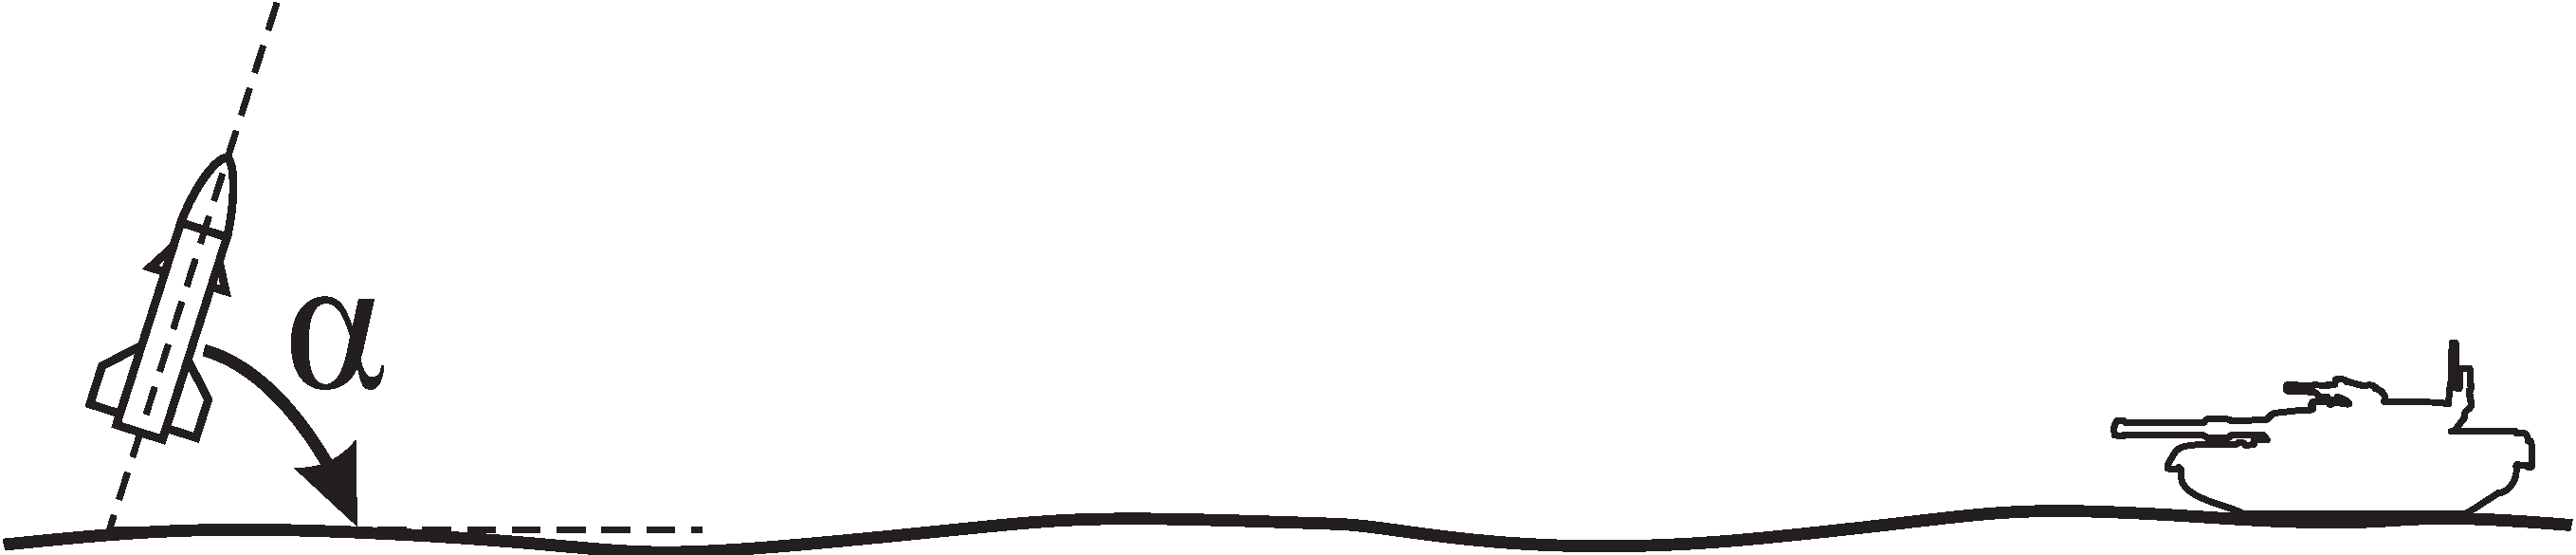
\includegraphics[width=0.475\textwidth]{rys05/alfa1} & 
  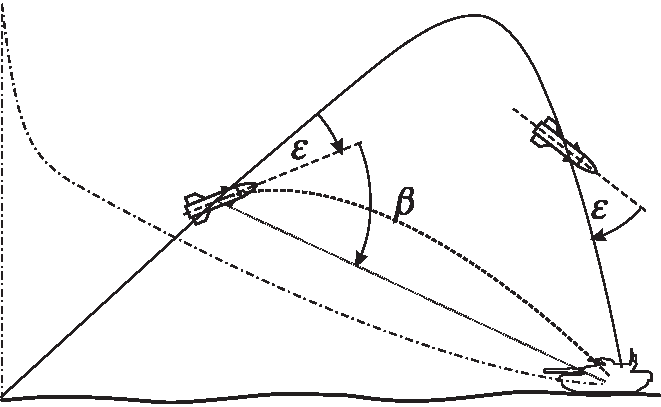
\includegraphics[width=0.475\textwidth]{rys05/beta1}
	% jeśli obraki są różnej wysokości, można je wyrównać do góry stosując vtop jak niżej
	% \vtop{\vskip-2ex\hbox{{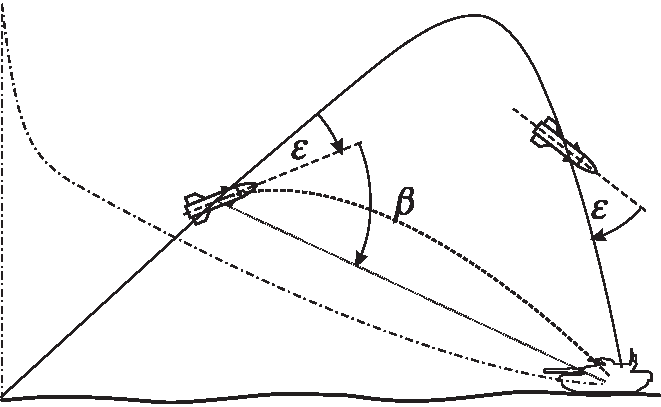
\includegraphics[width=0.475\textwidth]{rys05/beta1}}}} &
	% \vtop{\vskip-2ex\hbox{{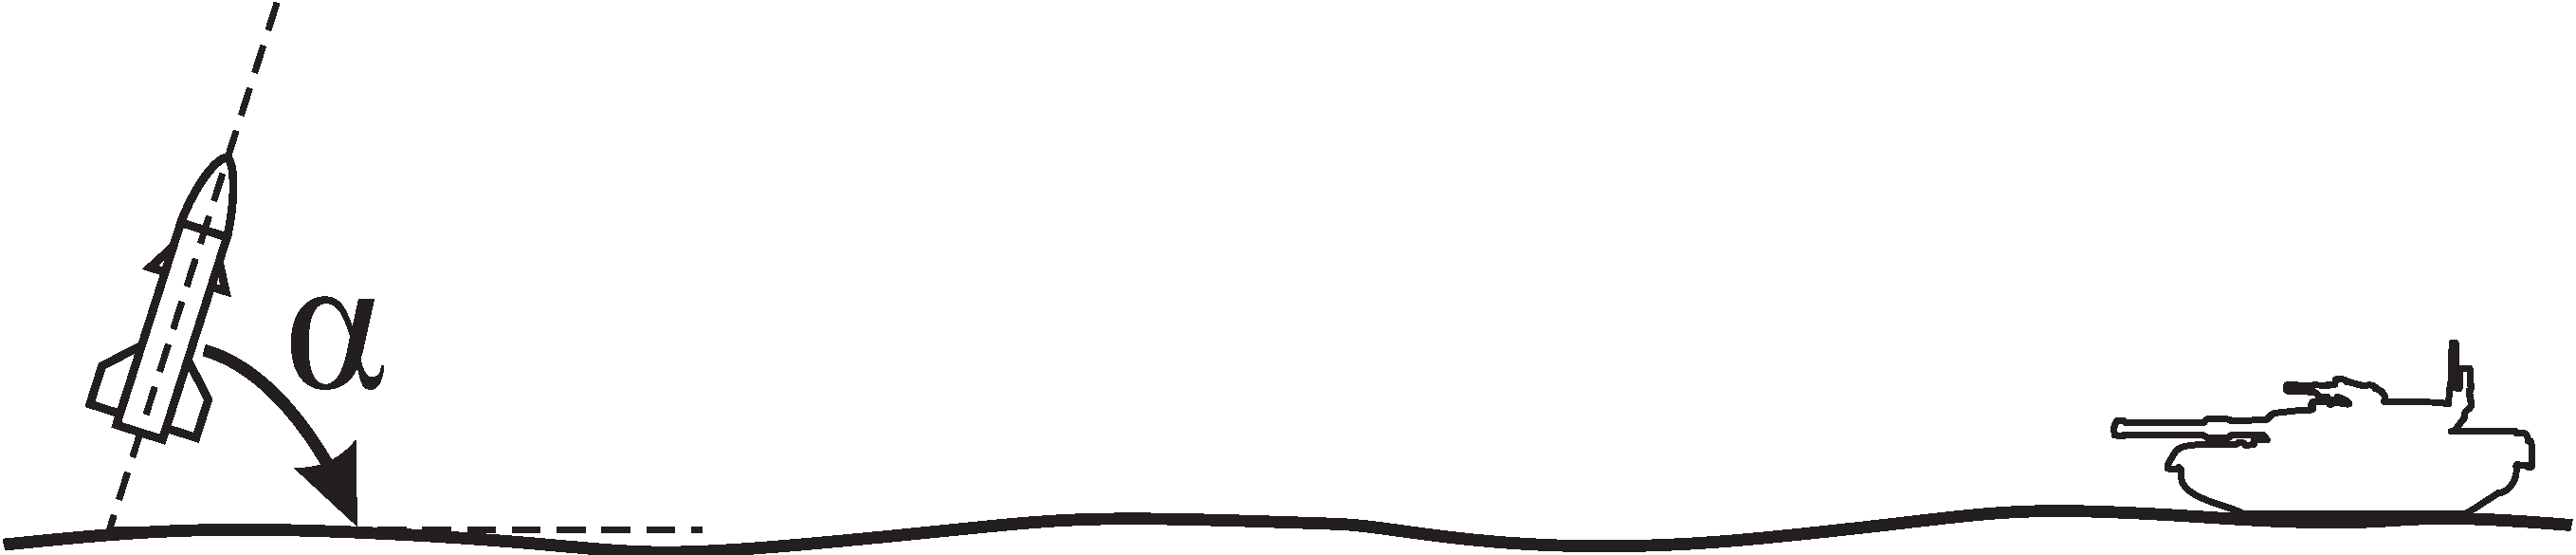
\includegraphics[width=0.475\textwidth]{rys05/alfa1}}}} 
  \end{tabular}
 a) trzy podejścia, b) podejście praktyczne}
 \label{fig:alfabeta}
\end{figure}
\end{lstlisting}

\begin{figure}[ht]
	\centering
		
\includegraphics[width=0.3\linewidth]{rys05/kanji-giri}
	\caption{Dwa znaki kanji -- giri}
	\label{fig:kanji-giri}
\end{figure}

\begin{figure}[htb]
  \centering
	\begin{tabular}{@{}ll@{}}
	a) & b) \\
  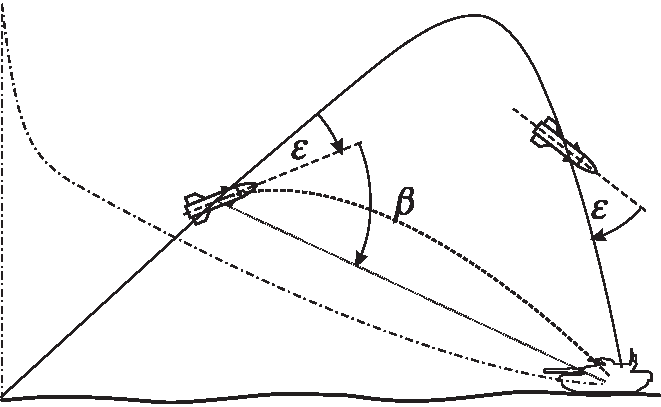
\includegraphics[width=0.475\textwidth]{rys05/beta1} & 
	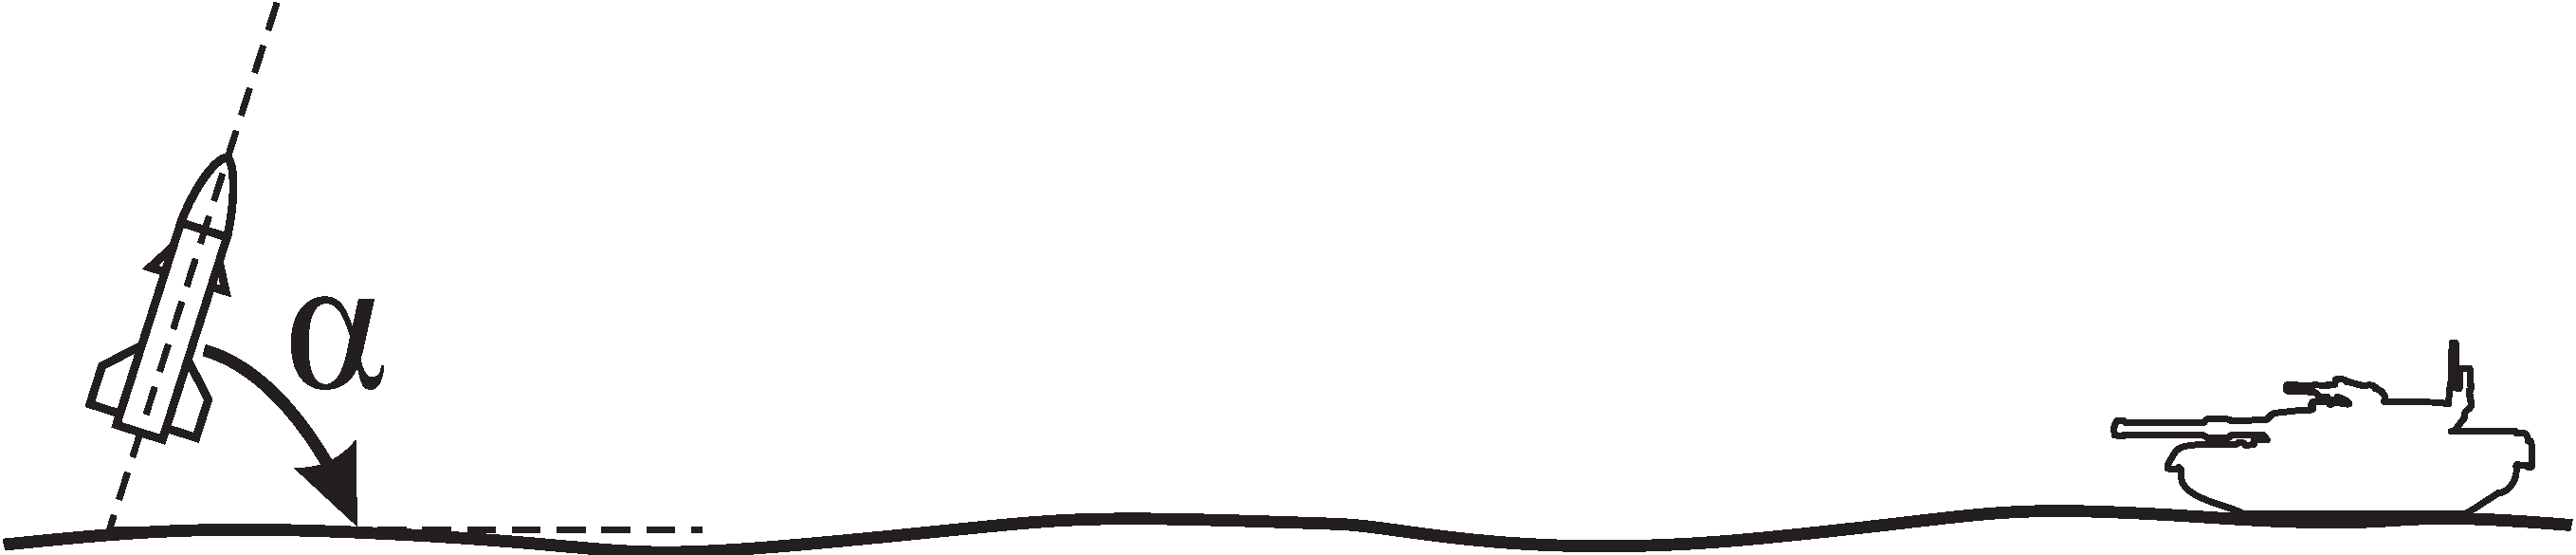
\includegraphics[width=0.475\textwidth]{rys05/alfa1}
	% jeśli obraki są różnej wysokości, można je wyrównać do góry stosując vtop jak niżej
	% \vtop{\vskip-2ex\hbox{{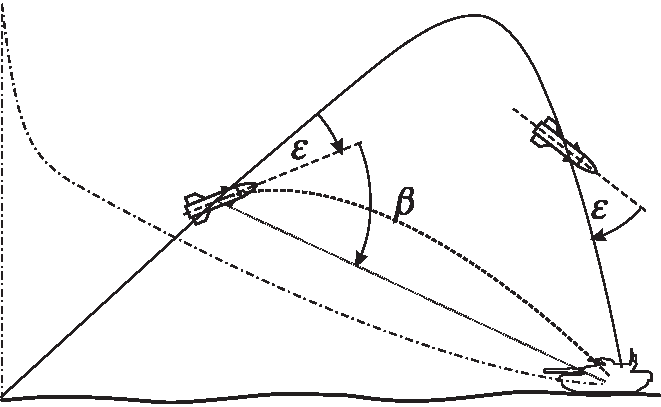
\includegraphics[width=0.475\textwidth]{rys05/beta1}}}} &
	% \vtop{\vskip-2ex\hbox{{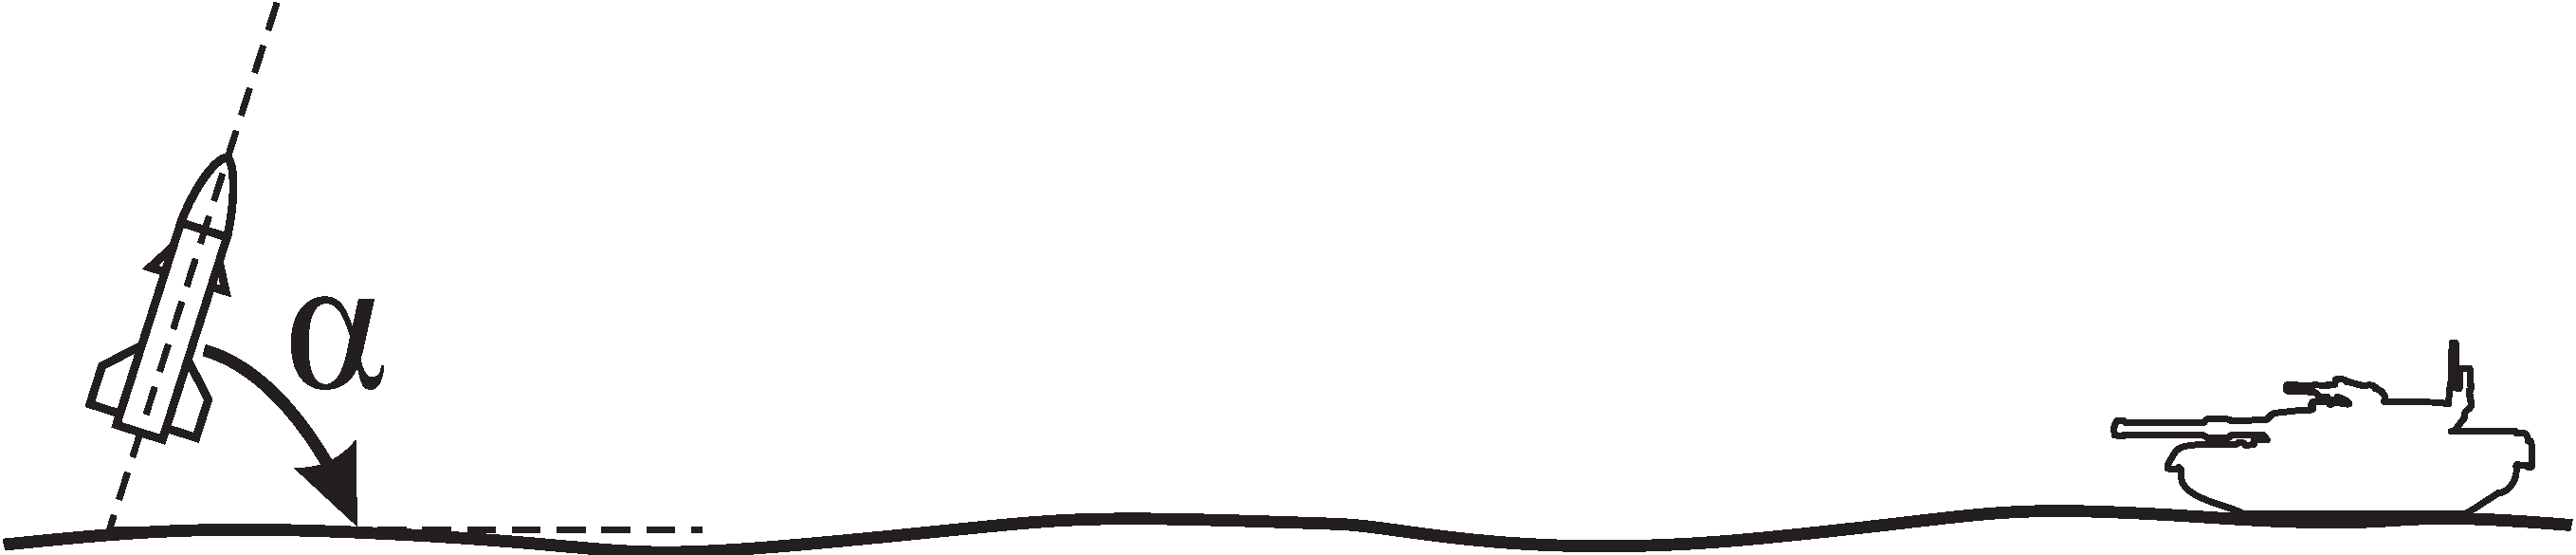
\includegraphics[width=0.475\textwidth]{rys05/alfa1}}}}  \caption{Wyznaczanie trajektorii lotu rakiety: 
	\end{tabular}
  \caption{Wyznaczanie trajektorii lotu rakiety: a) trzy podejścia, b) podejście praktyczne}
  \label{fig:alfabeta}
\end{figure}

Grafiki wektorowe powinny być dostarczone w plikach pdf. Rozmiar strony w~pliku pdf powinien być równy lub minimalnie większy od rozmiaru znajdującej się na nim grafiki (proszę spojrzeć na przykłady grafik wykorzystanych w niniejszym szablonie). Chodzi o to, aby na rysunku nie pojawiała się niepotrzebna biała przestrzeń (rozmiar płótna ma odpowiadać rozmiarowi grafiki bez żadnych marginesów, elementy grafiki powinny być ciasno ułożone). Grafiki rastrowe (głównie zrzuty z ekranu bądź zdjęcia) powinny być dostarczane w plikach o formacie \texttt{png} z~kompresją bezstratną. Zastosowanie kompresji stratnej, jak \texttt{jpg}, wprowadza niepotrzebne artefakty. Podobnie jak w przypadku grafik wektorowych, grafiki rastrowe nie powinny mieć białych marginesów.

Niezłym sposobem generowanie ładnej grafiki wektorowej, w szczególności diagramów, jest posłużenie się, kolejno, następującymi darmowymi narzędziami:
\begin{itemize}
\item w \texttt{diagrams.net} (dawniej \texttt{draw.io}): narysowanie diagramu i wyeksportowanie do pdf (bezpośrednio lub pośrednio, poprzez zapisanie pliku w formacie \texttt{svg}, a potem jego wyświetlenie w~przeglądarce internetowej i wydrukowanie do \texttt{pdf}),
\item w \texttt{inkscape}: zaimportowanie \texttt{pdf}, rozdzielenie grupy, wykasowanie niepotrzebnych elementów (tła), zaznaczenie wszystkiego, przycięcie strony do zaznaczonych (Ctr-Shift-R), zapisanie jako \texttt{pdf}. 
\end{itemize}

Na rysunku~\ref{fig:diagramy} pokazano przykład dobrze i źle (od strony technicznej) narysowanego diagramu. Celowo pokazano ramki, by było widać marginesy. Normalnie ramek tych nie należy stosować.
\begin{figure}[htb]
  \centering
	\begin{tabular}{@{}ll@{}}
	a) & b) \\
  \vtop{\vskip-2ex\hbox{\fbox{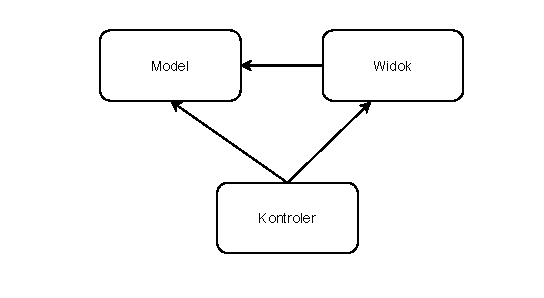
\includegraphics[width=0.4\linewidth]{rys05/diagram1}}}} & 
	\vtop{\vskip-2ex\hbox{\fbox{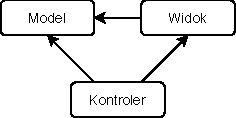
\includegraphics[width=0.4\linewidth]{rys05/diagram2}}}}
	% jeśli obraki są różnej wysokości, można je wyrównać do góry stosując vtop jak niżej
	% \vtop{\vskip-2ex\hbox{{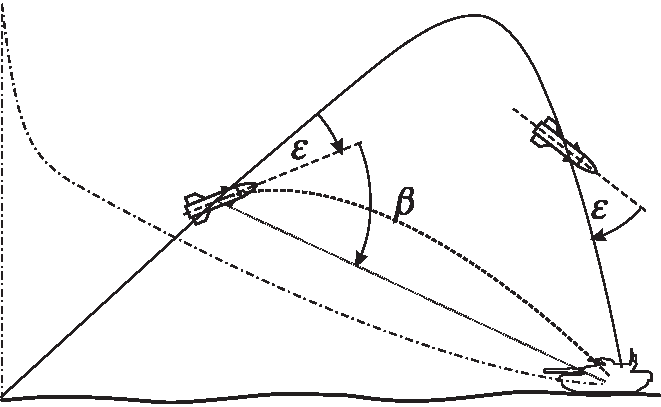
\includegraphics[width=0.475\textwidth]{rys05/beta1}}}} &
	% \vtop{\vskip-2ex\hbox{{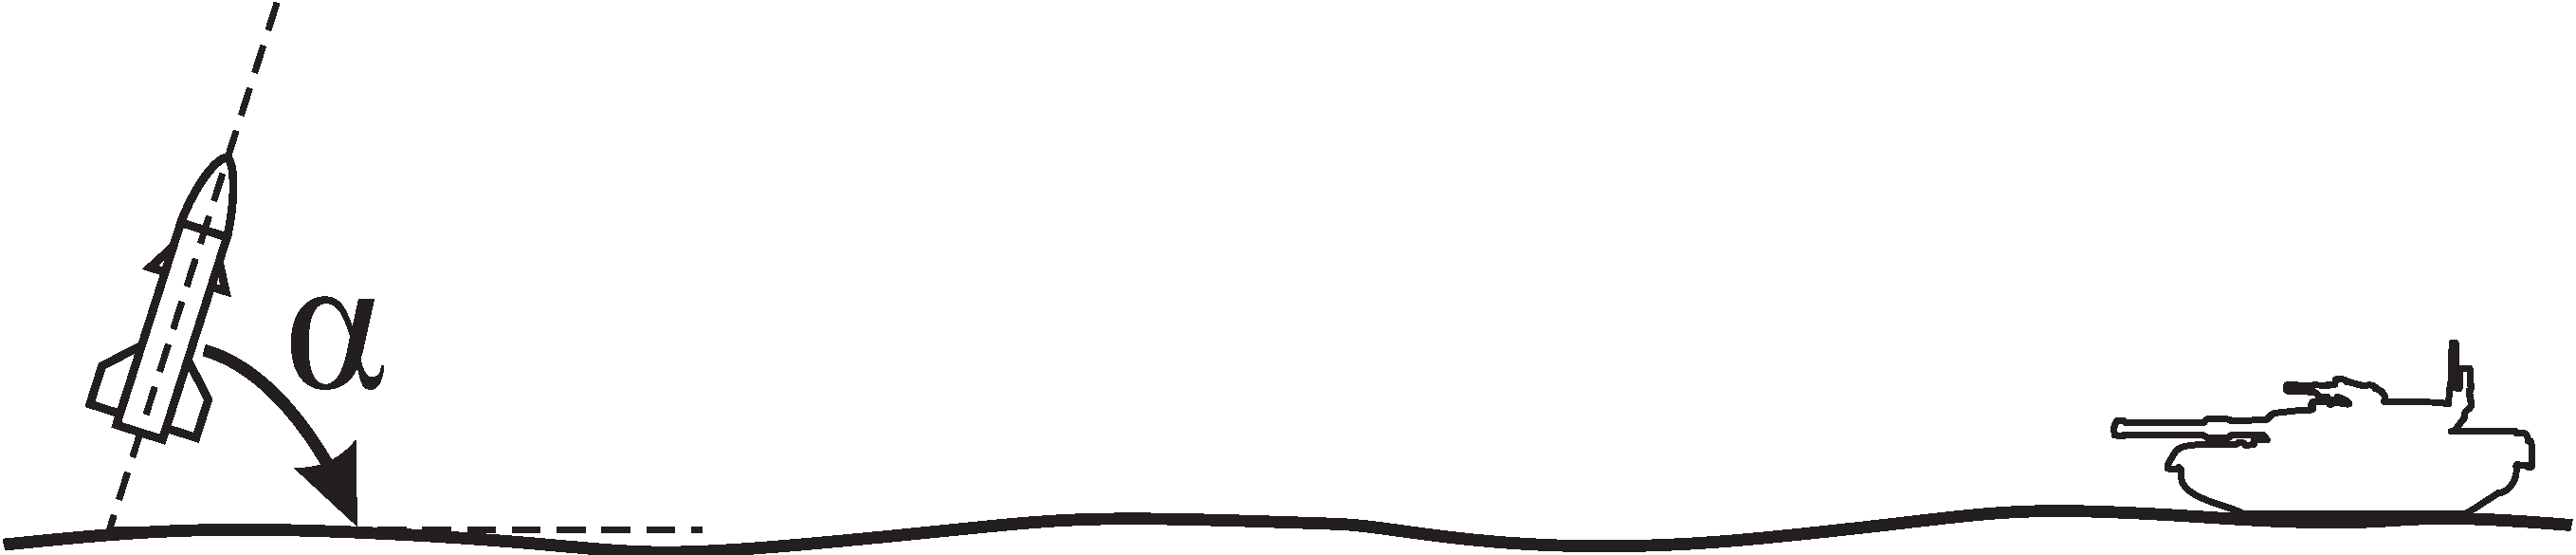
\includegraphics[width=0.475\textwidth]{rys05/alfa1}}}}  \caption{Wyznaczanie trajektorii lotu rakiety: 
	\end{tabular}
  \caption{Przykład diagramu: a) złego, b) w miarę dobrego}
  \label{fig:diagramy}
\end{figure}

Elementy na rysunkach nie powinny być wypełnione 100\% czernią ponieważ na wydrukach tworzą się plamy przebijające się przez kartkę. Zamiast tego wypełnienie elementów powinno być ustawione na ok.\ 90\% czerni.

Czcionka na rysunkach nie może być większa od czcionki wiodącej tekstu (jedyny wyjątek to np.\ jakieś nagłówki).
Należy stosować czcionkę kroju Arial, Helvetica bądź tego samego kroju co czcionka dokumentu (\texttt{texgyre-termes}). 

Jeśli na jednym rysunku pojawić się ma kilka grafik, to zamiast stosować \texttt{subfigure} lub inne otoczenia należy: dostarczyć tabelę z wstawionymi do niej rysunkami, opcjonalnie adnotować jej części (np.~a) i b)), odnieść się do tych części w podpisie (posługując się adnotacjami, jak to zrobiono na rysunkach~\ref{fig:alfabeta} i \ref{fig:diagramy}, lub opisem słownym, np.~,,z lewej strony pokazano ...'', ,,po prawej zamieszczono ...'').

Jeśli na rysunku zamieszczono w tabeli kilka grafik, to ich pozycjonowaniem (wyjustowaniem od góry) można manipulować za pomocą komendy:
\verb+\vtop{\vskip-2ex\hbox{\includegraphics[width=0.475\textwidth]{nazwa}}}+

Na rysunkach nie wolno nadużywać kolorów oraz ozdobników (wiele narzędzi do tworzenia diagramów dostarcza grafikę z cieniowaniem, gradacją kolorów itp.\  co niekoniecznie przekłada się na czytelność rysunku).
Jeśli rysunki są kolorowe, to kolory te powinny być rozróżnialne po konwersji do poziomów szarości (chodzi o to, aby na wydrukach wykonanych na drukarkach monochromatycznych można było dostrzec różnice).

Podczas robienia zrzutów z ekranu należy zadbać o to, by taki zrzut był czytelny po wydrukowaniu. Czyli aby pojawiające się literki były wystarczająco duże, a przestrzenie bez treści -- relatywnie małe. Przystępując do robienia zrzutu trzeba odpowiednio wyskalować elementy na ekranie. Na przykład robiąc zrzut z przeglądarki FF najpierw należy wcisnąć CTR--0 (domyślne skalowanie), potem CTR--{}- (zmniejszenie skali o stopień). Potem dobrze jest zawęzić okno przeglądarki tak, by interesująca treść wypełniła je w całości. Jeśli na obserwowanej stronie jest zbyt dużo pustych obszarów, to należy je jakoś zawęzić (sterując wielkością okna przeglądarki lub aktywnymi elementami interfejsu użytkownika). Zrzut bowiem wcale nie musi być odzwierciedleniem 1:1 domyślnego układu obserwowanych elementów. Ważne jest, by na zrzucie pokazać interesujący, opisywany fragment i żeby ten fragment był czytelny. Nie trzeba też zawsze robić zrzutów w układzie 16:9 (lub innym panoramicznym). Czasem lepiej jest zrobić zrzuty okien niemal kwadratowych, bo lepiej się układają w wynikowym dokumencie. Poza tym można je przeskalować (powiększyć) by zajmowały całą szerokość strony, a wtedy czcionka na wydrukach będzie większa. Takie skalowanie dla zrzutów panoramicznych zwykle się nie udaje. Na rysunku~\ref{fig:zrzuty} pokazano przykłady dobrze i źle zrobionych zrzutów (w celu oszczędzenia miejsca zrzuty umieszczono obok siebie).
	
\begin{figure}[htb]
  \centering
	\begin{tabular}{@{}ll@{}}
	a) & b) \\
  \vtop{\vskip-2ex\hbox{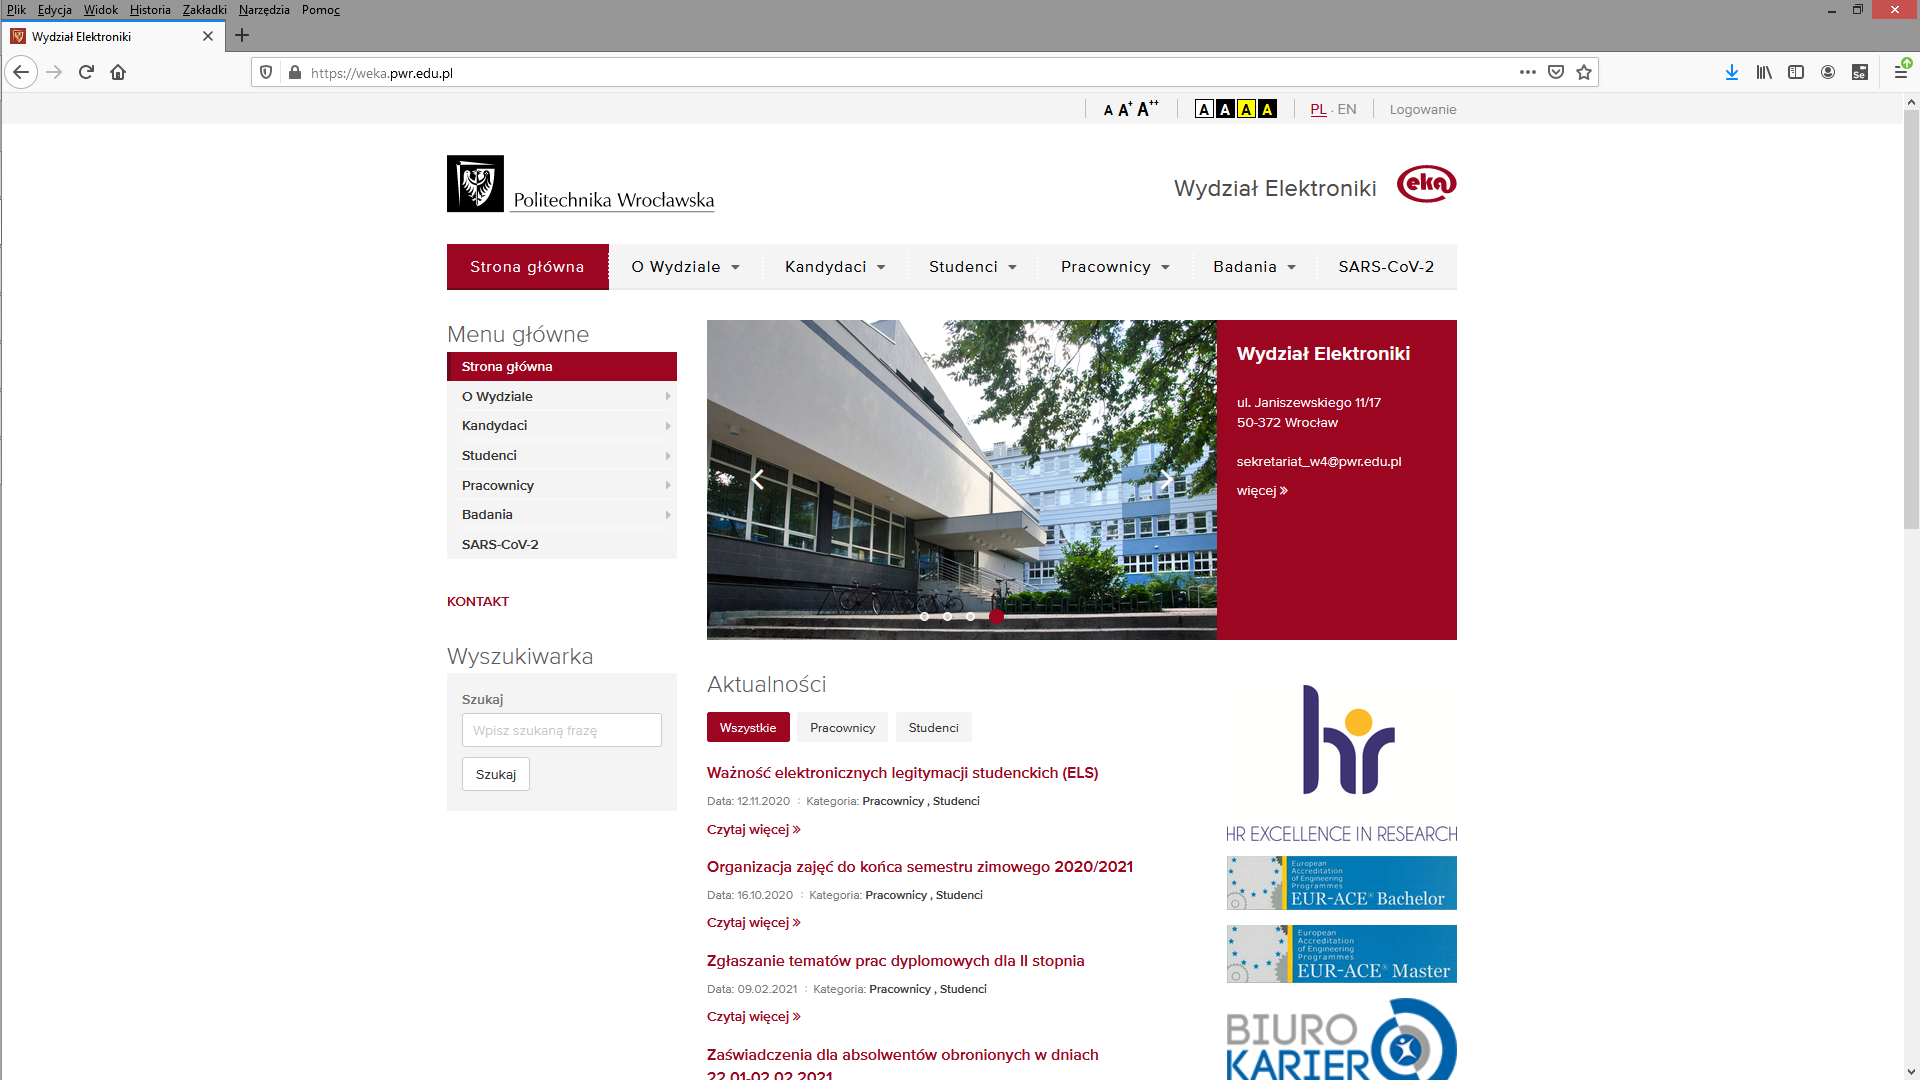
\includegraphics[width=0.475\textwidth]{rys05/zrzut1}}} & 
	\vtop{\vskip-2ex\hbox{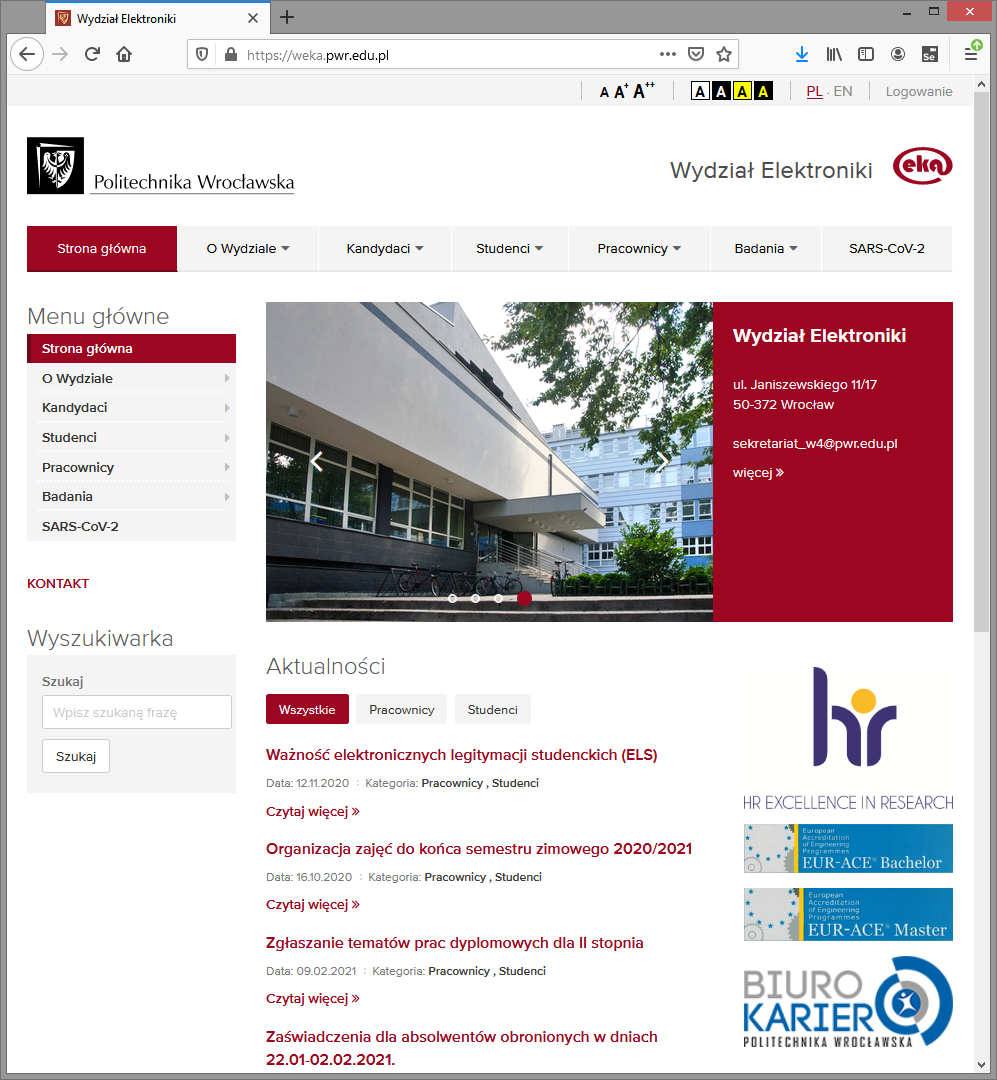
\includegraphics[width=0.475\textwidth]{rys05/zrzut2}}}
	% jeśli obraki są różnej wysokości, można je wyrównać do góry stosując vtop jak niżej
	% \vtop{\vskip-2ex\hbox{{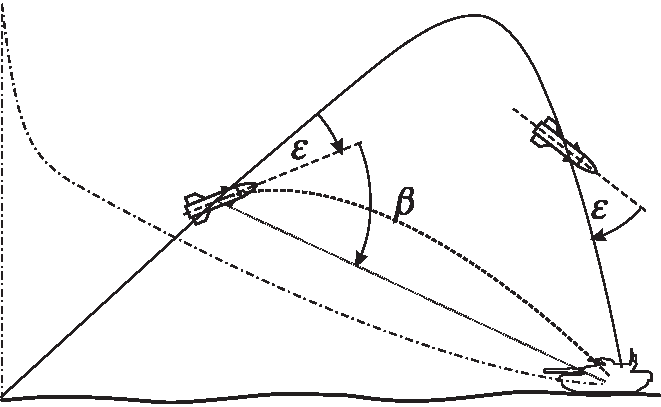
\includegraphics[width=0.475\textwidth]{rys05/beta1}}}} &
	% \vtop{\vskip-2ex\hbox{{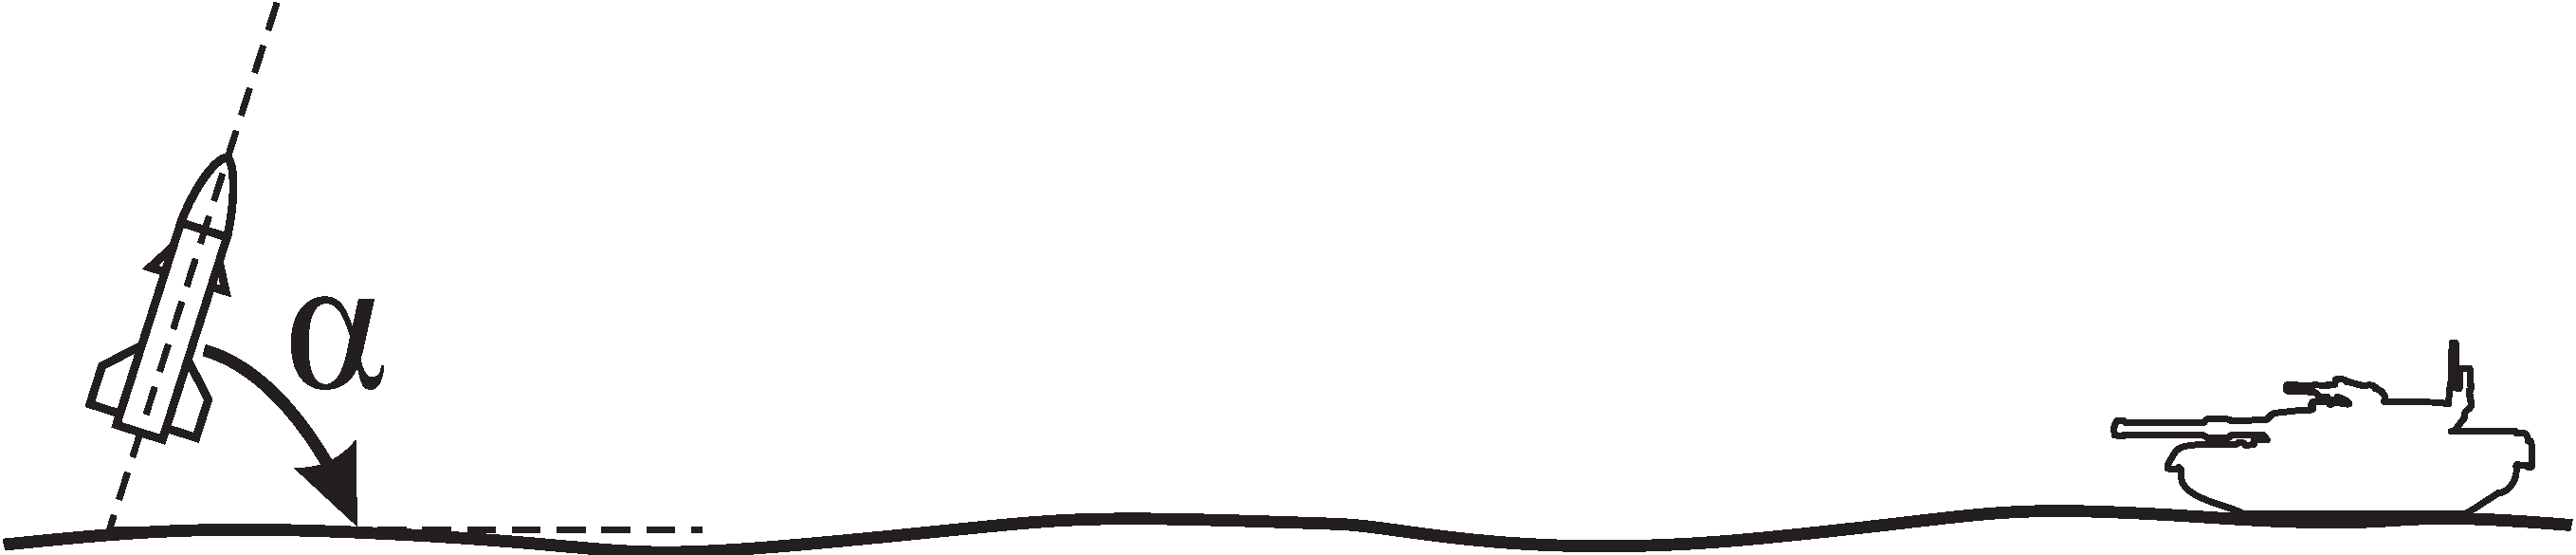
\includegraphics[width=0.475\textwidth]{rys05/alfa1}}}}  \caption{Wyznaczanie trajektorii lotu rakiety: 
	\end{tabular}
  \caption{Przykłady zrzutów z ekranu: a) zły (nieczytelny, zrobiony przy zbyt szerokim oknie, z niepotrzebnymi marginesami, niepotrzebnym paskiem menu), b) w miarę dobry (w miarę czytelny, zrobiony przy zawężonym oknie, byłoby wskazane jeszcze usunięcie z niego beleczki z faviconem (jeśli nic nie wnosi) oraz przycięcie od dołu (jeśli treści tam pokazywane nie są istotne))}
  \label{fig:zrzuty}
\end{figure}

	
Czasem problemem jest tworzenie zrzutów z ekranu, gdy występują na nim dane wrażliwe. Istnieją dwa sposoby na radzenie sobie z tym problemem.
Pierwszy polega na zastąpieniu w~systemie danych danych rzeczywistych danymi testowymi -- wygenerowanymi tylko do celów prezentacji.
Zrzut robi się wtedy na bazie danych testowych.
Drugi polega na wykonaniu zrzutu z~ekranu, na którym pokazano dane rzeczywiste, i następnie zamianie tych danych już w pliku graficznym
za pomocą odpowiedniego edytora (np.~\texttt{gimp}). Czyli oryginalny zrzut z ekranu należy otworzyć w edytorze, a potem
nadpisać oryginalny tekst własnym tekstem. Konieczne jest wtedy dobranie odpowiednich czcionek aby nie było widać
wprowadzonych zmian. 
\begin{quotation}
Uwaga: takie manipulowanie zrzutami jest usprawiedliwione jedynie w przypadku konieczności ochrony danych wrażliwych czy też lepszego pokazania wybranych elementów. Nie może to prowadzić generowania fałszywych rezultatów!!!
\end{quotation}

\section{Wstawianie kodu źródłowego}
Kod źródłowy można wstawiać jako blok tekstu pisany czcionką maszynową. Używa się do tego otoczenie \verb?\lstlisting?. W atrybutach otoczenia można zdefiniować tekst podpisu wstawianego wraz z numerem nad blokiem, etykietę do tworzenia odwołań, sposób formatowania i~inne ustawienia. Zaleca się stosowanie w tym otoczeniu następujących parametrów:
\begin{lstlisting}[basicstyle=\footnotesize\ttfamily]
\begin{lstlisting}[label=list:req1,caption=Initial HTTP Request,
                   basicstyle=\footnotesize\ttfamily]
\end{lstlisting}
Szczególnie przydatne podczas wstawiania większej ilości kodu źródłowego jest zastosowanie parametru \verb+basicstyle=\footnotesize\ttfamily+. Dzięki niemu zmniejsza się czcionka, a~przez to na stronie można zmieścić dłuższe linijki kodu. Użycie tak zdefiniowanego parametru nie jest jednak sztywnym zaleceniem. Wielkość czcionki można dobierać do potrzeb. 
{\belowcaptionskip=-10pt
\begin{lstlisting}[label=list:req1,caption=Initial HTTP Request,
                   basicstyle=\footnotesize\ttfamily]
GET /script/Articles/Latest.aspx HTTP/1.1
Host: www.codeproject.com
Connection: keep-alive
Cache-Control: max-age=0
Accept: text/html,application/xhtml+xml,application/xml
User-Agent: Mozilla/5.0 ...
Accept-Encoding: gzip,deflate,sdch
Accept-Language: en-US...
Accept-Charset: windows-1251,utf-8...
\end{lstlisting}
}
Można też sformatować kod bez stosowania numerowanego podpisu (wtedy nie zamieszcza się \texttt{caption} na liście atrybutów).
\begin{lstlisting}[basicstyle=\footnotesize\ttfamily]
GET /script/Articles/Latest.aspx HTTP/1.1
Host: www.codeproject.com
Connection: keep-alive
Cache-Control: max-age=0
Accept: text/html,application/xhtml+xml,application/xml
User-Agent: Mozilla/5.0 ...
Accept-Encoding: gzip,deflate,sdch
Accept-Language: en-US...
Accept-Charset: windows-1251,utf-8...
\end{lstlisting}

Ponadto istnieje kilka sposobów wstawiania kodu źródłowego w bieżącej linijce tekstu:
\begin{itemize} 
\item korzystając z polecenia \verb?\texttt? ustawiającego czcionkę maszynową, jak w przykładzie \texttt{tutaj} (efekt zastosowania komendy \verb?\texttt{tutaj}?). Problemem jednak mogą okazać się znaki podkreślenia i inne znaki kontrolne.
\item korzystają z otoczenia \verb?\verb? zapewniającego wypisanie kodu czcionką maszynową jak w~przykładzie \verb|tutaj| (efekt zastosowania komendy \verb?\verb|tutaj|?). Problemem jest to, że polecenie \verb?\verb? nie potrafi łamać dłuższego tekstu.
\item korzystając z polecenia \verb?\lstin? umożliwiającego wypisanie kodu czcionką ustawianą w~opcjach jak w przykładzie
\lstset{basicstyle=\ttfamily}\lstinline{tutaj} (efekt komendy \verb+\lstset{basicstyle=\ttfamily}\lstinline{tutaj}+) lub \lstinline[basicstyle=\ttfamily]=tutaj= (efekt komendy \verb+\lstinline[basicstyle=\ttfamily]=tutaj=+).
\end{itemize}

Poniżej zamieszczono przykłady kodów źródłowych z podświetleniem składni.

\begin{lstlisting}[language=Java,style=JavaStyle,caption=Opis 1, label=lst:pierwszy]
package pl.mrbarozoit.backend;

import org.springframework.boot.SpringApplication;
import org.springframework.boot.autoconfigure.SpringBootApplication;

@SpringBootApplication
public class BackendApplication {

    public static void main(String[] args) {
        SpringApplication.run(BackendApplication.class, args);
    }

}
\end{lstlisting}

Jeśli w kodzie źródłowym jest jakiś nieistotny fragment względem omawianego problemu, to można go wykropkować (patrz listing~\ref{lst:drugi}).

{\belowcaptionskip=-9pt % To polecenie zmniejszy odległość podpisu od pokazywanego kodu (jego stosowanie jest zalecane)
\begin{lstlisting}[language=JavaScript,style=JavaScriptStyle,caption=Opis 2, label=lst:drugi]
// Karma configuration file, see link for more information
// https://karma-runner.github.io/1.0/config/configuration-file.html

module.exports = function (config) {
  config.set({
    basePath: '',
    frameworks: ['jasmine', '@angular-devkit/build-angular'],
    plugins: [
      require('karma-jasmine'),
      require('karma-chrome-launcher'),
      require('karma-jasmine-html-reporter'),
      require('karma-coverage-istanbul-reporter'),
      require('@angular-devkit/build-angular/plugins/karma')
    ],
    ... // opuszczony kod
    autoWatch: true,
    browsers: ['Chrome'],
    singleRun: false,
    restartOnFileChange: true
  });
};
\end{lstlisting}
}

Jeśli kod jest wąski, to można sformatować go w dwóch kolumnach jak na listingu~\ref{lst:kontrakt-board-move-in}.

% Trzeba zacząć po linijce przerwy
\begingroup 
\listingcaption{Kontrakt na model wejściowy endpointu \texttt{/api/v1/chess/board/move}}
\setlength\multicolsep{0pt plus 2pt}%
\begin{lstlisting}[style=json-style, multicols=2, label=lst:kontrakt-board-move-in]
{
   "lastPosition": {
      "fenDescription": "string"
   },
   "image": {
      ...
   },
   "positions": {
      "chessboardCorners": [
         ...
      ],
      "tilesCornerPoints": [
         ...
      ]
   },
   "referenceColors": {
      ...
   },
}
\end{lstlisting}
\vspace{6pt plus 2pt}
\endgroup

\section{Wykaz literatury oraz cytowania}
\label{sec:literatura}
Cytowania powinny być zamieszczane w tekście z użyciem komendy \verb+\cite{}+. Jej argumentem powinien być klucz cytowanej pozycji (lub lista kluczy  rozdzielonych przecinkiem bez spacji, jeśli takich pozycji w danym miejscu cytuje się więcej) jaki jest używany w bazie danych bibliograficznych (plik \texttt{dokumentacja.bib}). Po kompilacji \texttt{bibtex} i \texttt{pdflatex} w tekście pojawia się właściwy odsyłacz do pozycji w wykazie literatury (ujęty w kwadratowe nawiasy -- zgodnie z~tym, co definiuje styl \texttt{plabbrv.bst}), zaś w samym wykazie (rozdział Literatura) -- zacytowana pozycja. Przykładem cytowania jest: ,,dobrze to opisano w pracach~\cite{JS07,SQL2}'' (gdzie zastosowano komendę \verb?\cite{JS07,SQL2}?).

Co do zawartości rekordów bibliograficznych - style bibtexowe potrafią ,,skracać'' imiona (czyli wstawiać, jeśli taka wola, inicjały zamiast pełnych imion). Niemniej dobrze jest od razu przyjąć jakąś konwencję. Proponuje się, aby w rekordach od razu wstawiane były inicjały zamiast pełnych imion.

Niekiedy tytuły prac zawierają wyrazy z dużymi i małymi literami. Takie tytuły należy brać w podwójne nawiasy klamrowe, aby \texttt{bibtex} nie zamienił ich na postać, w której poza pierwszą literą pozostałe są małe.

Jeśli jakiś cytowany zasób pochodzi z Internetu, to jego rekord w pliku \texttt{bib} powinien wyglądać jak niżej.
\begin{lstlisting}[basicstyle=\footnotesize\ttfamily]
@INPROCEEDINGS{SQL2, 
  title={{A MySQL-based data archiver: preliminary results}}, 
  author={Bickley, M. and Slominski, Ch.},
  booktitle = {{Proceedings of ICALEPCS07}},
	month = oct,
	day = {15--19},
	year={2007}, 
  note={\url{http://www.osti.gov/scitech/servlets/purl/922267} 
	[dostęp dnia 20 czerwca 2015]}
}
\end{lstlisting}
A to inny przykład rekordu danych bibliograficznych:
\begin{lstlisting}[basicstyle=\footnotesize\ttfamily]
@TechReport{JS07,
	author = {Jędrzejczyk, J. and Śródka, B.},
	title  ={Segmentacja obrazów metodą drzew decyzyjnych},
	year = {2007},
	institution = {Politechnika Wrocławska, Wydział Elektroniki}
}
\end{lstlisting}

\section{Indeks rzeczowy}
\label{sec:indeks}
Generowanie indeksu \index{generowanie!-- indeksu} po trosze wygląda jak generowanie wykazu literatury \index{generowanie!-- wykazu literatury}-- wymaga kilku kroków. Podczas pierwszej kompilacji \texttt{pdflatex} generowany jest plik z rozszerzeniem \texttt{*.idx} (zawierający ,,surowy indeks''). Następnie, bazując na tym pliku, generowany jest plik z rozszerzeniem \texttt{*.ind} zawierający sformatowane dane. Ten krok wymaga uruchomienia odpowiedniego narzędzia oraz zastosowania plik z definicją stylu \texttt{Dyplom.ist}. W kroku ostatnim dokonuje się kolejnej kompilacji \texttt{pdflatex} (dzięki niej w wynikowym dokumencie pojawi się Indeks rzeczowy). Domyślnie Indeks rzeczowy zostanie sformatowany w~układzie dwukolumnowym.

Oczywiście aby to wszystko zadziałało w kodzie szablonu należy umieścić odpowiednie komendy definiujące elementy indeksu rzeczowego (\verb?\index?) oraz wstawiające sformatowany Indeks rzeczowy do dokumentu wynikowego (\verb?\printindex?). Więcej informacji o tworzeniu indeksu rzeczowego można znaleźć na stronie \url{https://en.wikibooks.org/wiki/LaTeX/Indexing}. Poniżej przedstawiono przykłady komend użytych w szablonie do zdefiniowania elementów indeksu rzeczowego:
\begin{itemize}
\item \verb?\index{linia komend}? -- pozycji główna.
\item \verb?\index{generowanie!-- indeksu}? -- podpozycja.
\end{itemize}

Generowanie pliku \texttt{*.ind} można inicjować na kilka sposobów:
\begin{itemize}
\item poprzez wydanie odpowiedniego polecenia bezpośrednio w linii komend \index{linia komend}
\begin{lstlisting}[basicstyle=\footnotesize\ttfamily]
makeindex Dyplom.idx -t Dyplom.ilg -o Dyplom.ind -s Dyplom.ist
\end{lstlisting}
\item poprzez odpalenie odpowiedniego narzędzia środowiska. Na przykład w \texttt{TeXnicCenter} definiuje się tzw. \texttt{output profiles}: 
\begin{lstlisting}[basicstyle=\footnotesize\ttfamily]
makeindex "%tm.idx" -t "%tm.ilg" -o "%tm.ind" -s "%tm.ist"
\end{lstlisting}
a samo generowanie pliku \texttt{*.ind} zapewni wybranie pozycji menu \texttt{Build/Makeindex}.
\item korzystając z odpowiednio sparametryzowanych pakietów i komend wewnątrz kompilowanego dokumentu (czyli od razu przy okazji jego kompilacji).
\begin{lstlisting}[basicstyle=\footnotesize\ttfamily]
\DisemulatePackage{imakeidx}
\usepackage[noautomatic]{imakeidx} 
% jeśli chcemy, by indeks by generowany automatycznie programem makeindex:
%\usepackage[makeindex]{imakeidx} 
% a tak ponoć można przekazać opcje do programu generującego indeks:
%\makeindex[options=-s podrecznik -L polish -M lang/polish/utf8] 
%\makeindex[options=-s podrecznik]
\makeindex
\end{lstlisting}

Niestety, \texttt{makeindex} jest narzędziem, które umieszcza część pozycji w grupie \texttt{Symbols}, a~nie w grupach związanych z literkami alfabetu. W związku z czym indeksowany element zaczynający się od polskiej literki trafia do grupy \texttt{Symbols}, jak np.~\verb?\index{Światło}?\index{Światło}. Jeśli chce się zamieszczać w indeksie symbole matematyczne, to dobrze jest to robić jak w następującym przykładzie: \verb?\index{$asterisk@$\ast$}? \index{$asterisk@$\ast$} czy też \verb?\index{c@$\mathcal{C}$}?\index{c@$\mathcal{C}$}, tj.~dostarczając przy okazji klucz do sortowania.
Lepiej w tym względzie radzą sobie inne narzędzia, jak \texttt{texindy} lub \texttt{xindy} dostępne pod linuxem. Korzystając z nich uzyskuje się grupy polskich literek w indeksie rzeczowym (hasła zaczynające się od polskich literek już nie trafiają do grupy Symbols). Przykład polecenia wydanego z linii komend, w którym wykorzystano \texttt{texindy} zamieszczono poniżej (zakładamy kodowanie plików w UTF8, można dla niniejszego szablonu zmienić na cp1250):
\begin{lstlisting}[basicstyle=\footnotesize\ttfamily]
texindy -L polish -M lang/polish/utf8 Dyplom.idx
\end{lstlisting}

To polecenie wygeneruje \texttt{Dyplom.ind} o zawartości:
\begin{lstlisting}[basicstyle=\footnotesize\ttfamily]
\begin{theindex}
  \providecommand*\lettergroupDefault[1]{}
  \providecommand*\lettergroup[1]{%
      \par\textbf{#1}\par
      \nopagebreak
  }

  \lettergroup{G}
  \item generowanie
    \subitem -- indeksu, 27
    \subitem -- wykazu literatury, 27

  \indexspace

  \lettergroup{L}
  \item linia komend, 27

  \indexspace

  \lettergroup{Ś}
  \item \'Swiat\IeC {\l }o, 28

\end{theindex}
\end{lstlisting}


\end{itemize}


Aby mieć większą kontrolę automatyczne generowanie indeksu zostało w niniejszym szablonie wyłączone (indeks trzeba wygenerować samemu, wydając polecenie \texttt{makeindex} lub zalecane \texttt{texindy}).

\section{Inne uwagi}
Dobrym sposobem na kontrolę błędów występujących podczas kompilacji jest wstawianie linijki \verb?\end{document}? w wybranym miejscu dokumentu. Jest to szczególnie przydatne w przypadkach, gdy błędy te są trudne do zidentyfikowania (gdy wygenerowane przez kompilator numery linii z błędami nie są tymi, w których błędy występują). Wystarczy wtedy przestawić wspomnianą linijkę do kolejnych miejsc, aż znajduję to miejsce, gdzie występuje problem.

Aby osiągnąć apostrofy maszynowe (złożone z samych kresek) należy użyć polecenia \verb?"{}jak tutaj{}"? (podwójny apostrof stojący bezpośrednio przed niektórymi literkami zamienia je na literki z akcentami, aby temu zapobiec dostawiono nawiasy klamrowe). W efekcie otrzymamy "{}jak tutaj{}". Jeśli natomiast apostrofy mają być drukarskie (złożone z kropek i kresek), to należy użyć polecenia \verb?,,jak tutaj''? (dwa pojedyncze przecinki i dwa pojedyncze apostrofy). W efekcie otrzymamy ,,jak tutaj''. Można też użyć znaków apostrofów odpowiednio zakodowanych „jak tutaj”, tylko że czasem trudno pisze się takie apostrofy w środowiskach kompilacji projektów latexowych.


Oto sposoby ustawienia odstępów między liniami:
\begin{itemize}
\item używając komendy \verb+\linespread{...}+ (akceptowalne), przy czym atrybutem tej metody jest współczynnik zależny od wielkości
czcionki.  Dla czcionki wiodącej 12pt odstęp półtora linii osiągnie się komendą \verb+\linespread{1.241}+. Dla innych czcionek wiodących wartości tego parametru są jak w poniższym zestawieniu.
\begin{lstlisting}[basicstyle=\footnotesize\ttfamily]
10pt 1.25 dla \onehalfspacing 
     1.667 for \doublespacing, 
		 ponieważ ,,basic ratio'' = 1.2 
		(\normalfont posiada \baselineskip rozmiaru 12pt)
11pt 1.213 dla \onehalfspacing oraz 1.618 dla \doublespacing, 
     ponieważ ,,basic ratio'' = 1.236 
		(\normalfont posiada \baselineskip rozmiaru 13.6pt)
12pt 1.241 dla \onehalfspacing oraz 1.655 dla \doublespacing, 
     ponieważsince ''basic ratio'' is 1.208 
		(\normalfont has a \baselineskip of 14.5pt)
\end{lstlisting}
Kłopot w tym, że raz ustawiony odstęp będzie obowiązywał do wszystkich czcionek (brak jest mechanizmu zmiany współczynnika w zależności od wielkości czcionki akapitu).

\item używając pakietu \texttt{setspace} (niezalecane). Ponieważ klasa \texttt{memoir} emuluje pakiet \texttt{setspace}, w preambule dokumentu należałoby umieścić:
\begin{lstlisting}[basicstyle=\footnotesize\ttfamily]
\DisemulatePackage{setspace}
\usepackage{setspace}
\end{lstlisting}
a potem można już sterować odstęp komendami:
\begin{lstlisting}[basicstyle=\footnotesize\ttfamily]
\singlespacing
\onehalfspacing
\doubelspacing
\end{lstlisting}
Ten sposób pozwala na korzystanie z mechanizmu automatycznej zmiany odległości linii w~zależności od wielkości czcionki danego akapitu.
\item korzystając bezpośrednio z komend dostarczonych w klasie \texttt{memoir} (zalecane):
\begin{lstlisting}[basicstyle=\footnotesize\ttfamily]
\SingleSpacing
\OnehalfSpacing
\DoubleSpacing
\end{lstlisting}
Ten sposób również pozwala na korzystanie z mechanizmu automatycznej zmiany odległości linii w zależności od wielkości czcionki danego akapitu.
\end{itemize}

Na koniec jeszcze uwaga o rozmiarze pliku wynikowego. Otóż \texttt{pdflatex} generuje pliki \texttt{pdf}, które zazwyczaj mogłyby być nieco lepiej
skompresowane. Do lepszego skompresowania tych plików można użyć programu \texttt{ghostscript}. Wystarczy w tym celu wydać komendę (pod windowsami):
\begin{lstlisting}[basicstyle=\footnotesize\ttfamily]
gswin64 -sDEVICE=pdfwrite -dCompatibilityLevel=1.4 -dNOPAUSE -dQUIET \
-dSAFER -dBATCH -sOutputFile=Dyplom-compressed.pdf Dyplom.pdf
\end{lstlisting}
W poleceniu tym można również wstawić opcję \texttt{-dPDFSETTINGS=/prepress} (zapewniającą uzyskanie wysokiej jakości, zachowanie kolorów, uzyskanie obrazków w rozdzielczości 300 dpi). Ze względów licencyjnych ghostscript używa domyślnie algorytmów z kompresją stratną. Przy kompresji może więc dojść do utraty jakości bitmap.

\chapter{Podsumowanie}
\label{chap:podsumowanie}
Podsumowanie jest miejscem, w którym należy zamieścić syntetyczny opis tego, o czym jest dokument. W szczególności w pracach dyplomowych w podsumowaniu powinno znaleźć się jawnie podane stwierdzenie dotyczące stopnia realizacji celu. Czyli powinny pojawić się w niej akapity ze zdaniami typu: ,,Podczas realizacji pracy udało się zrealizować wszystkie postawione cele''. Ponadto powinna pojawić się dyskusja na temat napotkanych przeszkód i sposobów ich pokonania, perspektyw dalszego rozwoju, możliwych zastosowań wyników pracy itp. 

\section{Sekcja poziomu 1}% 
Lorem ipsum dolor sit amet eleifend et, congue arcu. Morbi tellus sit amet, massa. Vivamus est id risus. Sed sit amet, libero. Aenean ac ipsum. Mauris vel lectus. 

Nam id nulla a adipiscing tortor, dictum ut, lobortis urna. Donec non dui. Cras tempus orci ipsum, molestie quis, lacinia varius nunc, rhoncus purus, consectetuer congue risus. 

\subsection{Sekcja poziomu 2}
Lorem ipsum dolor sit amet eleifend et, congue arcu. Morbi tellus sit amet, massa. Vivamus est id risus. Sed sit amet, libero. Aenean ac ipsum. Mauris vel lectus. 
\subsubsection{Sekcja poziomu 3}
Lorem ipsum dolor sit amet eleifend et, congue arcu. Morbi tellus sit amet, massa. Vivamus est id risus. Sed sit amet, libero. Aenean ac ipsum. Mauris vel lectus. 
\paragraph{Paragraf 4}
Lorem ipsum dolor sit amet eleifend et, congue arcu. Morbi tellus sit amet, massa. Vivamus est id risus. Sed sit amet, libero. Aenean ac ipsum. Mauris vel lectus. 
\section{Sekcja poziomu 1}% 
Lorem ipsum dolor sit amet eleifend et, congue arcu. Morbi tellus sit amet, massa. Vivamus est id risus. Sed sit amet, libero. Aenean ac ipsum. Mauris vel lectus. 
%\show\chapter
%\show\section
%\show\subsection

%\showthe\secindent
%\showthe\beforesecskip
%\showthe\aftersecskip
%\showthe\secheadstyle
%\showthe\subsecindent
%\showthe\beforesubsecskip
%\showthe\aftersubsecskip
%\showthe\subseccheadstyle
%\showthe\parskip

% LITERATURA (zostanie wygenerowana automatycznie)
%UWAGA: bibliotekę referencji należy przygotować samemu. Dobrym do tego narzędziem jest JabRef.
%       JabRef oferuje jednak większą liczbę typów rekordów niż obsługuje BibTeX.
%       Proszę nie deklarować rekordów o typach nieobsługiwanych przez BibTeX.
%       Formatowania wykazu literatury i cytowań odbywać się ma zgodnie z zadeklarowanym stylem.
%       Zalecane są style produkujące numeryczne cytowania (w postaci [1], [2,3]).
%       Takim stylem jest np. plabbrv
\bibliographystyle{plabbrv}
%       Aby zapanować nad odstępami w wykazie literatury można posłużyć się poniższą komendą
\setlength{\bibitemsep}{2pt} % - zacieśnia wykaz
%       Pozycja Literatura pojawia się w spisie treści nieco inaczej niż spisy rysunków, tabel itp.
%       Aby zachować właściwe odstępy należy użyć poniższej komendy
\addtocontents{toc}{\addvspace{2pt}} % ustawiamy odstęp w spisie treści przed pozycją Literatura 
%       Nazwę pliku przygotowanej biblioteki wpisuje się bez rozszerzenia .bib
%       (linia poniżej załaduje rekordy z pliku "dokumentacja.bib")
\bibliography{dokumentacja}
\appendix
\chapter{Instrukcja wdrożeniowa}
Jeśli praca skończyła się wykonaniem jakiegoś oprogramowania, to w dodatku powinna pojawić się instrukcja wdrożeniowa (o tym jak skompilować/zainstalować to oprogramowanie).
Przydałoby się również krótkie ,,\emph{how to}'' (jak uruchomić system i coś w nim zrobić -- zademonstrowane na jakimś najprostszym przypadku użycia). Można z tego zrobić osobny dodatek.
\chapter{Opis załączonej płyty CD/DVD}
\label{chap:opis-plyty}
Tutaj jest miejsce na zamieszczenie opisu zawartości załączonej płyty. Opis ten jest redagowany przed załadowaniem pracy do systemy APD USOS, a więc w chwili, gdy nieznana jest jeszcze nazwa, jaką system ten wygeneruje dla załadowanego pliku. Dlatego też redagując treść tego dodatku dobrze jest stosować ogólniki typu: ,,Na płycie zamieszczono dokument \texttt{pdf} z niniejszej tekstem pracy'' -- bez wskazywania nazwy tego pliku. 

Dawniej obowiązywała reguła, by nazywać dokumenty według wzorca \texttt{W04\_[nr albumu]\_[rok kalendarzowy]\_[rodzaj pracy]}, gdzie \texttt{rok kalendarzowy} odnosił się do roku realizacji kursu ,,Praca dyplomowa'', a nie roku obrony. Przykładowo wzorzec nazwy dla pracy dyplomowej inżynierskiej w konkretnym przypadku wyglądał tak: \texttt{W04\_123456\_2015\_praca inżynierska.pdf},  Takie nazwy utrwalane były w systemie składania prac dyplomowych. Obecnie działa to już inaczej.

% Jeśli w pracy pojawiać się ma indeks, należy odkomentować poniższe linie
%%\chapterstyle{noNumbered}
%%\phantomsection % sets an anchor
%%\addcontentsline{toc}{chapter}{Indeks rzeczowy}
%%\printindex

\end{document}
